%%%%%%%%%%%%%%%%%%%%%%%%%%%%%%%%%%%%%%%%%%%%%%%%%%%%%%%%%%%%%%%%%%%%%%%%
% LaTeX source code to approximate a NIST Technical report
% Instructions for authors: tinyurl.com/techpubsnist
% DOI watermark will be added on final PDF
% Developed by K. Miller, kmm5@nist.gov
% Last updated: 10-Oct-2017
%%%%%%%%%%%%%%%%%%%%%%%%%%%%%%%%%%%%%%%%%%%%%%%%%%%%%%%%%%%%%%%%%%%
\documentclass[12pt]{article}
\usepackage{amsmath}
\usepackage{amsfonts}   % if you want the fonts
\usepackage{amssymb}    % if you want extra symbols
\usepackage{graphicx}   % need for figures
\usepackage{xcolor}
\usepackage{bm}
\usepackage{secdot}
\usepackage{mathptmx}
\usepackage{multirow}
\usepackage{float}
\usepackage[utf8]{inputenc}
\usepackage{textcomp}
\usepackage[hang,flushmargin,bottom]{footmisc} % footnote format
\usepackage{placeins}
\newcommand{\ct}{\tt\small}

\usepackage{titlesec}
\titleformat{\section}{\normalsize\bfseries}{\thesection.}{1em}{} % required for heading numbering style
\titleformat*{\subsection}{\normalsize\bfseries}

\usepackage{tocloft} % change typeset, titles, and format list of appendices/figures/tables
\renewcommand{\cftdot}{}
\renewcommand{\contentsname}{Table of Contents}
\renewcommand{\cftpartleader}{\cftdotfill{\cftdotsep}} % for parts
\renewcommand{\cftsecleader}{\cftdotfill{\cftdotsep}}
\renewcommand\cftbeforesecskip{\setlength{4pt}{}}
\addtolength{\cftfignumwidth}{1em}
\renewcommand{\cftfigpresnum}{\figurename\ }
\addtolength{\cfttabnumwidth}{1em}
\renewcommand{\cfttabpresnum}{\tablename\ }
\setlength{\cfttabindent}{0in}    %% adjust as you like
\setlength{\cftfigindent}{0in}

\usepackage{enumitem}         % to control spacing between bullets/numbered lists

\usepackage[numbers,sort&compress]{natbib} % format bibliography
\renewcommand{\bibsection}{}
\setlength{\bibsep}{0.0pt}

\usepackage[hidelinks]{hyperref} % hyperref package & removing outline from links

\usepackage{epstopdf} % converting EPS figure files to PDF

\usepackage{fancyhdr, lastpage} % formatting document, calculating number of pages, formatting headers
\setlength{\headsep}{0.in}
\setlength{\topmargin}{0.in}
\setlength{\headheight}{0pt}
\setlength{\oddsidemargin}{0.in}
\setlength{\evensidemargin}{0.in}
\setlength{\textwidth}{6.5in}
\setlength{\textheight}{9in}

\usepackage{caption} % required for Figure labels
\captionsetup{font=small,labelfont=bf,figurename=Fig.,labelsep=period,justification=raggedright}

%%%%%%%%%%% !!!!!! REQUIRED - FILL OUT METADATA HERE !!!!!!!! %%%%%%%%%%%%%%
%   Report Number - fill in Report Number sent to you (see info below)
%   DOI Statement - fill in DOI sent to you
%   Month Year - fill in Month and Year of Publication
%%%%%%%%%%%%%%%%%%%%%%%%%%%%%%%%%%%%%%%%%%%%%%%%%%%%%%%%%%%%%%%%%%%%%%%%%%%%%%%%%%%%%%
\newcommand{\pubnumber}{XXXX}
\newcommand{\DOI}{https://doi.org/10.6028/NIST.TN.XXXX}
\newcommand{\monthyear}{November 2023}
%%%%%%%%%%%%%%%%%%%%%%%%%%%%%%%%%%%%%%%%%%%%%%%%%%%%%%%%%%%%%%%%%%%%
%    BEGIN DOCUMENT
%%%%%%%%%%%%%%%%%%%%%%%%%%%%%%%%%%%%%%%%%%%%%%%%%%%%%%%%%%%%%%%%%%%%
\begin{document}
 \urlstyle{rm} % Format style of \url

%%%%%%%%%%%%%%%%%%%%%%%%%%%%%%%%%%%%%%%%%%%%%%%%%%%%%%%%%%%%%%%%%%%%
%   Cover Page is REQUIRED and must contain the information
% displayed here, at a minimum. Additional artwork may be included
% (e.g., official project/conference logo, etc.).
% Pub Number automated based on metadata
%%%%%%%%%%%%%%%%%%%%%%%%%%%%%%%%%%%%%%%%%%%%%%%%%%%%%%%%%%%%%%%%%%%%
 \begin{titlepage}
  \begin{flushright}
%%%%%%%%%%%%%%%%%%%%%%%%%%%%%%%%%%%%%%%%%%%%%%%%%%%%%%%%%%%%%%%%%%%%
%  Automated based on metadata - delete if not applicable
%%%%%%%%%%%%%%%%%%%%%%%%%%%%%%%%%%%%%%%%%%%%%%%%%%%%%%%%%%%%%%%%%%%%
\LARGE{\textbf{NIST Technical Note \pubnumber}}\\
\vfill
%%%%%%%%%%%%%%%%%%%%%%%%%%%%%%%%%%%%%%%%%%%%%%%%%%%%%%%%%%%%%%%%%%%%
% Title
%%%%%%%%%%%%%%%%%%%%%%%%%%%%%%%%%%%%%%%%%%%%%%%%%%%%%%%%%%%%%%%%%%%%
\Huge{\textbf{Breaker Fires in Electrical Cabinets --- Calometric Analysis (BECCA-Fire)}}\\
\vfill
%%%%%%%%%%%%%%%%%%%%%%%%%%%%%%%%%%%%%%%%%%%%%%%%%%%%%%%%%%%%%%%%%%%%
% Authors - add complete list of authors, affiliations will be
%   added on title page
%%%%%%%%%%%%%%%%%%%%%%%%%%%%%%%%%%%%%%%%%%%%%%%%%%%%%%%%%%%%%%%%%%%%
\large Kevin McGrattan \\ Isaac Leventon \\
\vfill
%%%%%%%%%%%%%%%%%%%%%%%%%%%%%%%%%%%%%%%%%%%%%%%%%%%%%%%%%%%%%%%%%%%%
% The DOI is automated based on metadata.
%%%%%%%%%%%%%%%%%%%%%%%%%%%%%%%%%%%%%%%%%%%%%%%%%%%%%%%%%%%%%%%%%%%%
\normalsize This publication is available free of charge from:\\
\DOI\\
\vfill
%%%%%%%%%%%%%%%%%%%%%%%%%%%%%%%%%%%%%%%%%%%%%%%%%%%%%%%%%%%%%%%%%%%%
% NIST LOGO - keep as-is
%%%%%%%%%%%%%%%%%%%%%%%%%%%%%%%%%%%%%%%%%%%%%%%%%%%%%%%%%%%%%%%%%%%%


\includegraphics[width=0.5\linewidth]{../FIGURES/NRC_logo} %\hfill

\vspace{0.5in}


\includegraphics[width=0.3\linewidth]{../FIGURES/NIST-logo}\\


\end{flushright}
\end{titlepage}
\begin{titlepage}
%%%%%%%%%%%%%%%%%%%%%%%%%%%%%%%%%%%%%%%%%%%%%%%%%%%%%%%%%%%%%%%%%%%%
% Title Page is REQUIRED
%%%%%%%%%%%%%%%%%%%%%%%%%%%%%%%%%%%%%%%%%%%%%%%%%%%%%%%%%%%%%%%%%%%%
\begin{flushright}
%%%%%%%%%%%%%%%%%%%%%%%%%%%%%%%%%%%%%%%%%%%%%%%%%%%%%%%%%%%%%%%%%%%%
%   Publication Series & Number - automated
%%%%%%%%%%%%%%%%%%%%%%%%%%%%%%%%%%%%%%%%%%%%%%%%%%%%%%%%%%%%%%%%%%%%
\LARGE{\textbf{NIST Technical Note \pubnumber}}\\
\vfill
%%%%%%%%%%%%%%%%%%%%%%%%%%%%%%%%%%%%%%%%%%%%%%%%%%%%%%%%%%%%%%%%%%%%
% Title
%%%%%%%%%%%%%%%%%%%%%%%%%%%%%%%%%%%%%%%%%%%%%%%%%%%%%%%%%%%%%%%%%%%%
\Huge{\textbf{Breaker Fires in Electrical Cabinets --- Calometric Analysis (BECCA-Fire)}}\\
\vfill
%%%%%%%%%%%%%%%%%%%%%%%%%%%%%%%%%%%%%%%%%%%%%%%%%%%%%%%%%%%%%%%%%%%%
% Author Order and Grouping. Always identify the primary author/creator first (s/he does not have to be a NIST author). For publications with multiple authors, group authors by their organizational affiliation. The organizational groupings and the names within each grouping should generally be ordered by decreasing level of contribution.
% For non-NIST authors, list their city and state below their organization name.
% For NIST authors, include the Division and Laboratory names (but do not include their city and state).
%%%%%%%%%%%%%%%%%%%%%%%%%%%%%%%%%%%%%%%%%%%%%%%%%%%%%%%%%%%%%%%%%%%%
\normalsize Kevin McGrattan \\ Isaac Leventon \\
\textit{Fire Research Division}\\
\textit{Engineering Laboratory}\\
\vfill
%%%%%%%%%%%%%%%%%%%%%%%%%%%%%%%%%%%%%%%%%%%%%%%%%%%%%%%%%%%%%%%%%%%%
%   DOI Statement - automated
%%%%%%%%%%%%%%%%%%%%%%%%%%%%%%%%%%%%%%%%%%%%%%%%%%%%%%%%%%%%%%%%%%%%
\normalsize This publication is available free of charge from:\\
\DOI\\
\vfill
%%%%%%%%%%%%%%%%%%%%%%%%%%%%%%%%%%%%%%%%%%%%%%%%%%%%%%%%%%%%%%%%%%%%
%   Date - Month and Year - automated
%%%%%%%%%%%%%%%%%%%%%%%%%%%%%%%%%%%%%%%%%%%%%%%%%%%%%%%%%%%%%%%%%%%%
\normalsize \monthyear
\vfill
%%%%%%%%%%%%%%%%%%%%%%%%%%%%%%%%%%%%%%%%%%%%%%%%%%%%%%%%%%%%%%%%%%%%
%  Department of Commerce LOGO - leave as-is
%%%%%%%%%%%%%%%%%%%%%%%%%%%%%%%%%%%%%%%%%%%%%%%%%%%%%%%%%%%%%%%%%%%%


\includegraphics[width=0.4\linewidth]{../FIGURES/NRC_logo}  \hspace{0.5in}

\includegraphics[width=0.18\linewidth]{../FIGURES/DoC-logo}\\
\vfill
%%%%%%%%%%%%%%%%%%%%%%%%%%%%%%%%%%%%%%%%%%%%%%%%%%%%%%%%%%%%%%%%%%%%
%  Department of Commerce & NIST Leadership
% will be updated as changes occur
%%%%%%%%%%%%%%%%%%%%%%%%%%%%%%%%%%%%%%%%%%%%%%%%%%%%%%%%%%%%%%%%%%%%



\footnotesize U.S. Department of Commerce\\
\textit{Gina M. Raimondo, Secretary}\\
\vspace{10pt}
National Institute of Standards and Technology\\
\textit{James K. Olthoff, NIST Acting Director and \\ Undersecretary of Commerce for Standards and Technology}
\end{flushright}
\end{titlepage}

\begin{titlepage}
%%%%%%%%%%%%%%%%%%%%%%%%%%%%%%%%%%%%%%%%%%%%%%%%%%%%%%%%%%%%%%%%%%%%
%   Disclaimer/CODEN page - required
%%%%%%%%%%%%%%%%%%%%%%%%%%%%%%%%%%%%%%%%%%%%%%%%%%%%%%%%%%%%%%%%%%%%
\begin{flushright}
\footnotesize  Certain commercial entities, equipment, or materials may be identified in this document in order to describe an experimental procedure or concept adequately. Such identification is not intended to imply recommendation or endorsement by the National Institute of Standards and Technology, nor is it intended to imply that the entities, materials, or equipment are necessarily the best available for the purpose.\\
\vfill
%%%%%%%%%%%%%%%%%%%%%%%%%%%%%%%%%%%%%%%%%%%%%%%%%%%%%%%%%%%%%%%%%%%%
%   This secton automated - do not change
%%%%%%%%%%%%%%%%%%%%%%%%%%%%%%%%%%%%%%%%%%%%%%%%%%%%%%%%%%%%%%%%%%%%
\normalsize \textbf{National Institute of Standards and Technology Technical Note \pubnumber\\
Natl. Inst. Stand. Technol. Tech. Note \pubnumber, \pageref{LastPage} pages (\monthyear)} \\
\textbf{CODEN: NTNOEF}\\
\vspace{12pt}
\textbf{This publication is available free of charge from: \DOI}
\vfill
\end{flushright}
\end{titlepage}
%%%%%%%%%%%%%%%%%%%%%%%%%%%%%%%%%%%%%%%%%%%%%%%%%%%%%%%%%%%%%%%%%%%%
%   Start front matter - page number starts with "i"
%%%%%%%%%%%%%%%%%%%%%%%%%%%%%%%%%%%%%%%%%%%%%%%%%%%%%%%%%%%%%%%%%%%%

\pagenumbering{roman}

\section*{Abstract}

\normalsize This report documents a series of fire experiments performed within steel electrical enclosures. The objective is to measure the heat release rates and qualitatively understand the burning behavior of circuit breaker fires within closed steel enclosures when ignited by a source representative of a high energy arc fault (HEAF).  \\

\section*{Key words}
\normalsize Circuit Breaker Fire; Electrical Enclosures; Heat Release Rate\\
\pagebreak
%%%%%%%%%%%%%%%%%%%%%%%%%%%%%%%%%%%%%%%%%%%%%%%%%%%%%%%%%%%%%%%%%%%%
%   Table of Contents is required
%  List of Tables & Figures required if more than 5 tables/figures
%%%%%%%%%%%%%%%%%%%%%%%%%%%%%%%%%%%%%%%%%%%%%%%%%%%%%%%%%%%%%%%%%%%%
\begin{center}
 \tableofcontents
 \listoftables
 \listoffigures
\end{center}

\pagebreak

\pagenumbering{arabic}

\section{Introduction}

Electrical enclosures housing switchgear, circuit breakers, motor controls, etc., are a common source of fire in industrial settings, and the heat release rate (HRR) and damage caused by these fires is an important consideration in facility risk assessments. This report describes measurements of the HRR of circuit breakers within electrical enclosures as well as the temperature of electrical cables and other equipment outside of the enclosure exposed to the heat of fires within.

Previous experiments have been conducted to determine HRR probability distributions for electrical enclosure fires~\cite{NUREG/CR-7197}. Analysis was then conducted to refine these results to consider specific electrical enclosure characteristics (e.g., classifying electrical enclosures in terms of function, size, contents/fuel loading, and ventilation)~\cite{NUREG-2178}. In 2020, a revised set of parameters was provided~\cite{NUREG2230} to address both the fire growth and the suppression response. Further experiments were conducted to measure the HRR for enclosures with limited ventilation~\cite{OLIVE-FIRE} and to quantify the impact of material composition (of combustible solids commonly found in power plants) on ignitability and fire growth behavior~\cite{leventon2024nist}. To date, there are few measurements of the HRR of circuit breaker fires in electrical enclosures, which have been observed to grow and continue burning for tens of minutes after high energy arc fault (HEAF) events. Thus, the experiments described in this report seek to quantify the peak HRR, time to peak HRR, and duration of circuit breaker fires in steel electrical enclosures.

The second focus of this report are experiments to quantify the thermal exposure of electrical cables that typically are installed in trays above an enclosure.


\clearpage

\section{Circuit Breaker Heat Release Rate Measurements}

Four low voltage circuit breaker enclosures manufactured by ABB were shipped to the National Fire Research Laboratory (NFRL) at NIST in September 2023. These enclosures were taken from a decommissioned nuclear power plant in Germany, and included low voltage circuit breakers and various types of wires, cables, and instrumentation. Three of the enclosures were bolted together, as shown in Fig.~\ref{fig:Cabinet_1}, and one was stand-alone. Each enclosure consisted of three vertical compartments, separated (but not fully sealed/enclosed) by horizontal metal dividing barriers.

\begin{figure}[ht]
\centering
\includegraphics[width=6.5in]{../FIGURES/Large_Cabinet}
\caption[Photograph of ABB enclosure] {Photograph of the ABB enclosure. The breaker is located in the middle compartment of each column. Wiring and other electrical equipment is located mainly in the compartment above, and the compartment below is largely empty. Each of the three vertical columns is largely the same.}
\label{fig:Cabinet_1}
\end{figure}

Two Westinghouse circuit breaker enclosures were shipped to NIST in December 2023. Each enclosure housed six low voltage breakers. One of the enclosures is shown in Fig.~\ref{fig:Cabinet_2}, where the lowest level breaker has been removed and replaced with a gas burner for the experiment. The uppermost compartment contains wiring and instrumentation.

\begin{figure}[ht]
\centering
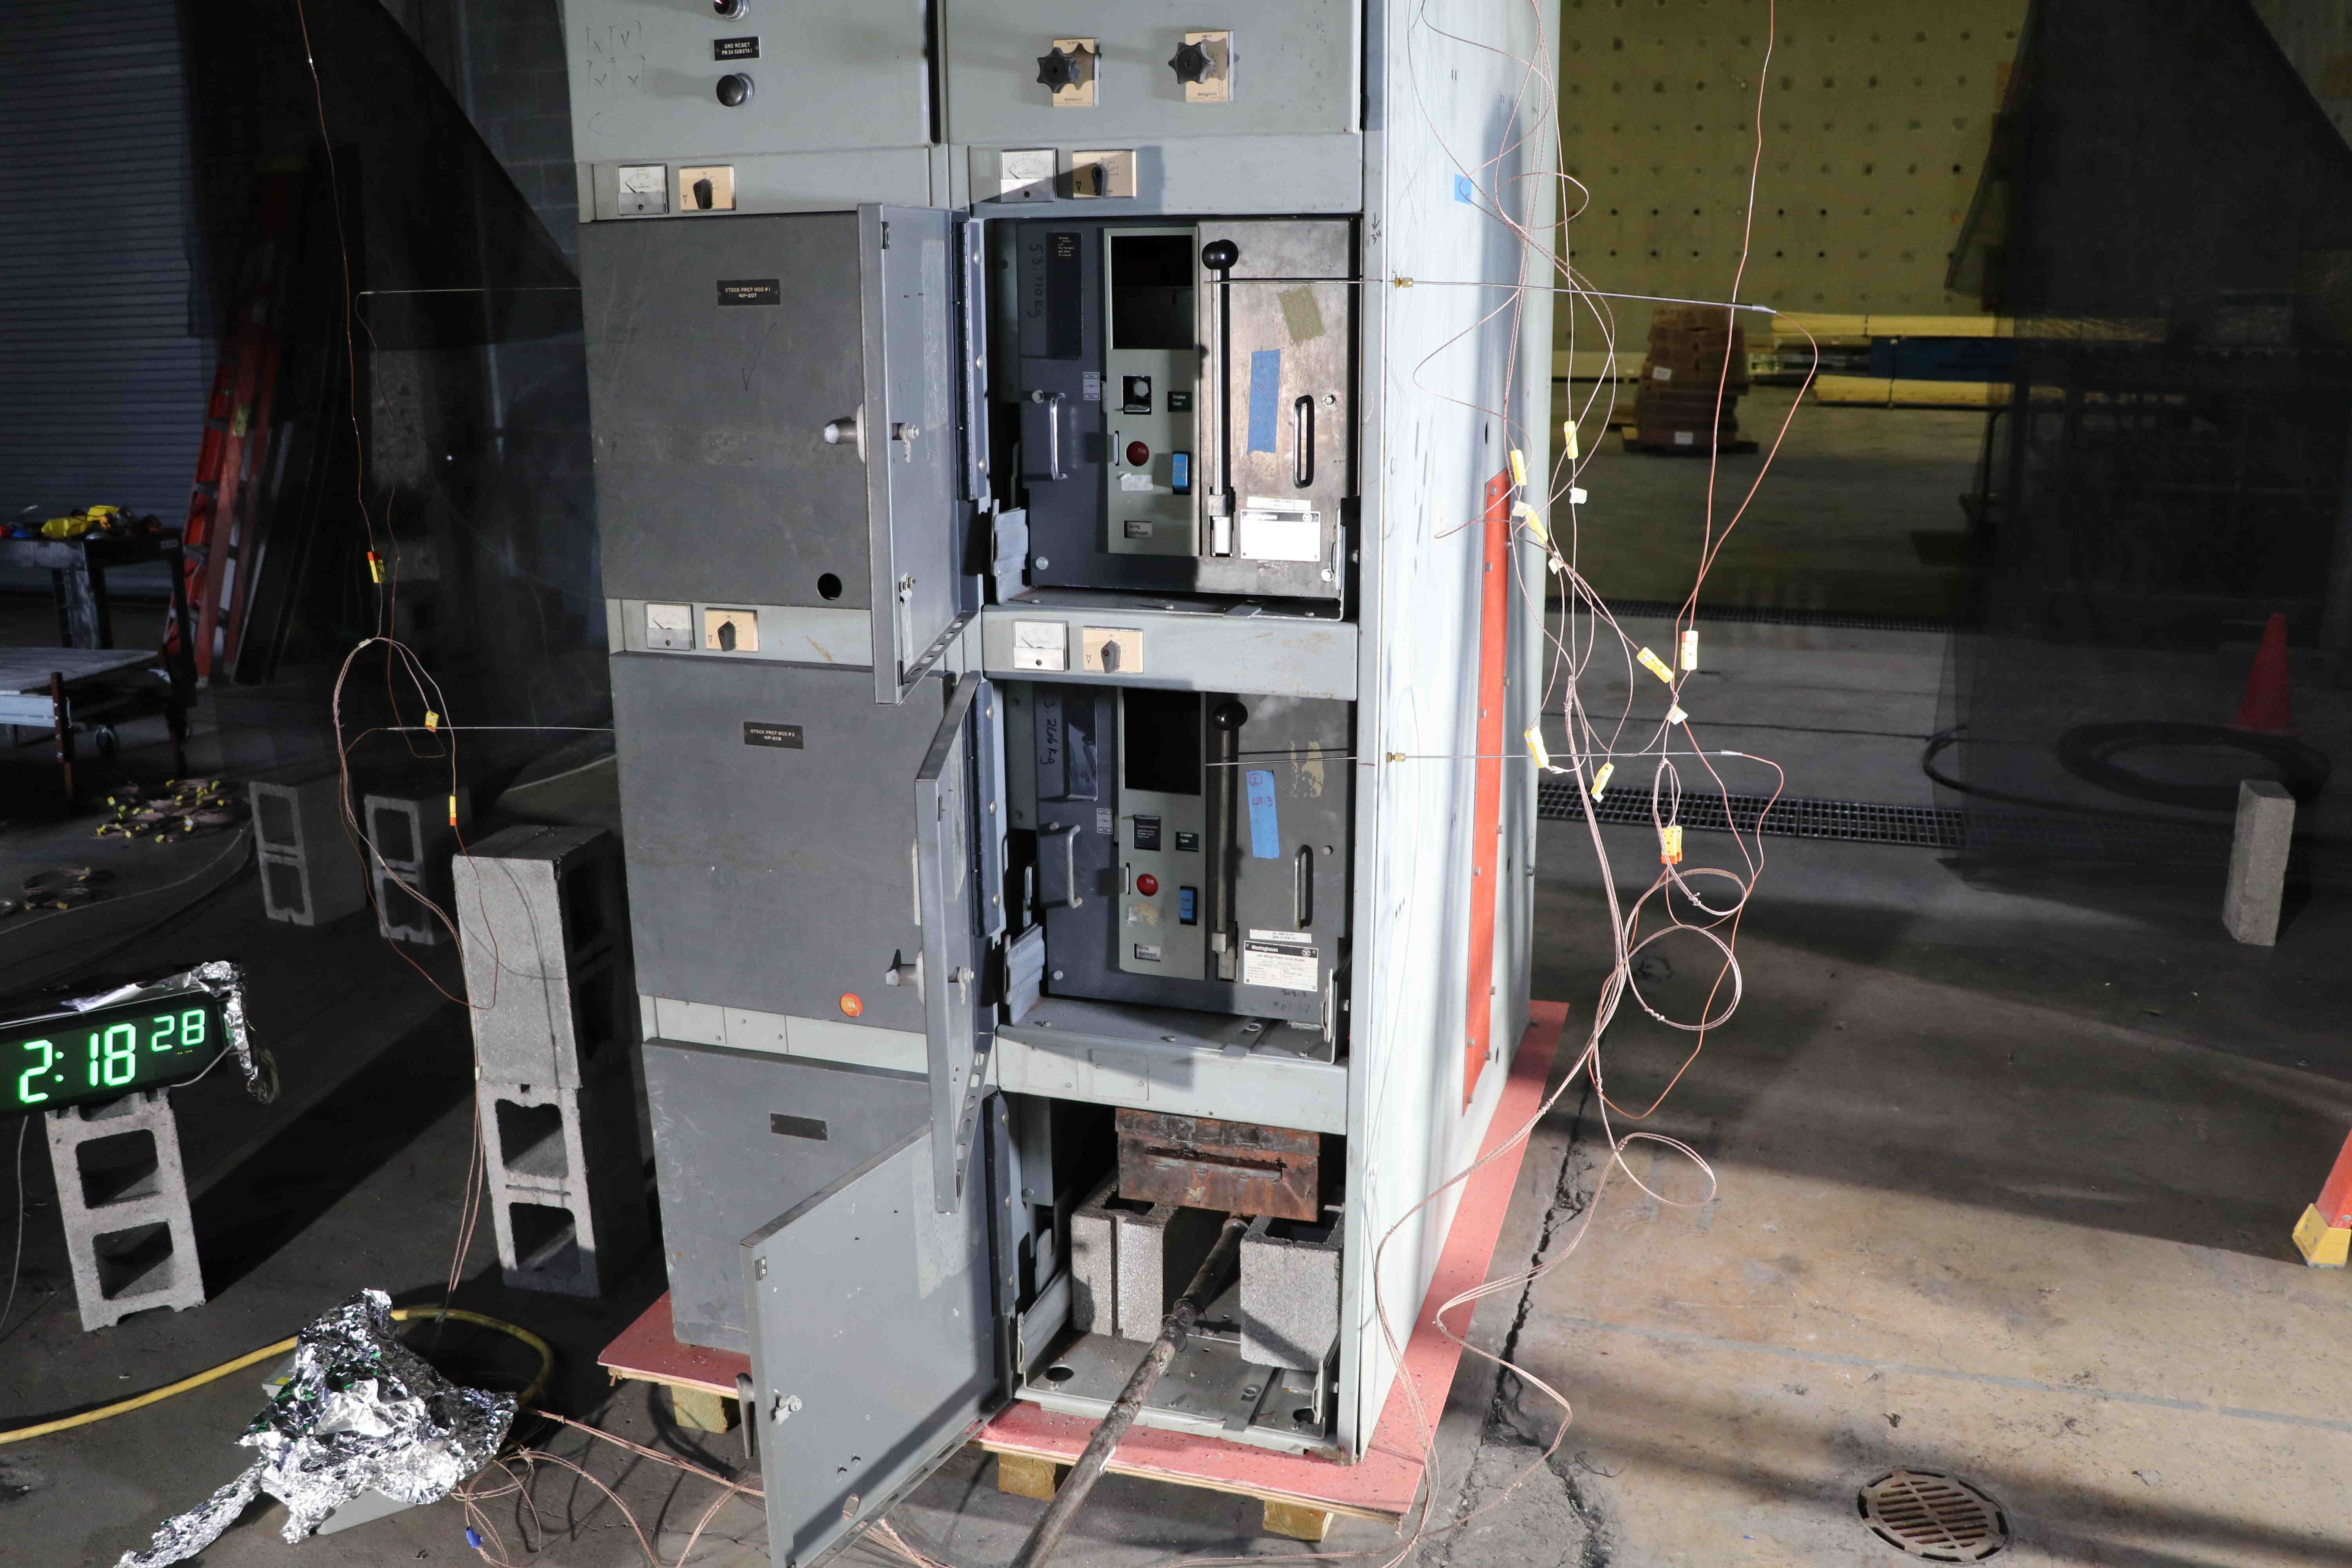
\includegraphics[width=6.5in]{../FIGURES/Westinghouse}
\caption[Photograph of Westinghouse enclosure] {Photograph of the Westinghouse enclosure. A gas burner has replaced the lowest level breaker.}
\label{fig:Cabinet_2}
\end{figure}

\subsection{Description of Experiments}

In each experiment, a low voltage circuit breaker with nominal dimensions of 30~cm by 40~cm by 30~cm and mass 47~kg was the primary combustible whose non-metallic mass consists of polymeric insulating materials such as glass-polyester and thermoset composite resins. Additionally, plastic wire harnesses, SIS wire\footnote{SIS Wire identifies a range of single-core wires for use in electrical switchboards and panels.}, and circuit boards were found mainly in the compartment above the breaker, as seen in Fig.~\ref{fig:Contents}. There were only a few jacketed, multi-conductor cables. The compartment below the breaker was largely empty of combustibles. No attempt was made to remove and weigh the combustible material because doing so would have potentially changed its burning behavior; however, representative samples (~approxmately 5~g to 10~g of each material) of ten of the most commmon electrical components in the compartment (e.g., wiring, switches, circuit boards, and electrical insulation materials) were removed prior to the experiments for microscale combustion calorimetry (MCC) measurements of their heat of combustion. Estimates of total combustible mass in the compartment were then be made by dividing the integral of the heat release rate with time (kJ) by this measured heat of combustion (kJ/kg). These results are presented in Sec.~\ref{sec:results}.

\begin{figure}[ht]
\centering
\includegraphics[width=6.5in]{../FIGURES/Contents}
\caption[Photograph of instrumentation above the breaker] {Photograph of instrumentation above the breaker. A few cables have been added to replace those removed previously.}
\label{fig:Contents}
\end{figure}

The breakers were ignited using a nominal 30~cm (12~in) square natural gas burner positioned approximately 20~cm (8~in) beneath the circuit breaker, as shown in Fig.~\ref{fig:Burner}. The burner's heat release rate\footnote{The relative expanded uncertainty (95~\% confidence interval) of the heat release rate measurement under the hood used in these experiments is 4~\% for natural gas and 7~\% for ``generic combustibles''~\cite{bryant2019nist}.} was set to approximately 100~kW. After sustained ignition of the circuit breaker was observed, the burner was turned off and the enclosure fire was allowed to continue burning until the measured heat release rate decreased below 10~kW, at which point the small remaining fires were extinguished.

\begin{figure}[ht]
\centering
\includegraphics[width=6.5in]{../FIGURES/Burner}
\caption[Position of the burner] {Position of the burner under the breaker in Test~34.}
\label{fig:Burner}
\end{figure}

Sheathed thermocouples (K-type, sheath diameter 3~mm) were installed 15~cm (6~in) below the ceiling of each compartment to provide a measurement of the gas temperature within. Thermocouples were also embedded within representative items (``slugs'') that were placed directly above each circuit breaker: 7-conductor thermoplastic electrical cable segments and 6061~aluminum alloy rods, both approximately  15~cm (6~in) in length and 13~mm in diameter. The heat capacity of these objects can be expressed in terms of the product of their density, specific heat, and cross sectional area, $\rho c A$, in units of kJ/K/m; that is, the amount of energy required to raise a 1~m segment 1~K. The heat capacity of the aluminum rod is approximately 0.31~kJ/K/m and the cable segment is approximately 0.36~kJ/K/m. Figure~\ref{oven} displays the measured temperature of each when placed in a convection oven whose temperature was raised to 300~$^\circ$C.

\begin{figure}[!ht]
\centering
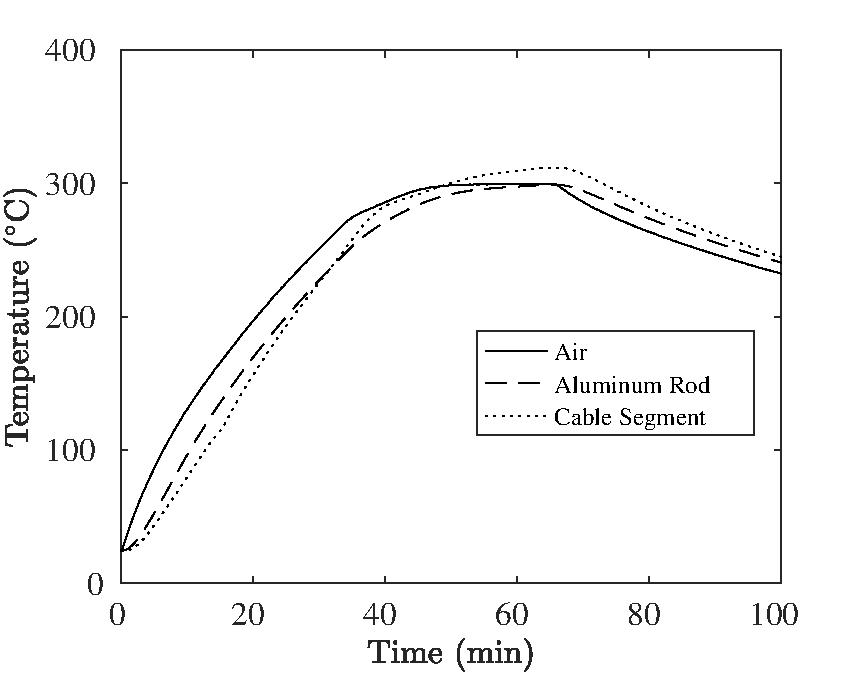
\includegraphics[height=3.0in]{../SCRIPT_FIGURES/Oven_Test}
\caption[Measured temperatures of slug calorimeters in a convection oven]{Measured temperatures of a 1/2 inch aluminum rod and cable segment in a convection oven.}
\label{oven}
\end{figure}

Photographs of the enclosures used in this work are shown in Figs.~\ref{fig:Cabinet_1} and \ref{fig:Cabinet_2}. Each enclosure is approximately 2.2~m (87~in) tall, 0.4~m (16~in) wide, and 1.0~m (40~in) deep. Some of the enclosures have ventilation panels near the top and bottom, and all have seams and small openings to accommodate wiring, bus bars, door panels, and so on. No attempt was made to seal these various gaps and openings except in Experiment~34 where a burned out instrument panel was covered by a steel plate, and in Experiment~35, where a hole in the top of the enclosure was covered by a steel plate.



\subsection{Experimental Results}
\label{sec:results}


The measurements of the heat release rate of the breakers were conducted in October of 2023 and January of 2024. Nominal results are listed in Table~\ref{matrix} and details can be found on the following pages. For each experiment, the nominally 100~kW natural gas burner was sustained until it appeared that the breaker had begun to burn. For the first two experiments, the burner was sustained longer than necessary, as evidenced by Exp.~35 where the breaker was able to sustain a fire after four minutes of exposure from the burner.

Overall, the breakers within the ABB enclosures did sustain a fire beyond the time when the burner was extinguished. However, the Westinghouse breakers did not appear to burn without the aid of the gas burner, even though the non-metallic materials within the breaker clearly showed evidence after the experiment of having pyrolized.

The ``Peak HRR'' in Table~\ref{matrix} indicates the maximum value of the heat release rate of the enclosure contents; that is the total heat release rate minus that of the natural gas burner. The ``Total HR'' (Total Heat Release) is the total energy released less the burner's energy; that is, the energy of the contents alone. The ``Mass Consumed'' is the Total HR divided by an estimated\footnote{The uncertainty of the estimated heat of combustion is difficult to quantify. The estimated value of 25~MJ/kg is merely the center point of the interval between 20~MJ/kg and 30~MJ/kg which is a typical range for the  various plastics found within the enclosure.} heat of combustion of 25~MJ/kg for the combustible materials within the enclosure. The peak ``slug'' and gas temperatures are comparable and represent uniform conditions within the burning breaker and instrument compartments.


\begin{table}[ht]
\begin{center}
\caption[Summary of Experimental Results]{Summary of Experimental Results. The values of temperature are rounded to the nearest 10~$^\circ$C which is much greater than the uncertainty of the thermocouples used in the experiments. The listed times are rounded to the nearest minute.}
\label{matrix}
\begin{tabular}{|c|c|c|c|c|c|c|c|c|}
\hline
Exp.   &                & Peak           & Total      & Mass            & Time            & Burner       & Peak Slug    & Peak Gas      \\
No.    & Make           & HRR            & HR         & Consumed        & to Peak         & Duration     & Temp.        & Temp.         \\
       &                & [kW]           & [MJ]       & [kg]            & [min]           & [min]        & [$^\circ$C]  & [$^\circ$C]   \\ \hline
33     & ABB            & 250$\pm$18     & 387$\pm$27 & 15.5$\pm$3.3    & 11              & 10           & 770          & 860           \\ \hline
34     & ABB            & 140$\pm$10     & 192$\pm$13 & 7.7$\pm$1.6     & 9               & 8            & 680          & 700           \\ \hline
35     & ABB            & 200$\pm$14     & 230$\pm$16 & 9.2$\pm$1.9     & 20              & 4            & 680          & 670           \\ \hline
40     & West.          & 30$\pm$14      & 60$\pm$4   & 2.4$\pm$0.5     & 28              & 60           & 160          & 650           \\ \hline
41     & West.          & 100$\pm$7      & 280$\pm$20 & 11.2$\pm$2.2    & 40              & 60           & 150          & 700           \\ \hline
\end{tabular}
\end{center}
\end{table}

The breaker that was burned in Exp.~35 was weighed before and after the experiment. Its original mass was 47.8~kg and its final mass was 44.1~kg. The uncertainty of the load cell is approximately 1~g, which is far exceeded by the uncertainty due to extracting the burned breaker from the enclosure and separating out materials that were or were not part of the original breaker. Thus, the estimated combustible mass of the breaker is taken as 3.7~kg~$\pm$~0.1~kg.

Using the measured mass loss of the breaker and the estimates of the mass consumed in the three experiments, it is possible to estimate the distribution of combustible mass in the lower, middle, and upper compartments of the enclosure. In Exp.~33, the fire consumed the contents of a lower, middle and three upper compartments. In Exp.~34, the fire consumed a lower and middle compartment. In Exp.~35, the fire consumed a lower, middle, and upper compartment. Taking the combustible load of the middle compartment to be 3.7~kg, the estimated mass loss of the breaker, a least squares regression yields an estimate of 3.5~kg for the lower compartment and 2.7~kg for the upper. The 3.5~kg estimate for the lower compartment can be taken as all of the combustibles in the lower and middle compartment minus the breaker itself. These estimated combustible loads fall well within the uncertainty bounds for the total mass consumption listed in Table~\ref{matrix}.

The heat release rate of a fire contained within a single compartment is limited by the air supplied through openings in the back and side of the enclosure and the opening in the front door of the compartment that is created when the instrument panel melts/burns away. For the enclosures tested, this opening is approximately 15~cm (6~in) wide by 30~cm (12~in) tall. A useful correlation~\cite{SFPE:Walton} used in compartment fire modeling states that air is entrained into a flashed over compartment at a rate given by
\begin{equation}
   \dot{m}_{\rm a} = 0.5  \, A \, \sqrt{H}  \approx 0.0123 \; \hbox{kg/s}
\end{equation}
where $H$ is the opening height (0.3~m) and $A$ is the opening area (0.045~m$^2$). With this estimate, the heat release rate can be estimated
\begin{equation}
   \dot{Q} = Y_{\rm O_2,\infty} \, E \, \dot{m}_{\rm a} \approx 37 \; \hbox{kW}
\end{equation}
where $Y_{\rm O_2,\infty}\approx 0.23$ is the oxygen mass fraction of air and $E\approx 13\,100$~kJ/kg is the approximate amount of energy released per unit mass of oxygen consumed.

Evidence for the estimated heat release rate associated with the opening of the instrument panel can be seen in Exp.~35 where the upper compartment opens up at approximately 19~min, at which time the HRR increases rapidly by approximately 40~kW. The increased ventilation through the front door adds to the existing ventilation through the back of the enclosure. Collectively, these openings supply the air needed to support an HRR of approximately 100~kW per compartment.


\subsubsection{Material Property Measurements}

Material samples were taken from the various circuit breakers to better understand their burning behavior using a Microscale Combustion Calorimeter\footnote{Deatak MCC-3 equipped with a paramagnetic oxygen sensor and calibrated according to ASTM~D7309~\cite{ASTM_D7309}} (MCC), an apparatus in which a specimen of known mass is thermally decomposed in nitrogen at a constant heating rate and then burned in oxygen to determine its heat of combustion.

MCC experiments were conducted in December, 2023. The material samples were subjected to a 80~mL/min nitrogen stream starting at a temperature of 75~°C, increasing linearly to 750~°C at a heating rate of 60~K/min. The pyrolyzed gases were combusted in an oxygen stream of 20~mL/min. Tests were repeated at least three times for each material. Nominal results are listed in Table~\ref{MCC}. The average heat of combustion of the materials tested is approximately \#**. Also reported in this table are the onset temperature and Fire Growth Capacity, FGC. The FGC is a physically based parameter for early stage fire growth, derived from a simple burning model, that has been shown to rank commercial materials according to their behavior in bench scale flame and fire tests. The onset temperature  is calculated as...[**Isaac will complete this section and add the corresponding reference]. Details of these calculations are provided elsewhere~\cite{DOT/FAA/TC-20/30}.

\begin{table}
\begin{center}
\caption[MCC Measurements]{MCC Measurements. Uncertainty in reported heat of combustion represents an expanded uncertainty ($U_c$; 95~\% confidence interval, coverage factor = 2).  The primary sources of uncertainty in this measurement include (1) Uncertainty in measured solid residue yield, **3\%; (2) uncertainty of oxygen consumption calorimetry measurements~\cite{Huggett:1}; and test repeatability, calculated as **1 standard deviation of the mean.}
\label{MCC}
\begin{tabular}{ccccc}
\hline
Matl.  & Heat of        & Solid Residue    & Onset              & Fire Growth                   \\
No.    & Combustion     & Yield            & Temperature        & Capacity (FGC)          \\
       & (kJ/g)         & (g/g)            & (°C)               & (J/(g~K))    \\
\hline
1      &  ?? $\pm$ ??   & 0.xx $\pm$ ??    &                    &              \\
2      &  ?? $\pm$ ??   & 0.xx $\pm$ ??    &                    &              \\
3      &  13.9 $\pm$ ?? & 0.29 $\pm$ ??    &                    &              \\
4      &  30.8 $\pm$ ?? & 0.02 $\pm$ ??    &                    &              \\
5      &  25.7 $\pm$ ?? & 0.00 $\pm$ ??    &                    &              \\
6      &  28.3 $\pm$ ?? & 0.10 $\pm$ 0.00  &                    &              \\
7      &  21.9 $\pm$ ?? & 0.40 $\pm$ ??    &                    &              \\
8      &  9.6 $\pm$ ??  & 0.02 $\pm$ ??    &                    &              \\
9      &  29.7 $\pm$ ?? & 0.24 $\pm$ ??    &                    &              \\
10     &  14.8 $\pm$ ?? & 0.57 $\pm$ ??    &                    &              \\
\hline
\end{tabular}
\end{center}
\end{table}


\clearpage

\subsubsection{Experiment 33}

Referring to the photographs shown in Fig.~\ref{fig:Test_33_photos}, the natural gas burner was positioned near the top of the lower left compartment of the enclosure, approximately 20~cm (8~in) below the breaker that is located in the center-left compartment. The fire ignited the breaker after approximately 2~min and then spread to the compartment above. As evidenced by the compartment temperatures shown in the upper right plot of Fig.~\ref{fig:Test_33}, the fire then spread to the two adjacent compartments along the top of the enclosure. The gas temperatures shown in Fig.~\ref{fig:Test_33} indicate that the fire spread from one compartment to the next in approximately 10~min. The compartments are separated by two steel walls.

\begin{figure}[!h]
\begin{tabular*}{\textwidth}{l@{\extracolsep{\fill}}r}
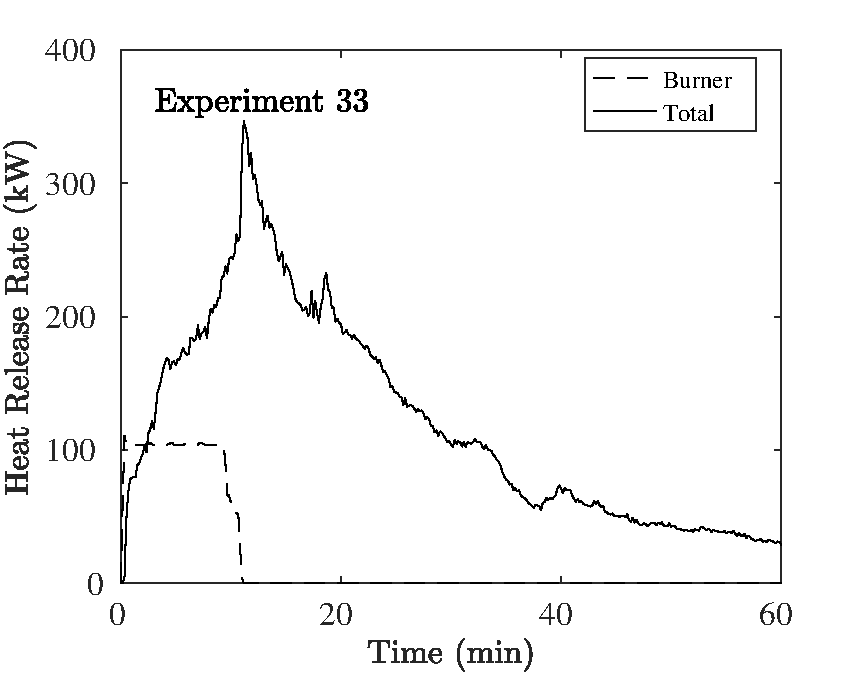
\includegraphics[height=2.65in]{../SCRIPT_FIGURES/Test_33_HRR} &
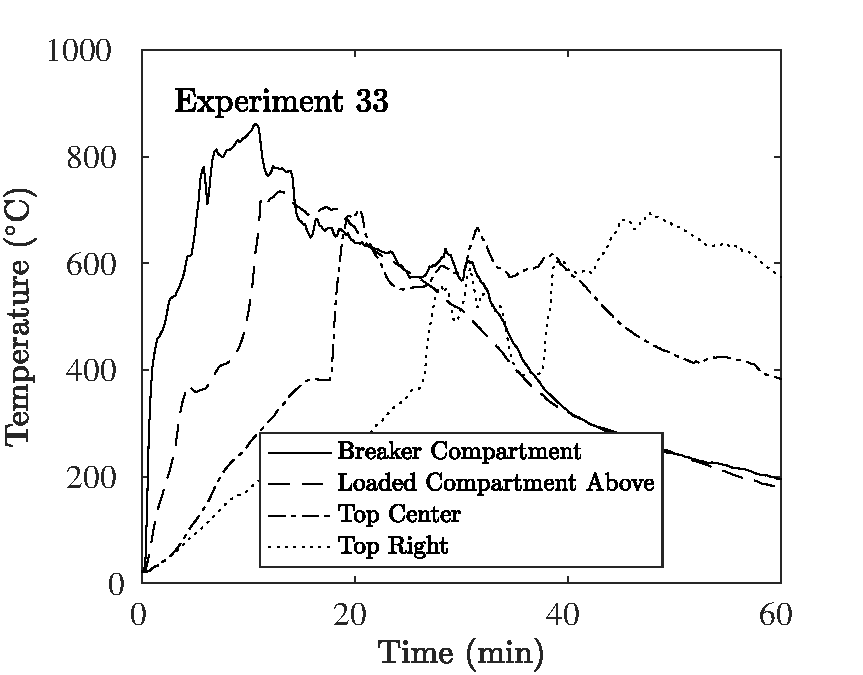
\includegraphics[height=2.65in]{../SCRIPT_FIGURES/Test_33_Gas_TC} \\
\multicolumn{2}{c}{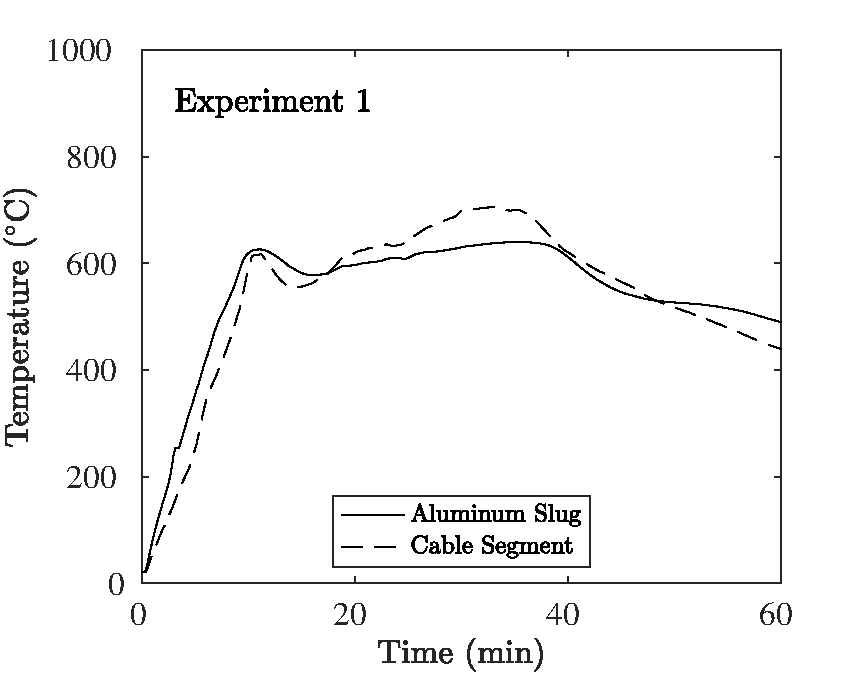
\includegraphics[height=2.65in]{../SCRIPT_FIGURES/Test_33_Slug_TC}}
\end{tabular*}
\caption[HRR and temperatures of Exp.~33]{Heat release rate (upper left), gas temperatures (upper right), and slug temperatures for Exp.~33.}
\label{fig:Test_33}
\end{figure}

\begin{figure}[p]
\centering
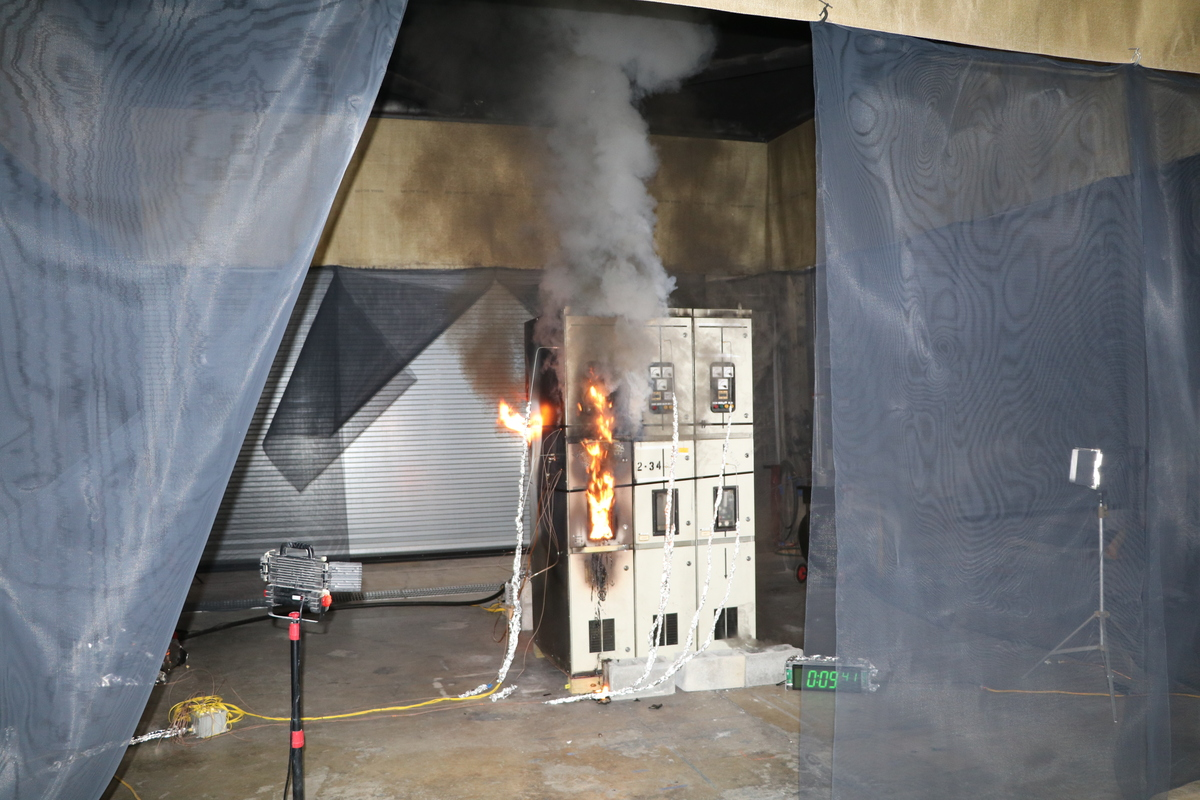
\includegraphics[height=2.75in]{../FIGURES/Test_33_9_min} \\
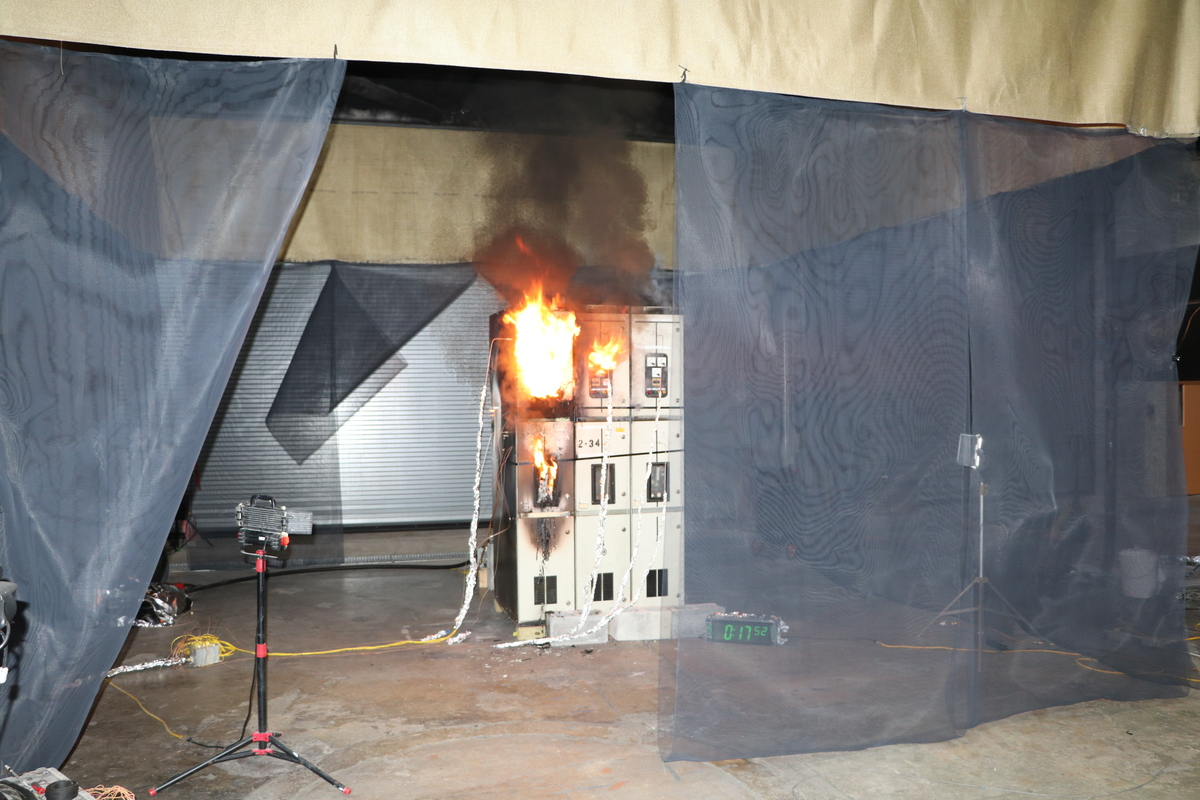
\includegraphics[height=2.75in]{../FIGURES/Test_33_17_min} \\
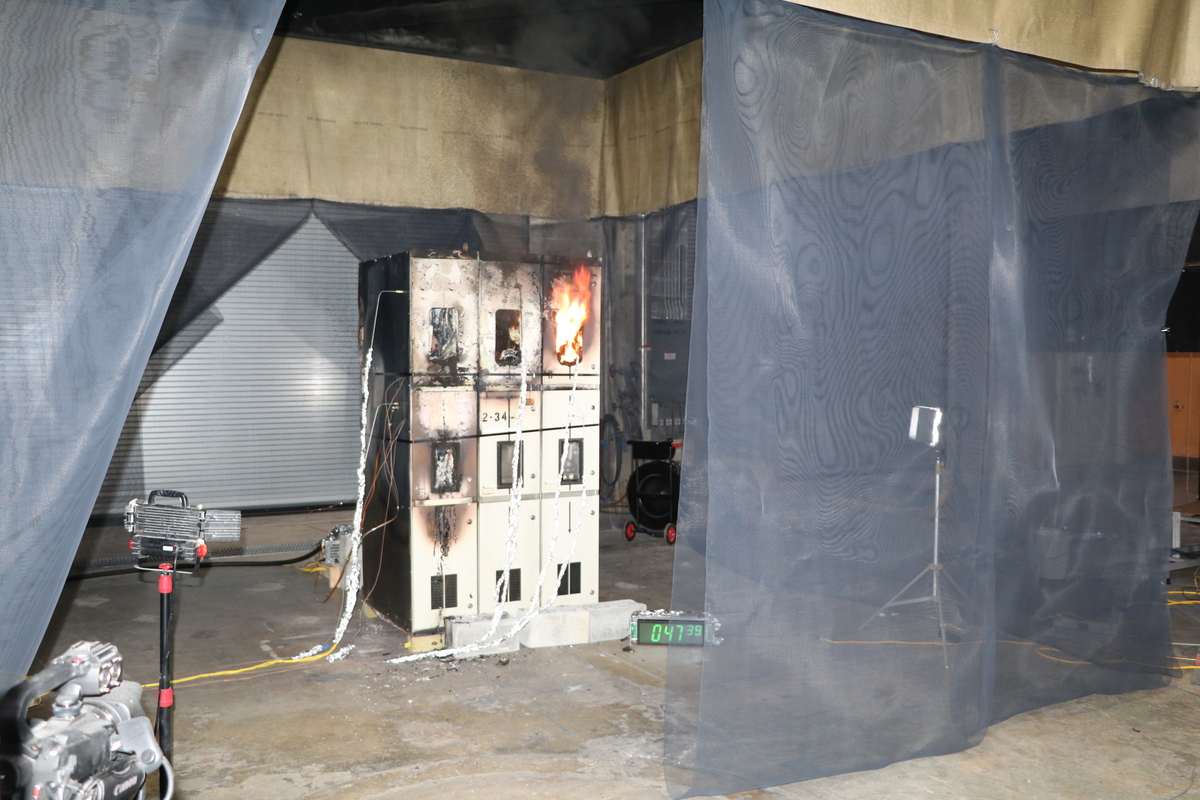
\includegraphics[height=2.75in]{../FIGURES/Test_33_47_min}
\caption[Photographs of Experiment~33]{Photographs of Experiment~33, 9~min, 17~min, and 47~min after ignition of the burner which was located in the lower left compartment.}
\label{fig:Test_33_photos}
\end{figure}



\clearpage

\subsubsection{Experiment 34}

The fire in Exp.~33 consumed all of the combustibles in the upper compartments of the large enclosure. However, the breakers in the center and right columns remained intact. For Exp.~34, the burner was placed beneath the breaker on the right side of the enclosure (see Fig.~\ref{fig:Test_34_photos}) with the aim of measuring its heat release rate with no combustibles in the compartment above. The gas temperature in the compartment above reaches only approximately 400~$^\circ$C because there is no significant fire in this compartment, only the heat from below.

\begin{figure}[!h]
\begin{tabular*}{\textwidth}{l@{\extracolsep{\fill}}r}
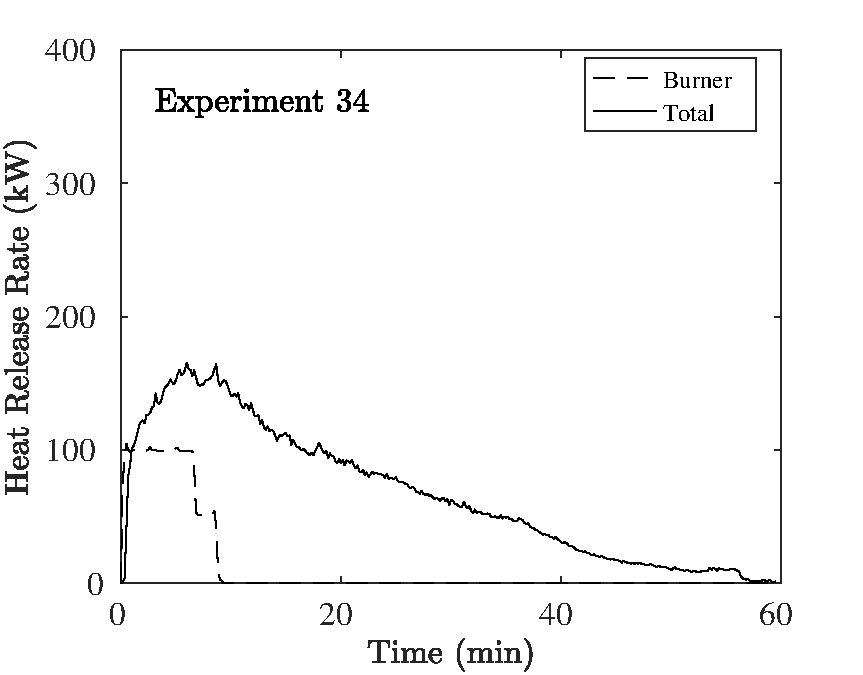
\includegraphics[height=2.65in]{../SCRIPT_FIGURES/Test_34_HRR} &
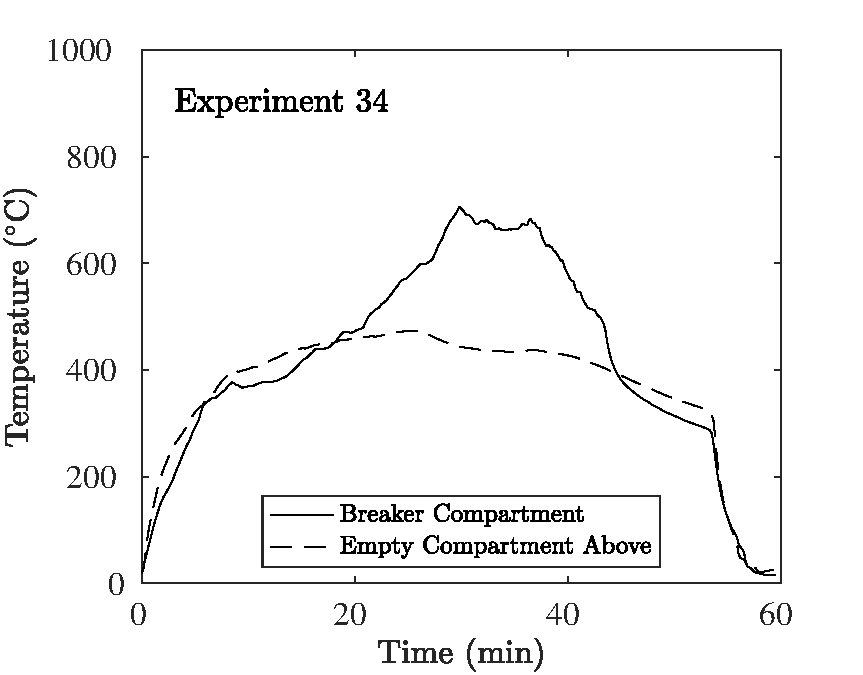
\includegraphics[height=2.65in]{../SCRIPT_FIGURES/Test_34_Gas_TC} \\
\multicolumn{2}{c}{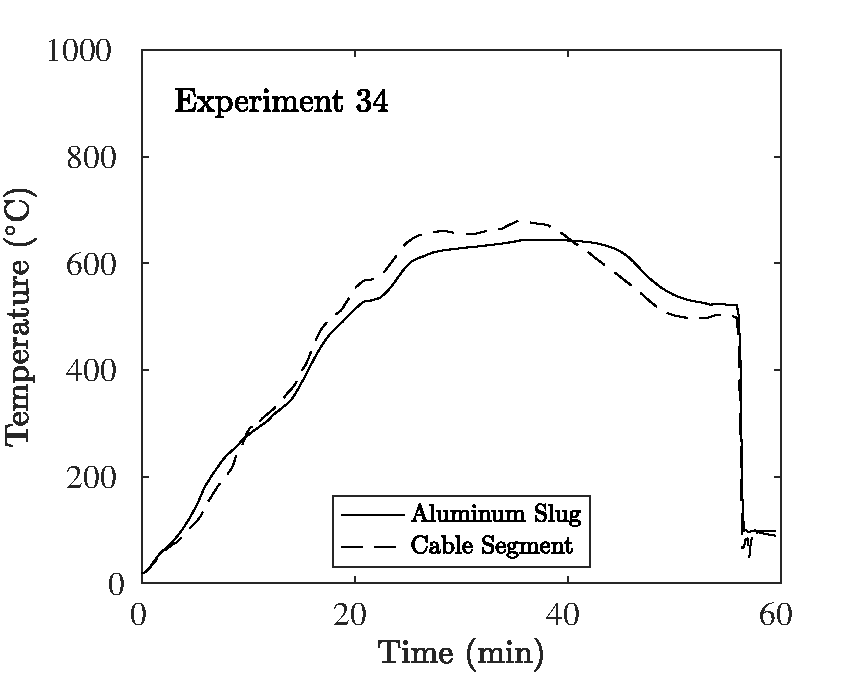
\includegraphics[height=2.65in]{../SCRIPT_FIGURES/Test_34_Slug_TC}}
\end{tabular*}
\caption[HRR and temperatures of Exp.~34]{Heat release rate (upper left), gas temperatures (upper right), and slug temperatures for Exp.~34.}
\label{fig:Test_34}
\end{figure}

\begin{figure}[p]
\centering
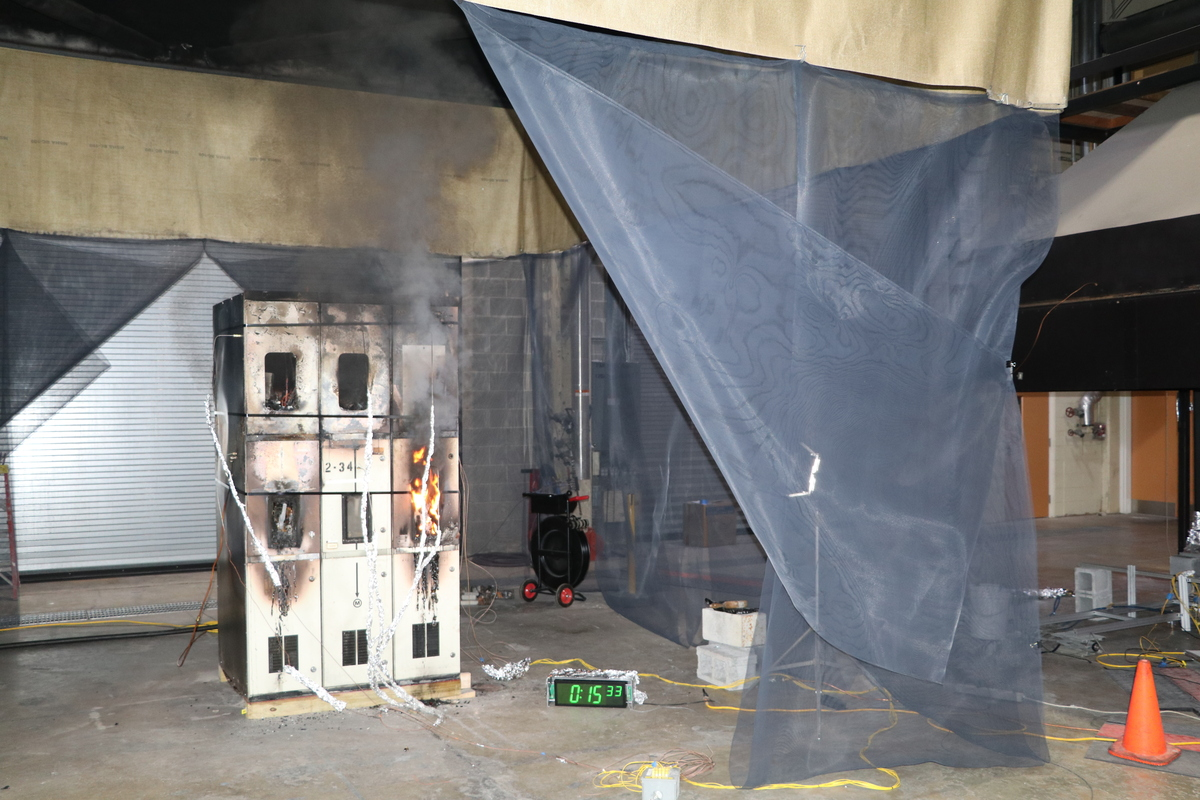
\includegraphics[height=2.75in]{../FIGURES/Test_34_15_min} \\
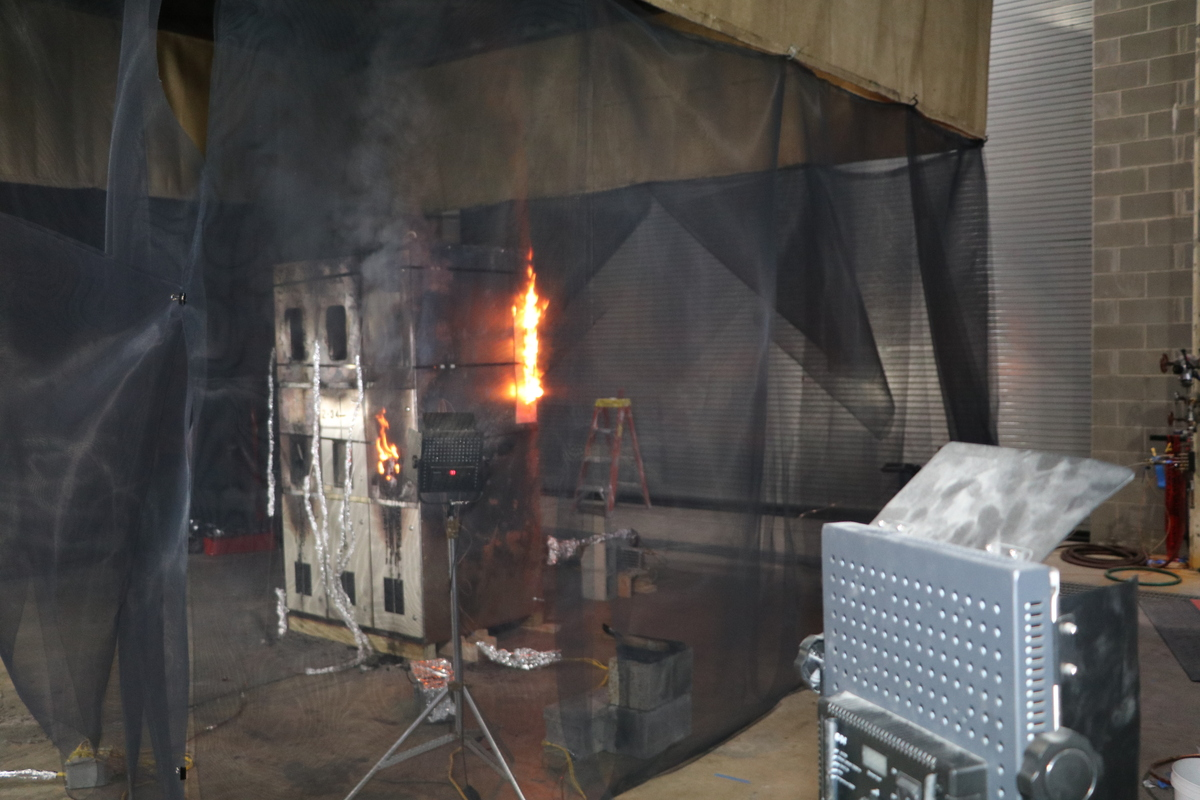
\includegraphics[height=2.75in]{../FIGURES/Test_34_30_min} \\
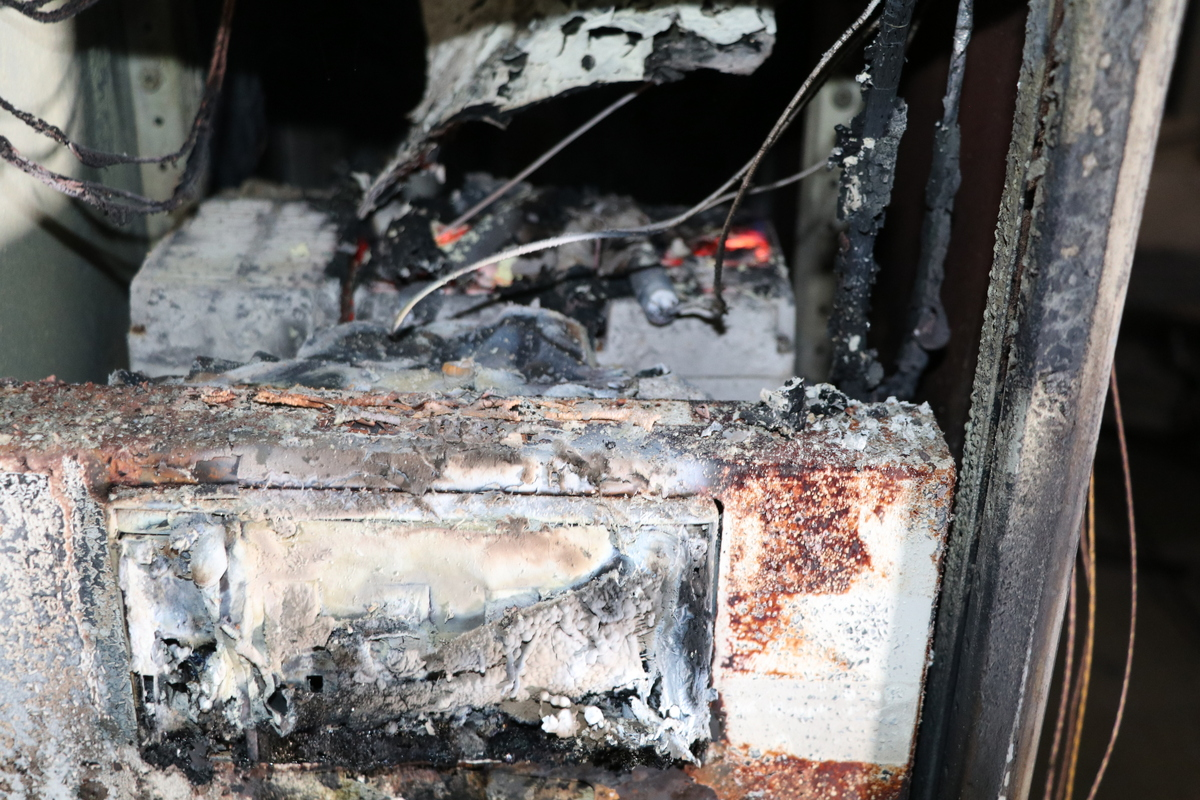
\includegraphics[height=2.75in]{../FIGURES/Test_34_60_min}
\caption[Photographs of Exp.~34]{Photographs of Exp.~34, 15~min, 30~min, and 60~min after ignition of the burner which was located in the lower right compartment. The bottom photograph shows the breaker after the experiment continues to glow red due to the heat trapped within.}
\label{fig:Test_34_photos}
\end{figure}


\clearpage

\subsubsection{Experiment 35}

Referring to Fig.~\ref{fig:Test_35_photos}, this experiment was conducted within the single-column ABB breaker enclosure, where the burner was positioned as in the previous experiments. The breaker ignited within 4~min at which time the burner was turned off. The total HRR dropped to about 50~kW at this time and then slowly increased as the fire spread from the breaker to the compartment above after approximately 18~min from the start of the experiment.

\begin{figure}[!h]
\begin{tabular*}{\textwidth}{l@{\extracolsep{\fill}}r}
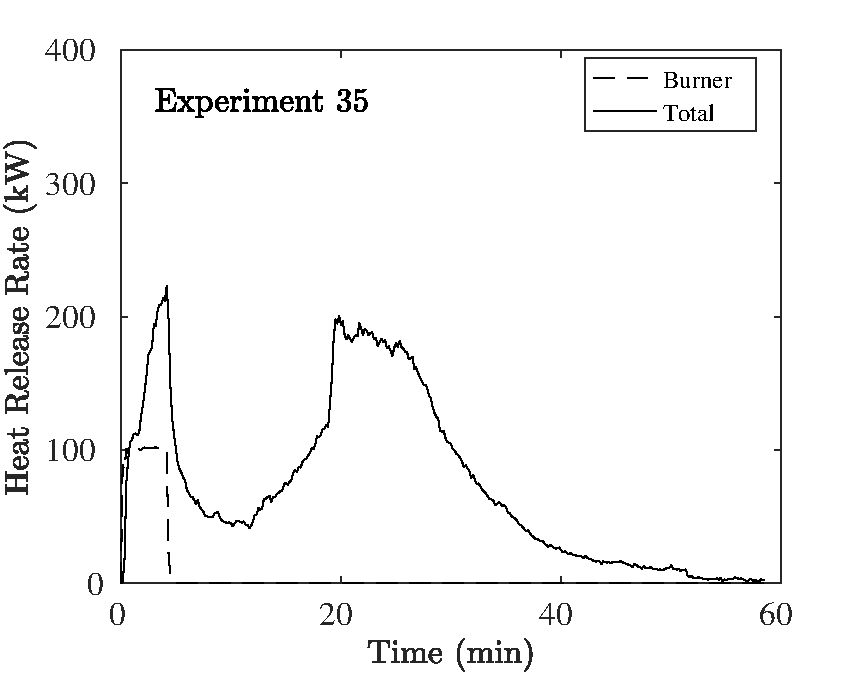
\includegraphics[height=2.65in]{../SCRIPT_FIGURES/Test_35_HRR} &
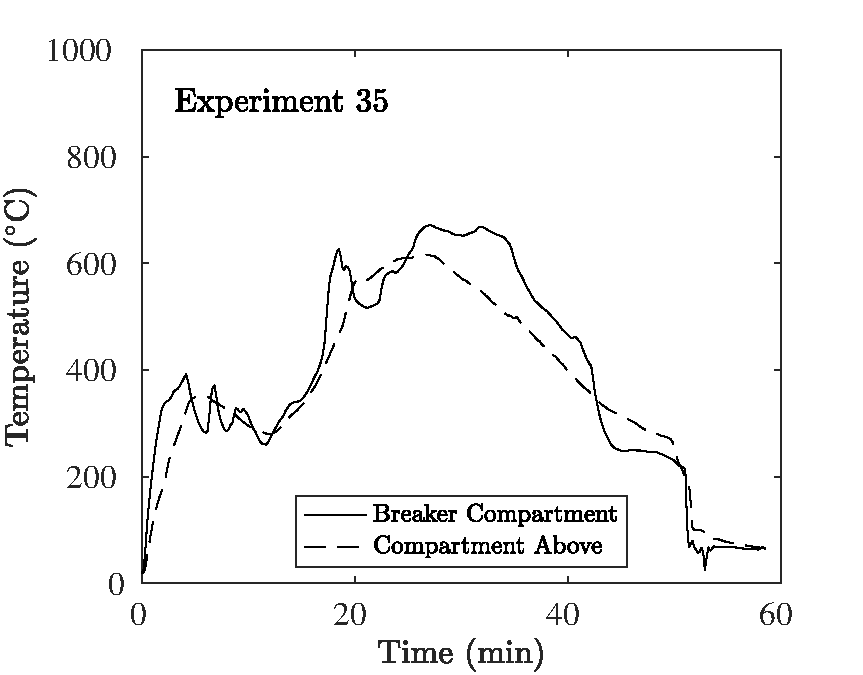
\includegraphics[height=2.65in]{../SCRIPT_FIGURES/Test_35_Gas_TC} \\
\multicolumn{2}{c}{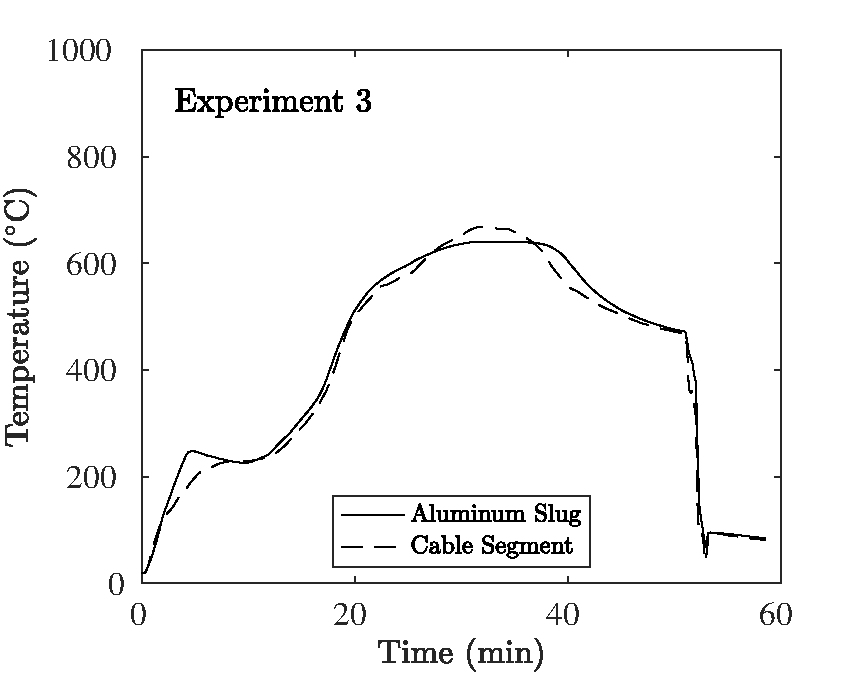
\includegraphics[height=2.65in]{../SCRIPT_FIGURES/Test_35_Slug_TC}}
\end{tabular*}
\caption[HRR and temperatures of Exp.~35]{Heat release rate (upper left), gas temperatures (upper right), and slug temperatures for Exp.~35.}
\label{fig:Test_35}
\end{figure}

\begin{figure}[p]
\centering
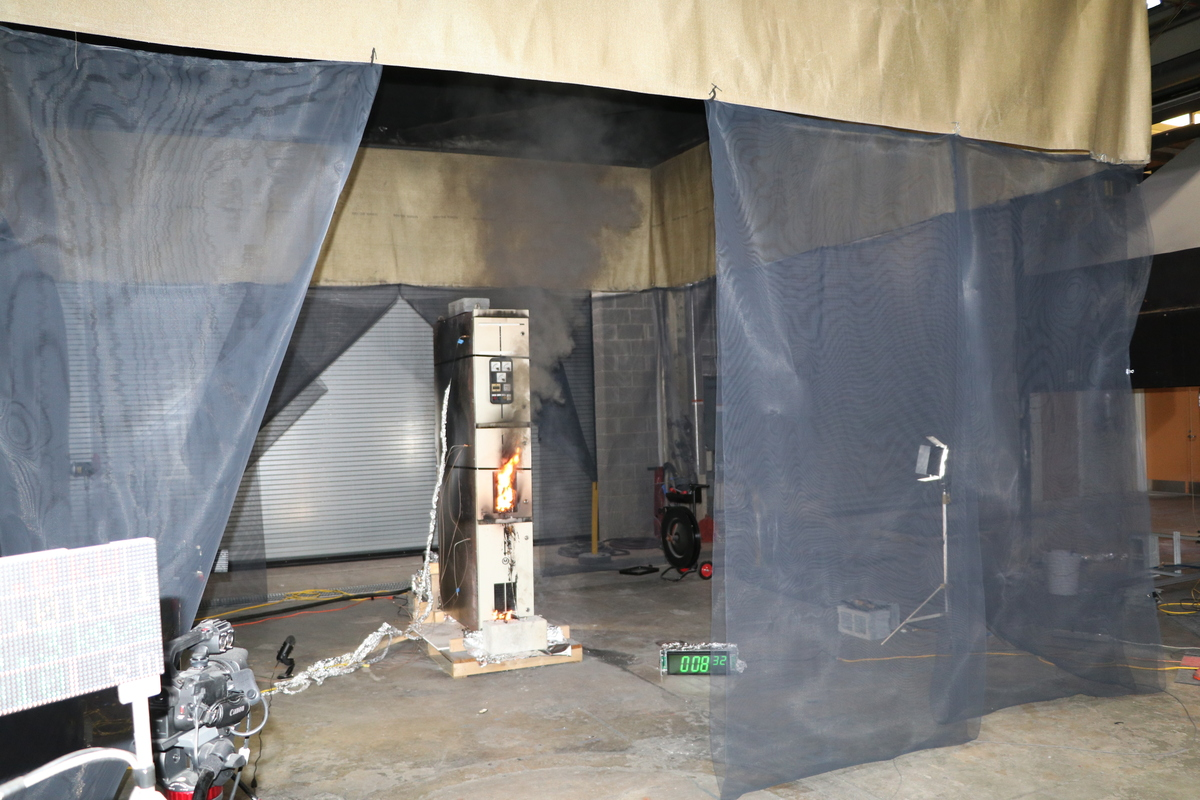
\includegraphics[height=2.75in]{../FIGURES/Test_35_8_min} \\
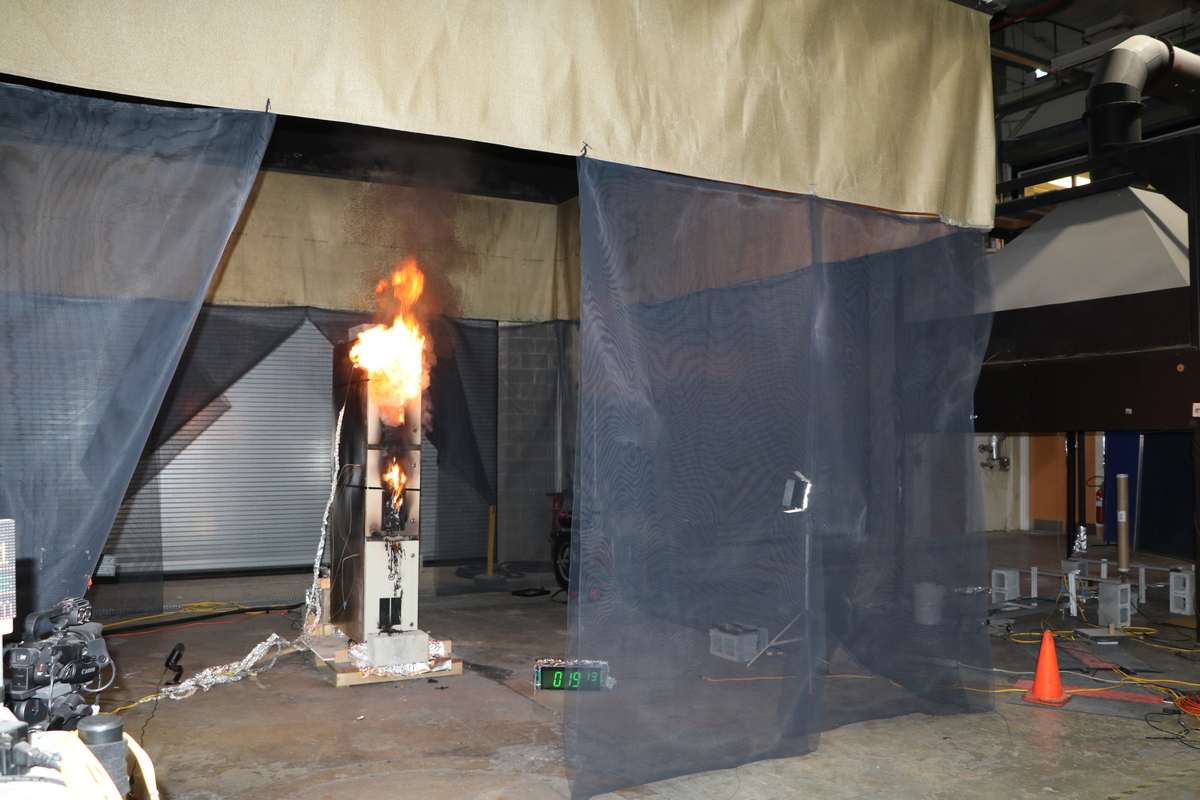
\includegraphics[height=2.75in]{../FIGURES/Test_35_19_min} \\
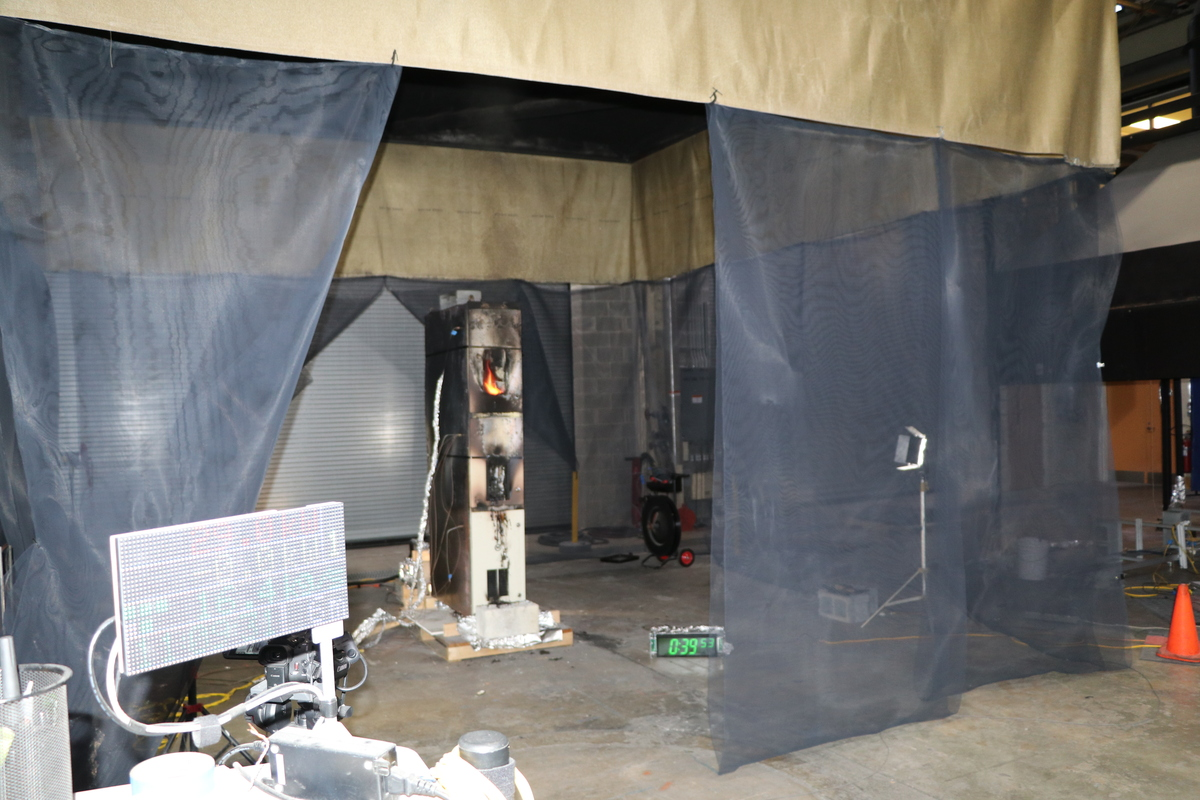
\includegraphics[height=2.75in]{../FIGURES/Test_35_39_min}
\caption[Photographs of Exp.~35]{Photographs of Exp.~35, 8~min, 19~min, and 39~min after ignition of the burner which was located in the lower compartment.}
\label{fig:Test_35_photos}
\end{figure}


\clearpage

\subsubsection{Experiment 40}

Referring to Fig.~\ref{fig:Test_40_photos}, the gas burner was positioned within the lower right compartment of a Westinghouse low voltage breaker enclosure. Breakers occupied the two compartments above, and the compartment above that was filled with approximately 0.8~kg of SIS wire. A 30~cm (12~in) wide tray containing 12 thermoplastic cables was placed approximately 30~cm (12~in) above the top of the enclosure. Thermocouples were inserted into three cables within the tray, and instrumented aluminum rods (``slugs'') were placed alongside the instrumented cables. A single sheathed thermocouple was placed at the front of each compartment. All doors on the left side of the enclosure remained closed during the experiment except the one containing the burner.

The figures below show the heat release rate of the gas burner and the total heat release rate of the burner and cables, along with the internal temperatures of the cables and slugs.

\begin{figure}[!h]
\begin{tabular*}{\textwidth}{l@{\extracolsep{\fill}}r}
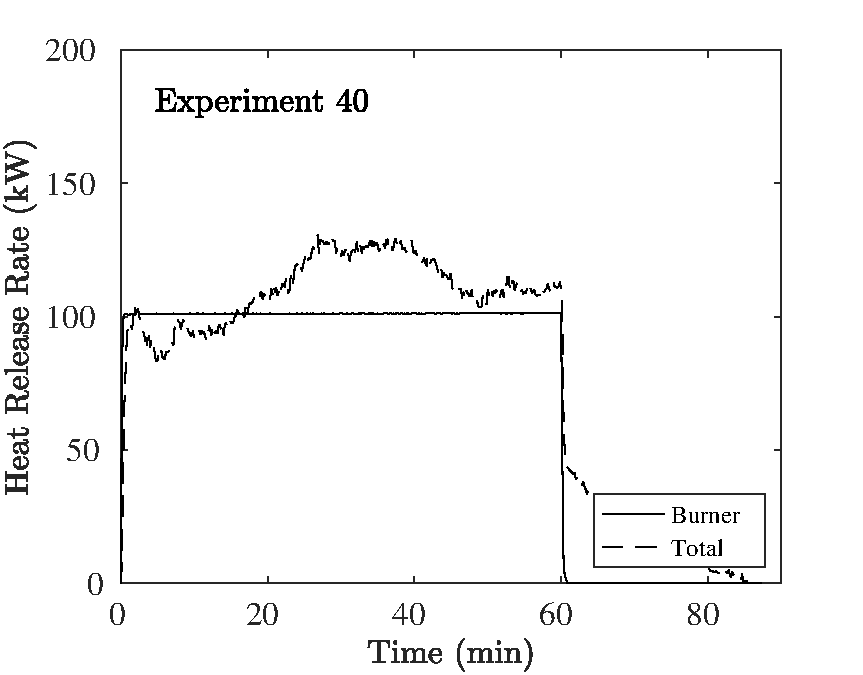
\includegraphics[height=2.65in]{../SCRIPT_FIGURES/Test_40_Plot_1} &
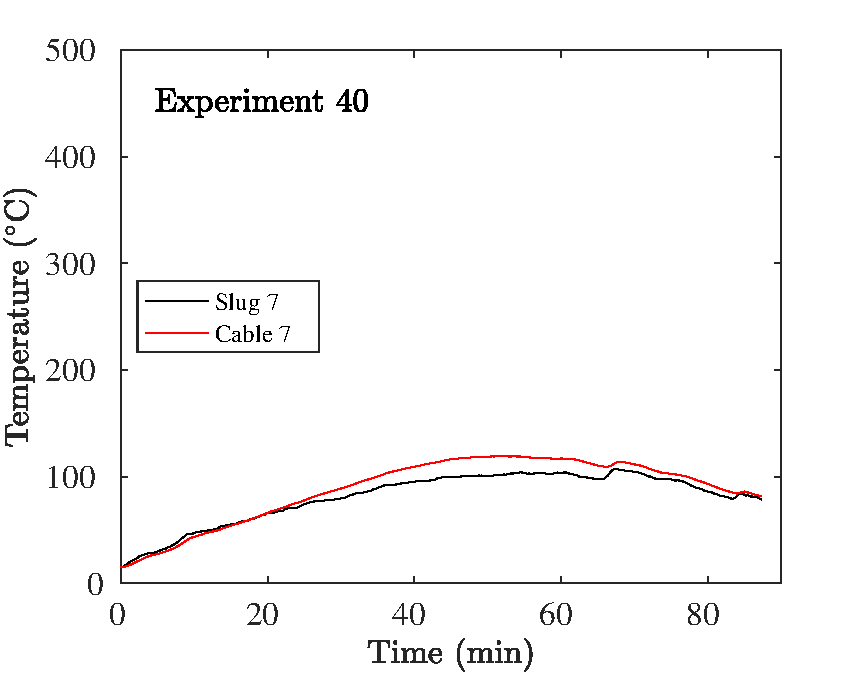
\includegraphics[height=2.65in]{../SCRIPT_FIGURES/Test_40_Plot_2} \\
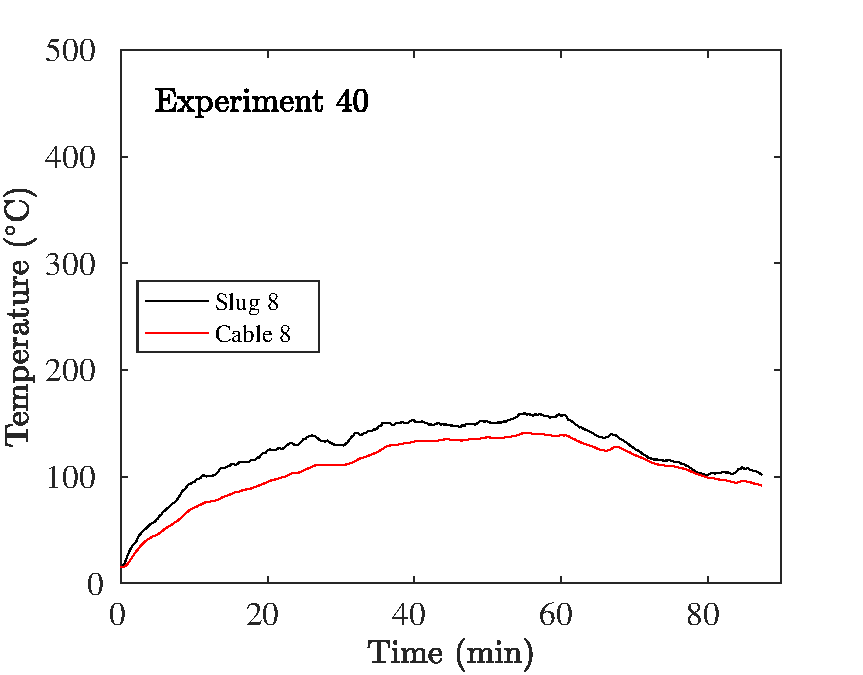
\includegraphics[height=2.65in]{../SCRIPT_FIGURES/Test_40_Plot_3} &
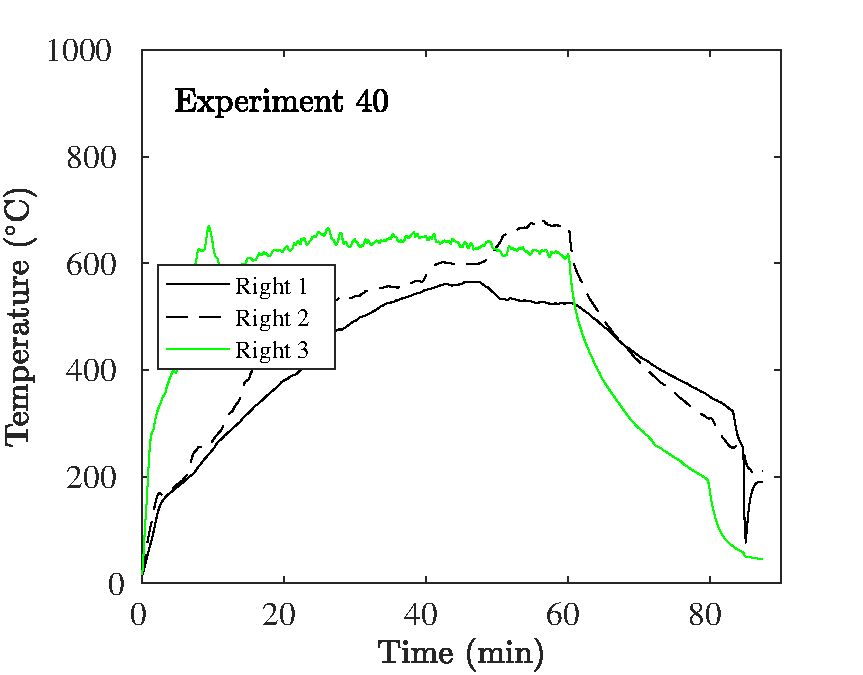
\includegraphics[height=2.65in]{../SCRIPT_FIGURES/Test_40_Plot_5}
\end{tabular*}
\caption[HRR and temperatures of Experiment 40]{Heat release rate (upper left) and various temperatures inside and above a burning breaker enclosure.}
\label{fig:Test_40}
\end{figure}

\begin{figure}[p]
\centering
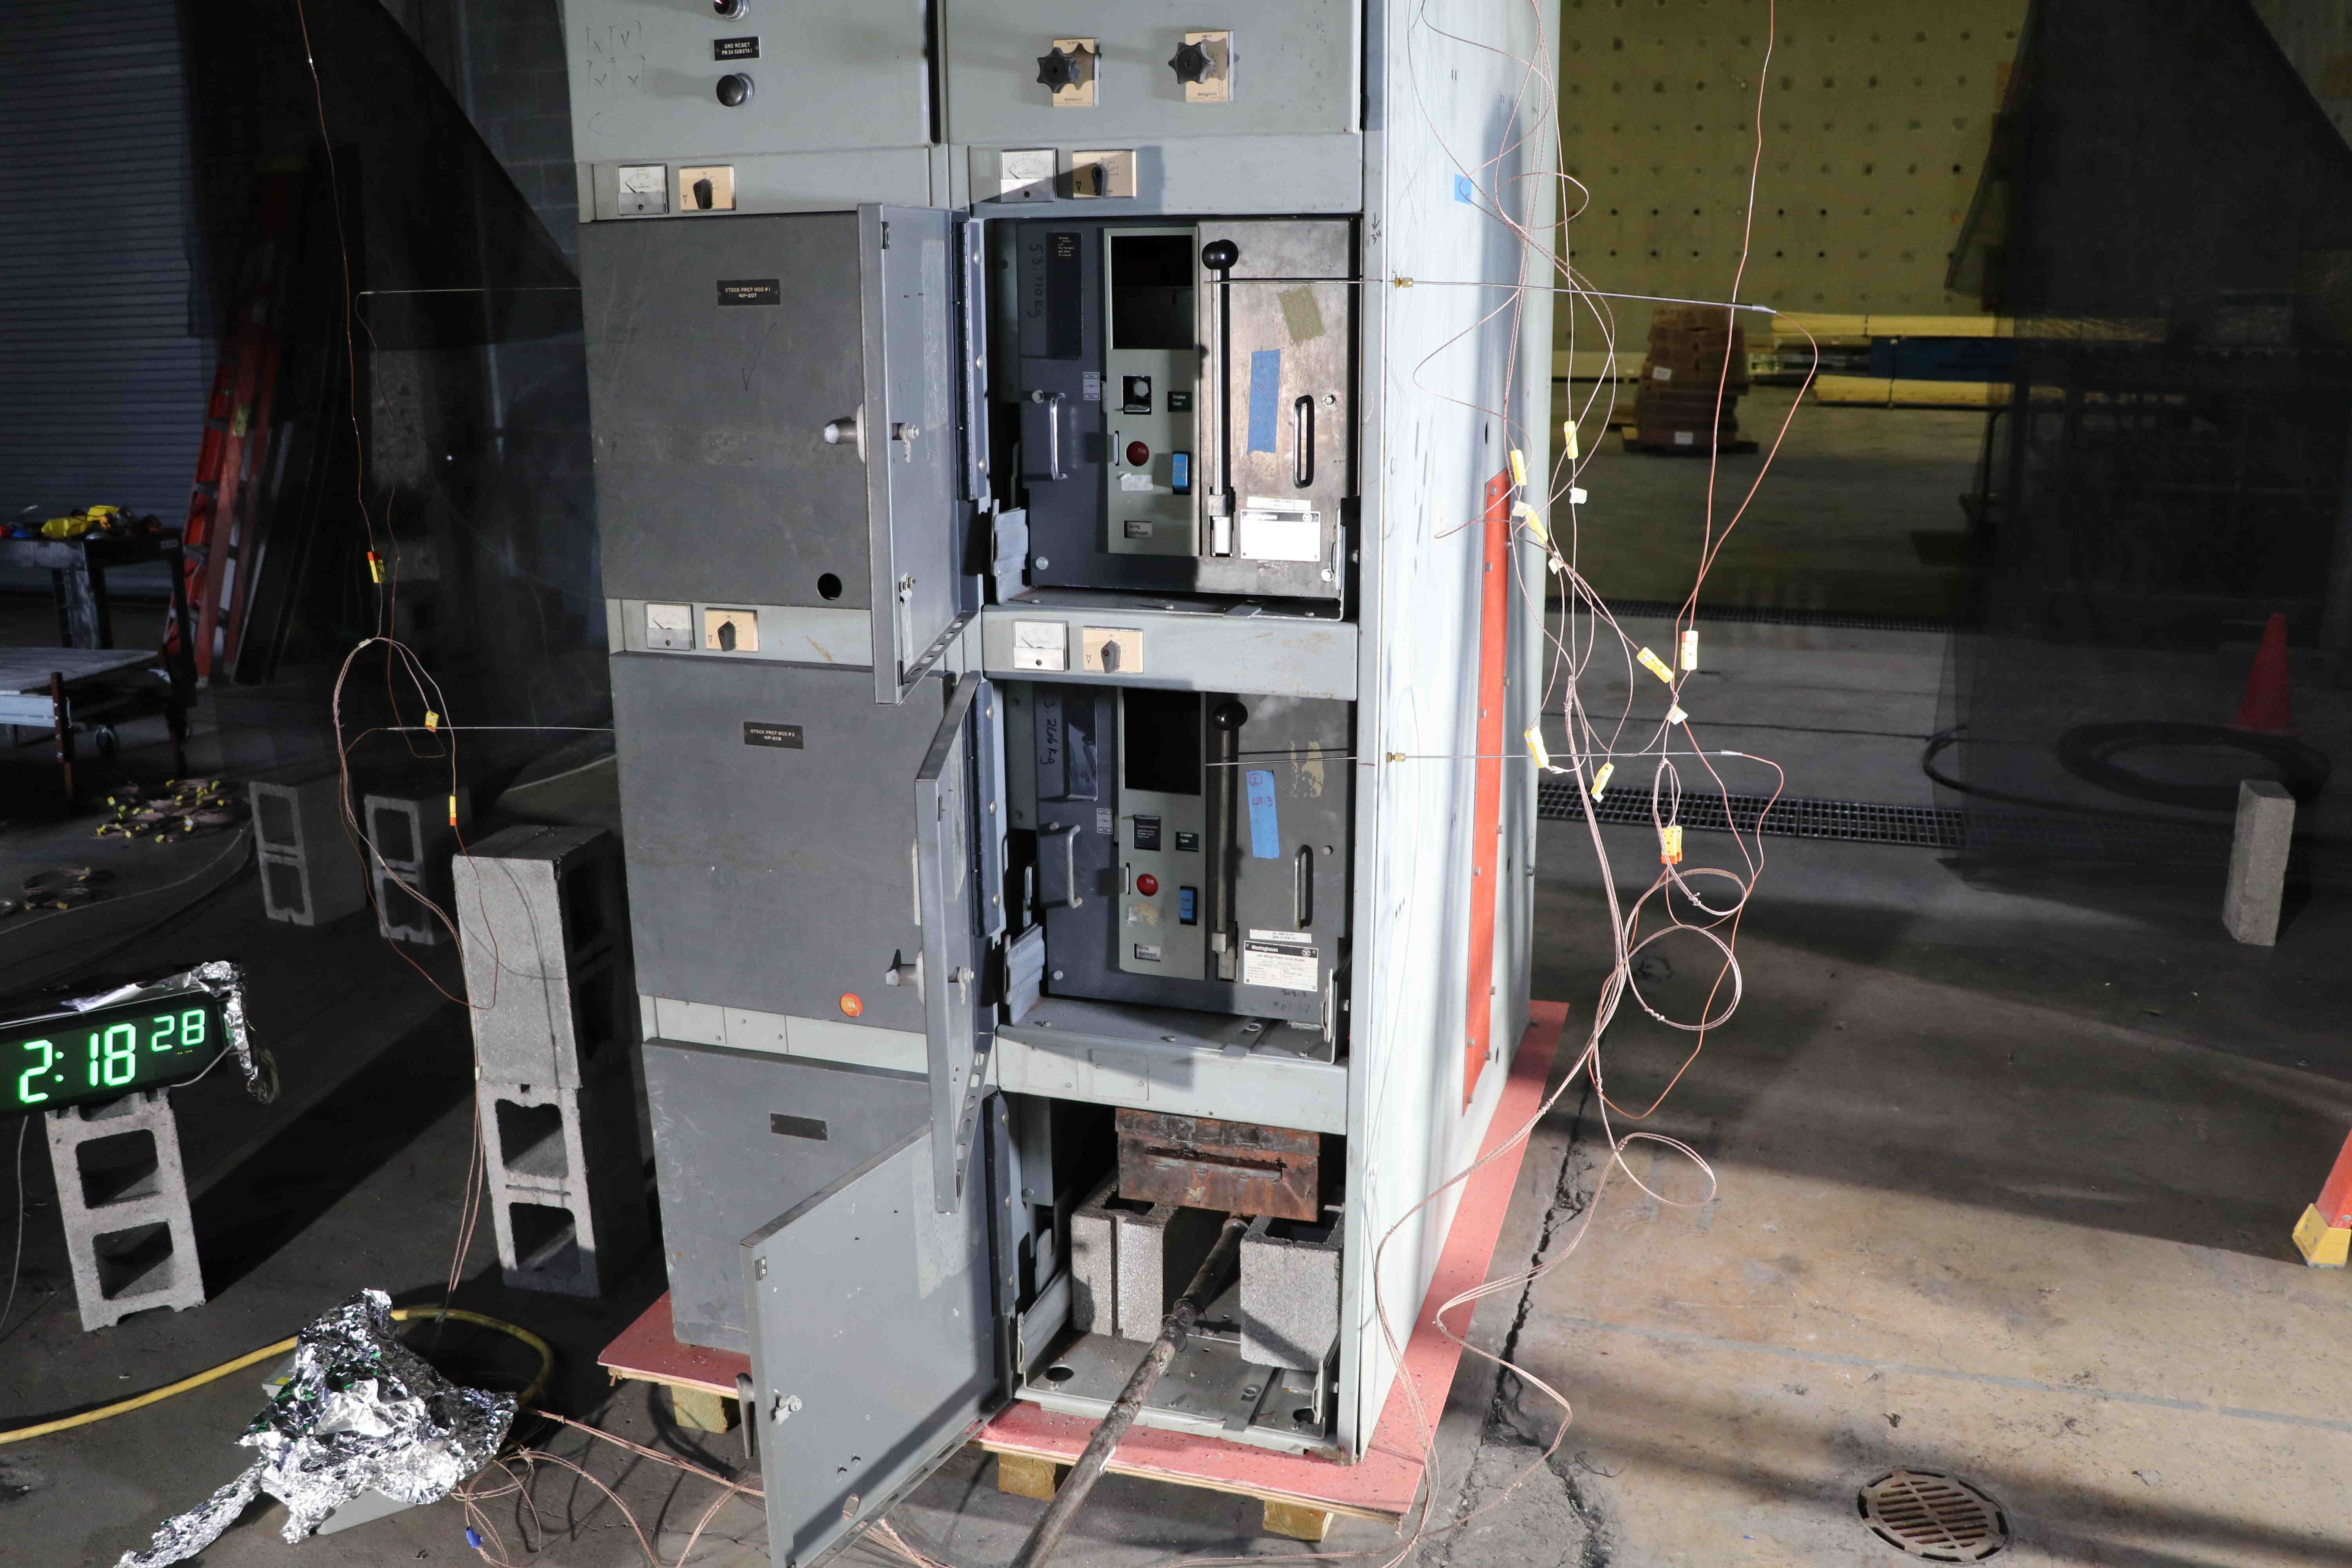
\includegraphics[height=2.75in]{../FIGURES/Test_40_setup} \\
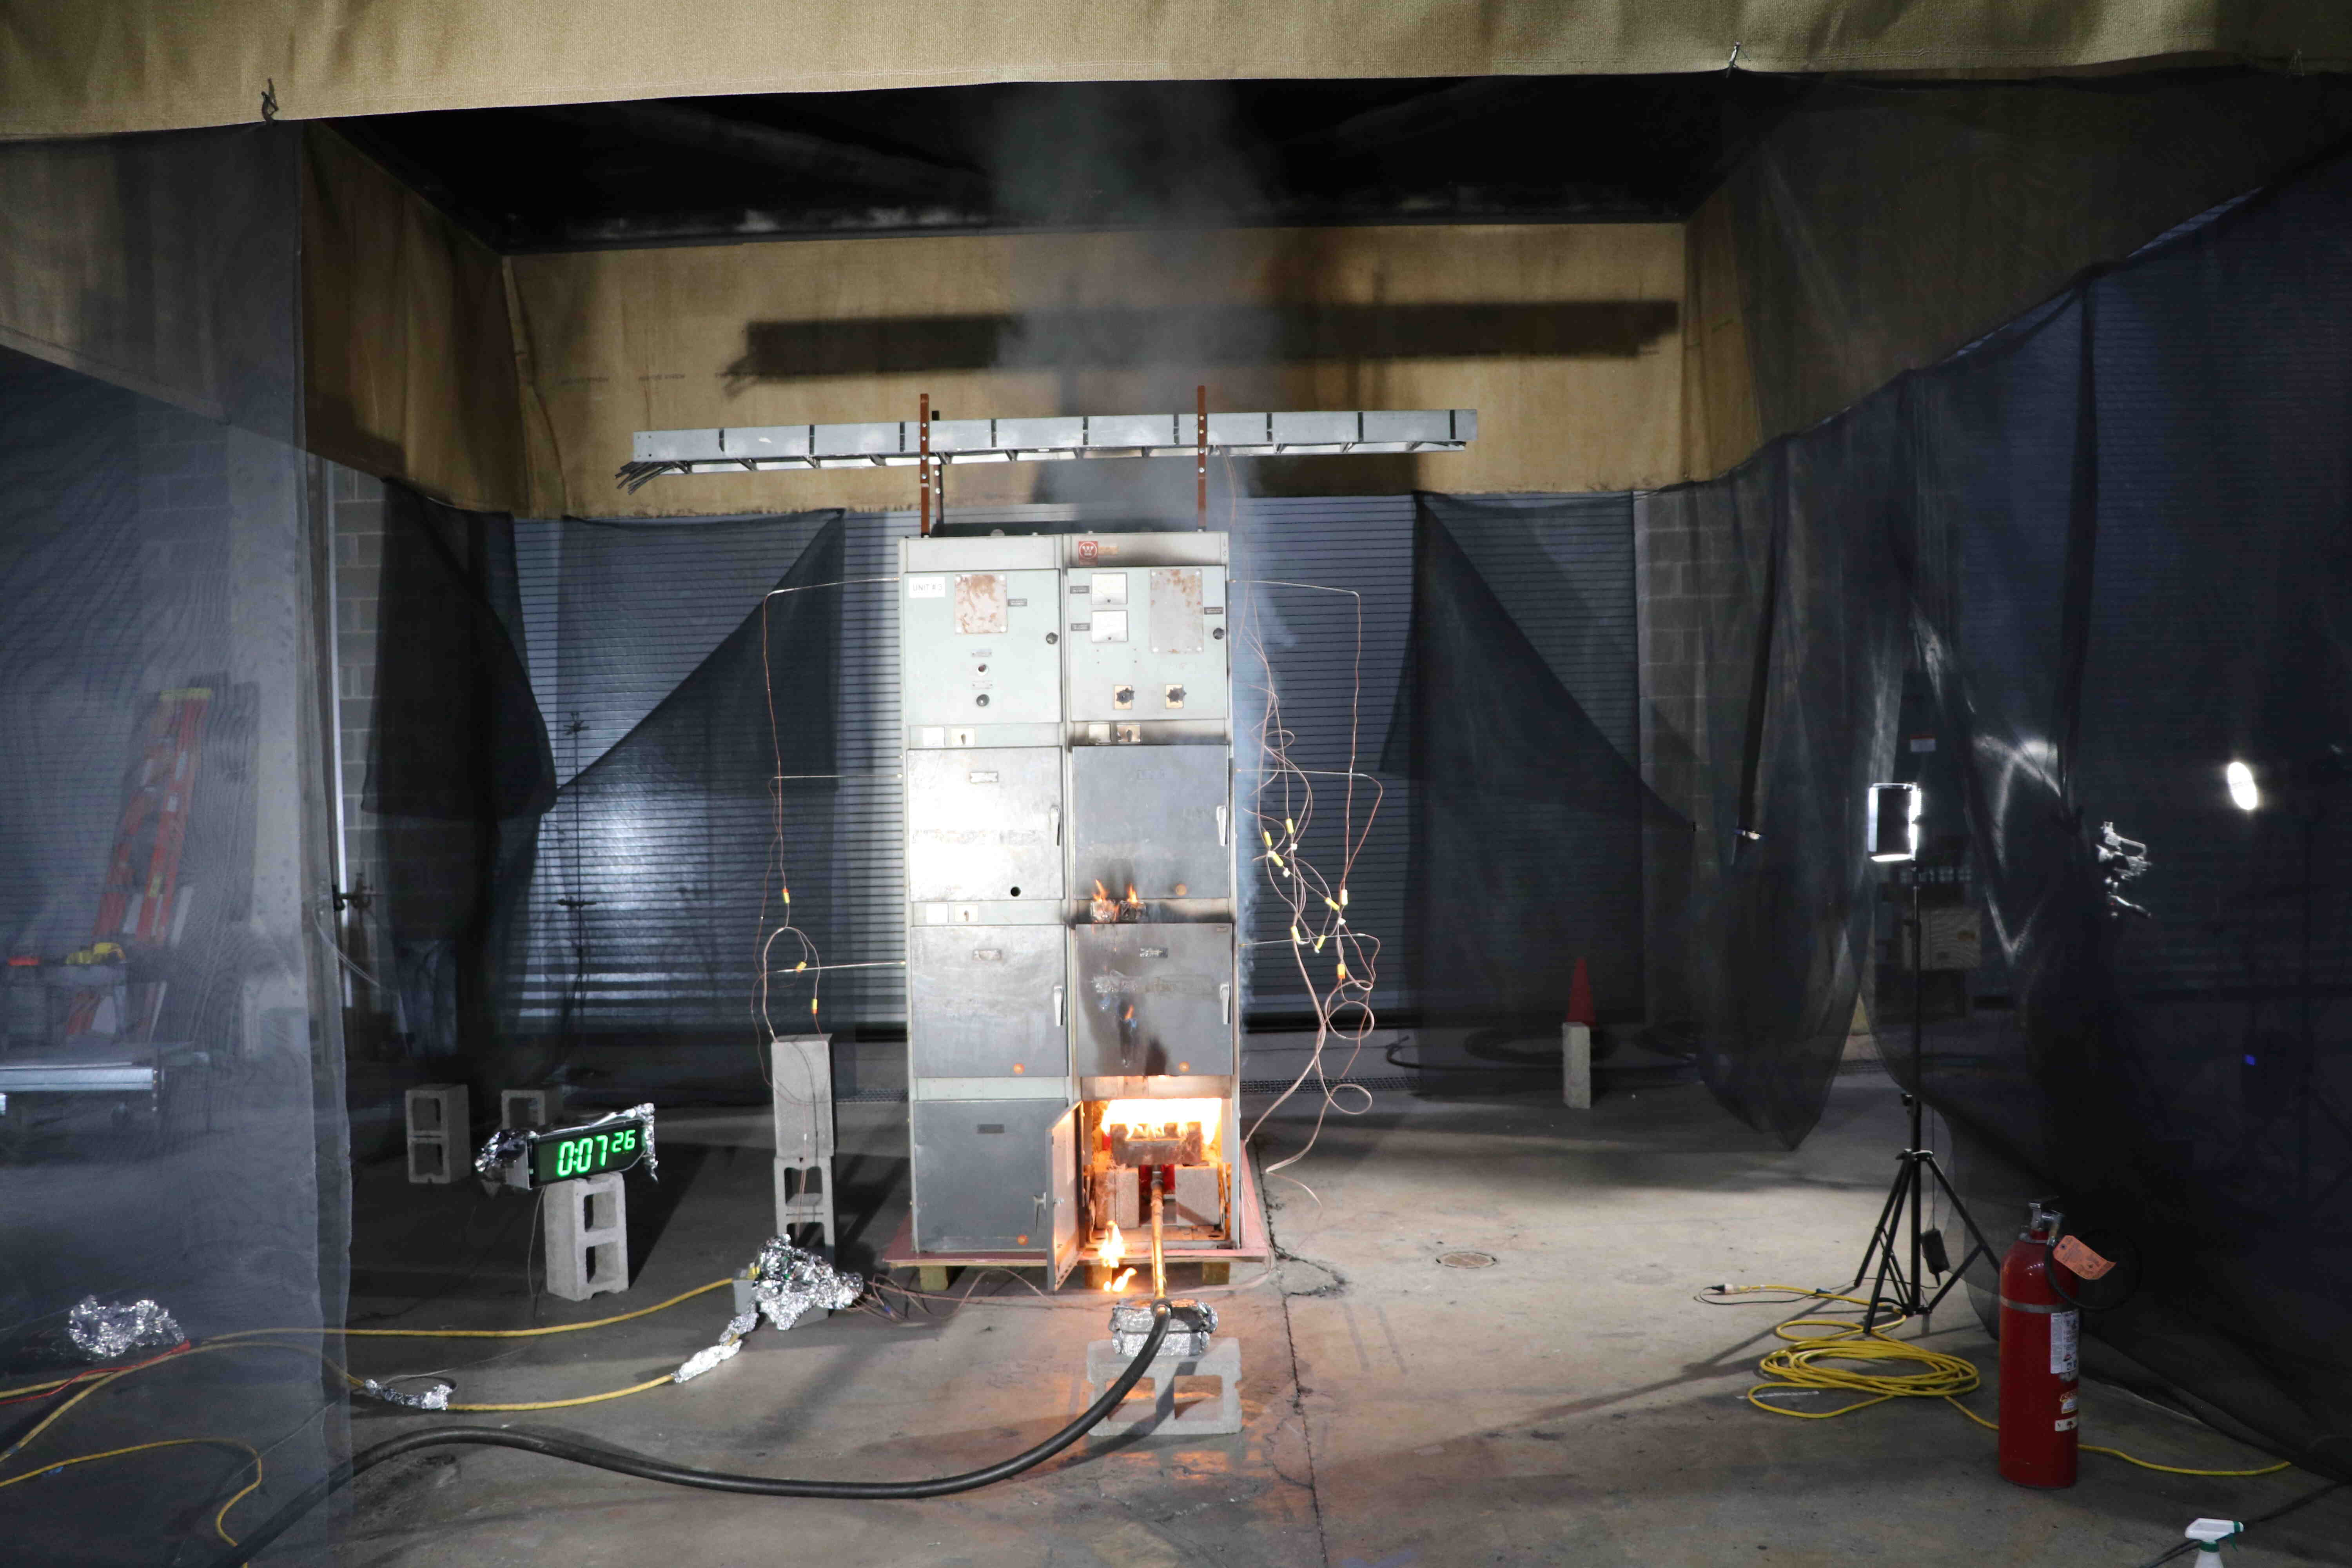
\includegraphics[height=2.75in]{../FIGURES/Test_40_7_min_26_s} \\
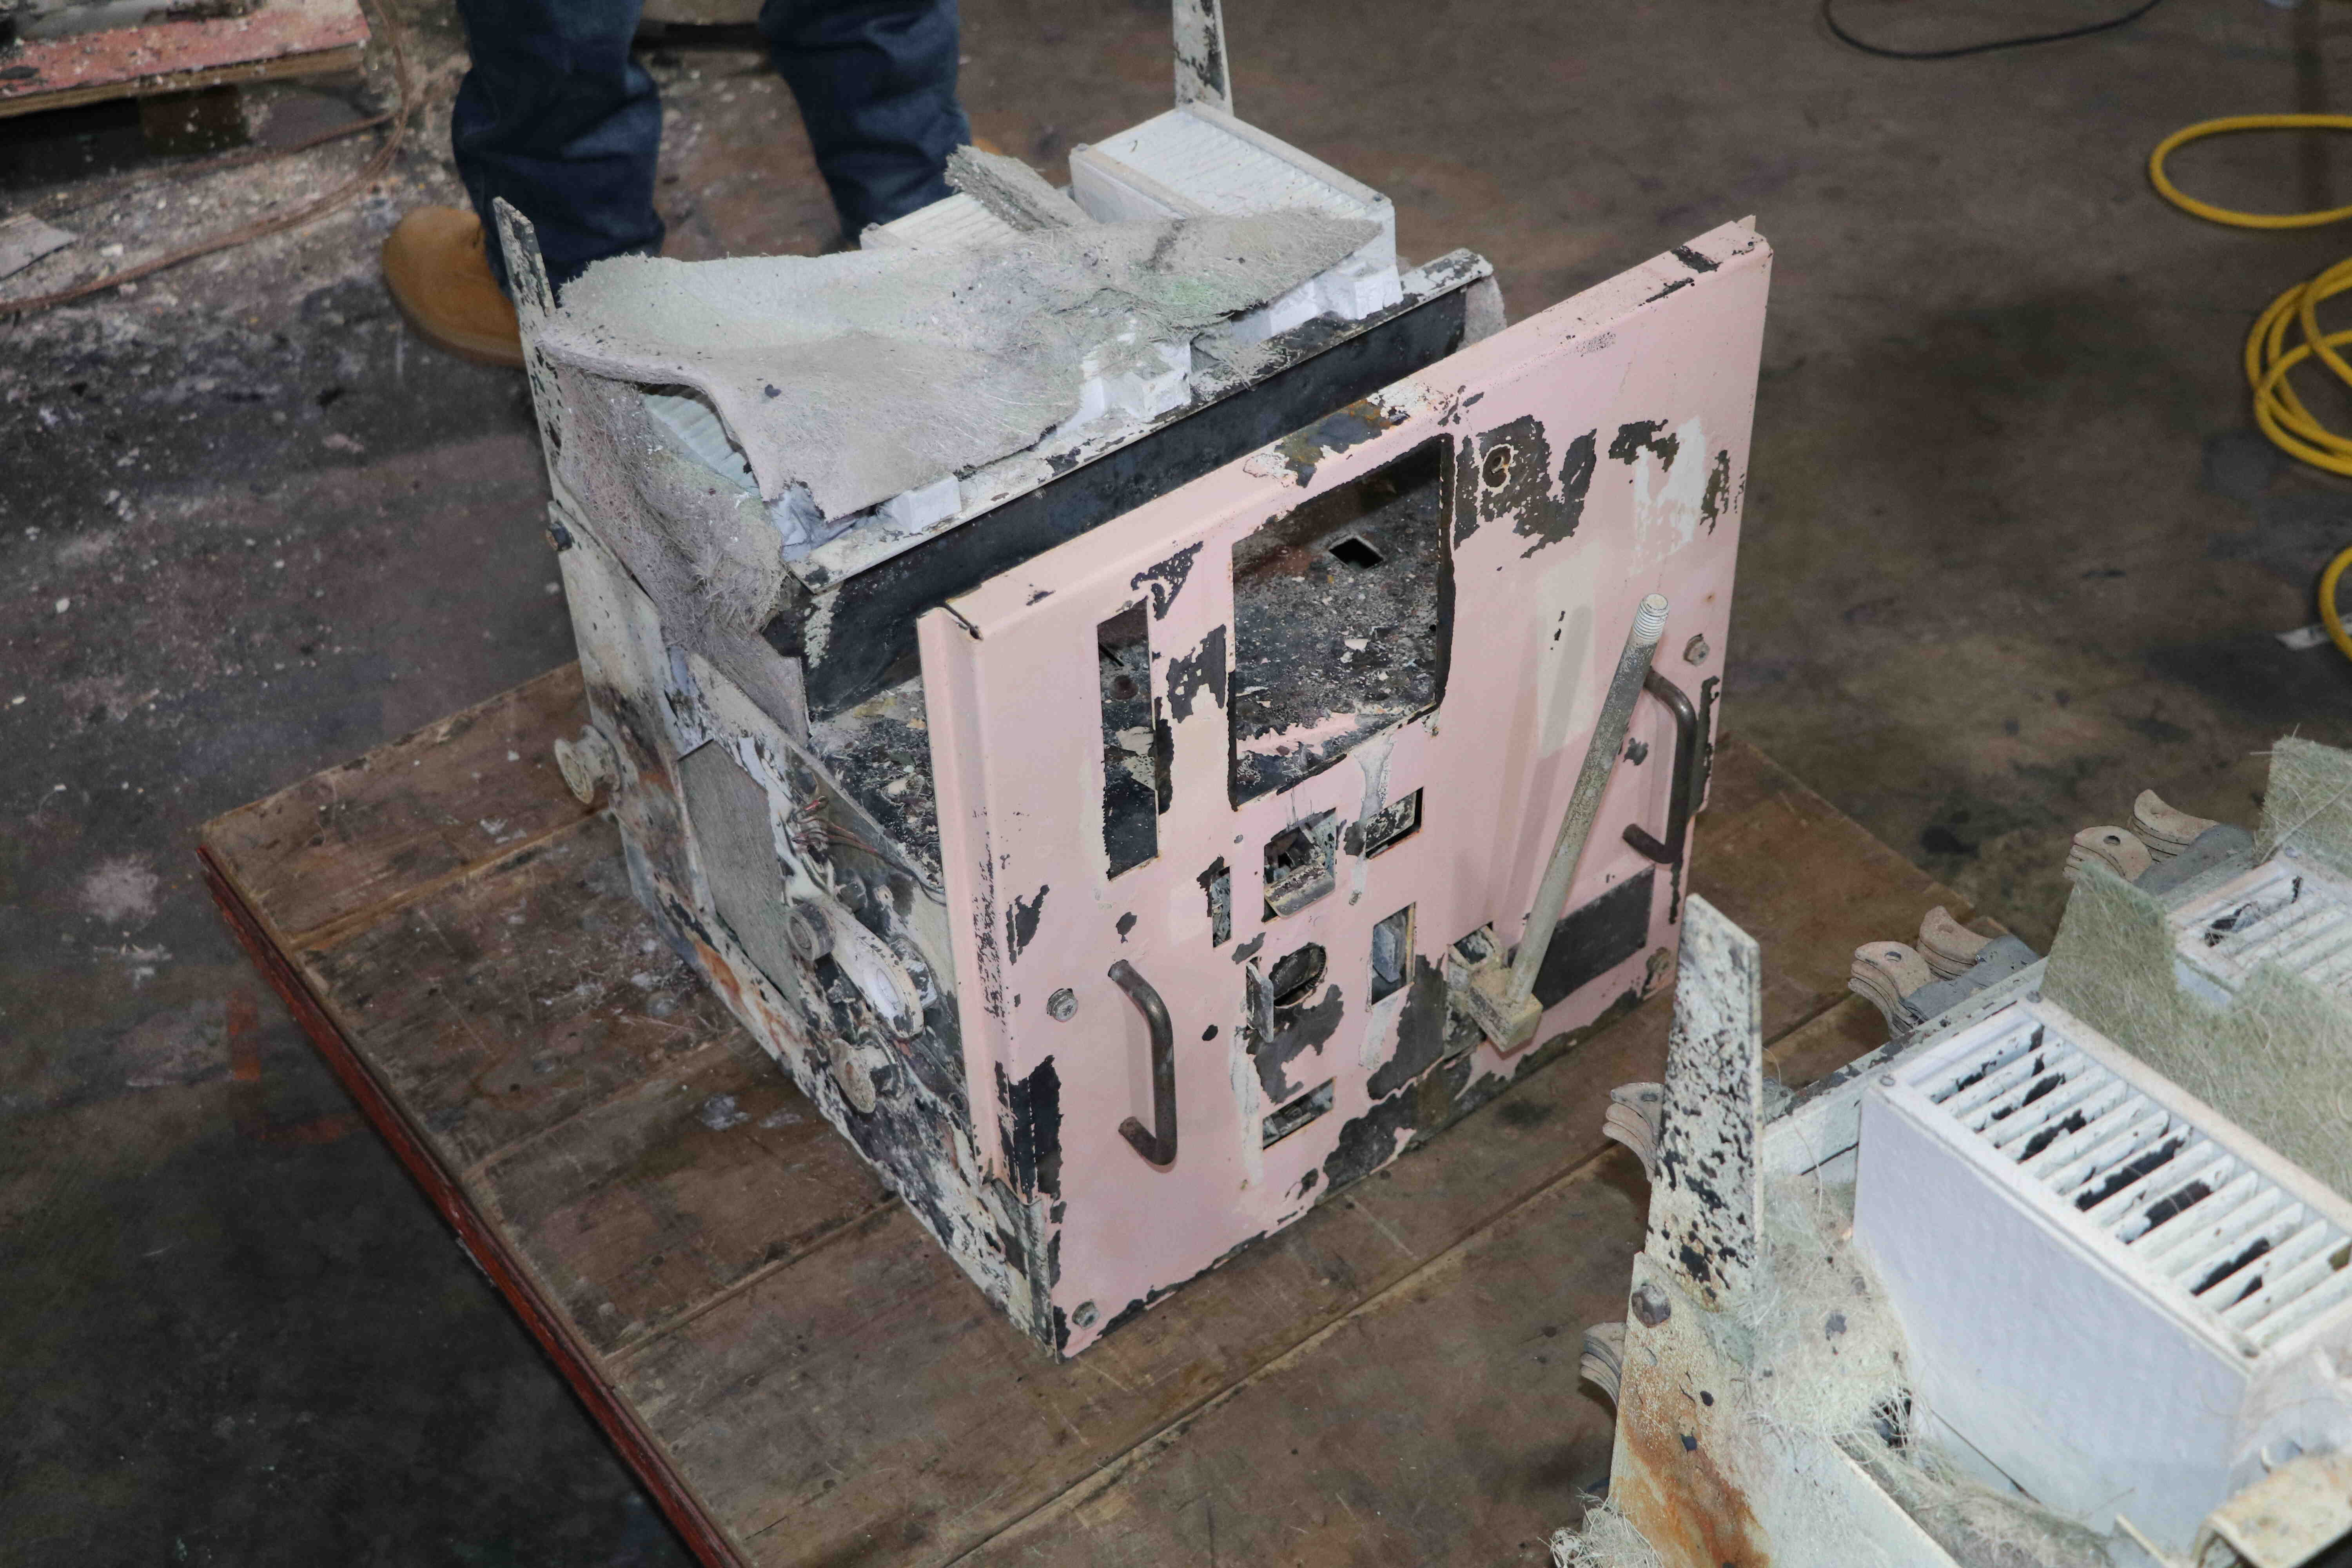
\includegraphics[height=2.75in]{../FIGURES/Test_40_breaker}
\caption[Photographs of Experiment~40]{Photographs of Experiment~40.}
\label{fig:Test_40_photos}
\end{figure}


\clearpage

\subsubsection{Experiment 41}

Referring to Fig.~\ref{fig:Test_41_photos}, the gas burner was positioned within the lower left compartment of a Westinghouse low voltage breaker enclosure. Breakers occupied the two compartments above, and the compartment above that was filled with approximately 1.0~kg of SIS wire. A 30~cm (12~in) wide tray containing 12 thermoplastic cables was placed approximately 30~cm (12~in) above the top of the enclosure. Thermocouples were inserted into three cables within the tray, and instrumented aluminum rods (``slugs'') were placed alongside the instrumented cables. A single sheathed thermocouple was placed at the front of each compartment. All doors on the left side of the enclosure remained open during the experiment.

The figures below show the heat release rate of the gas burner and the total heat release rate of the burner and cables, along with the internal temperatures of the cables and slugs.

\begin{figure}[!h]
\begin{tabular*}{\textwidth}{l@{\extracolsep{\fill}}r}
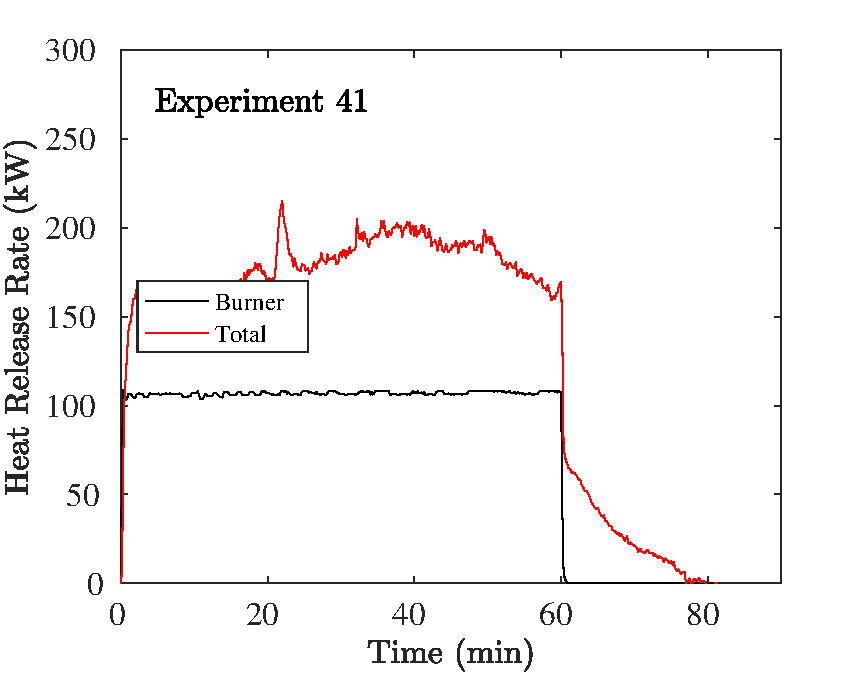
\includegraphics[height=2.65in]{../SCRIPT_FIGURES/Test_41_Plot_1} &
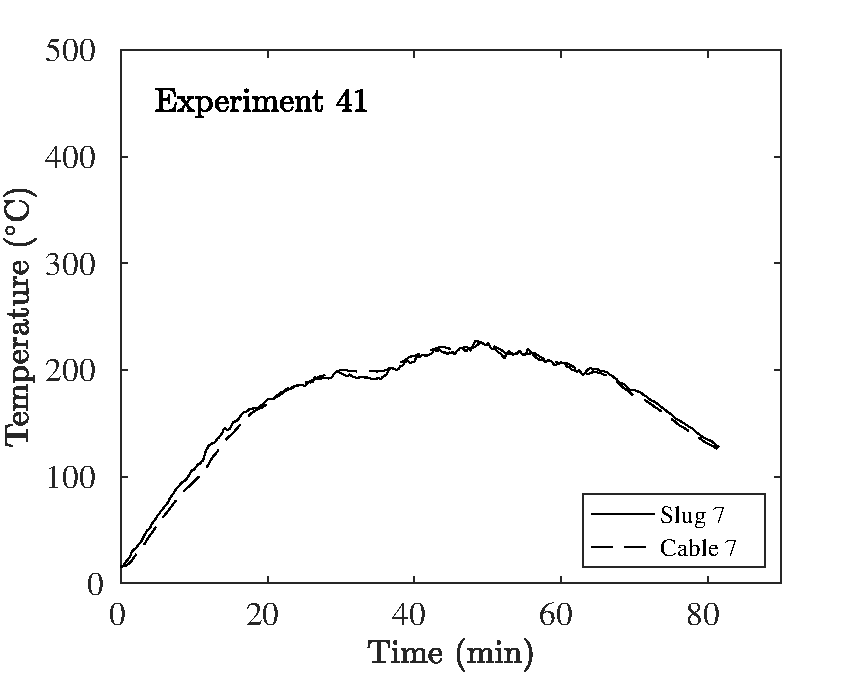
\includegraphics[height=2.65in]{../SCRIPT_FIGURES/Test_41_Plot_2} \\
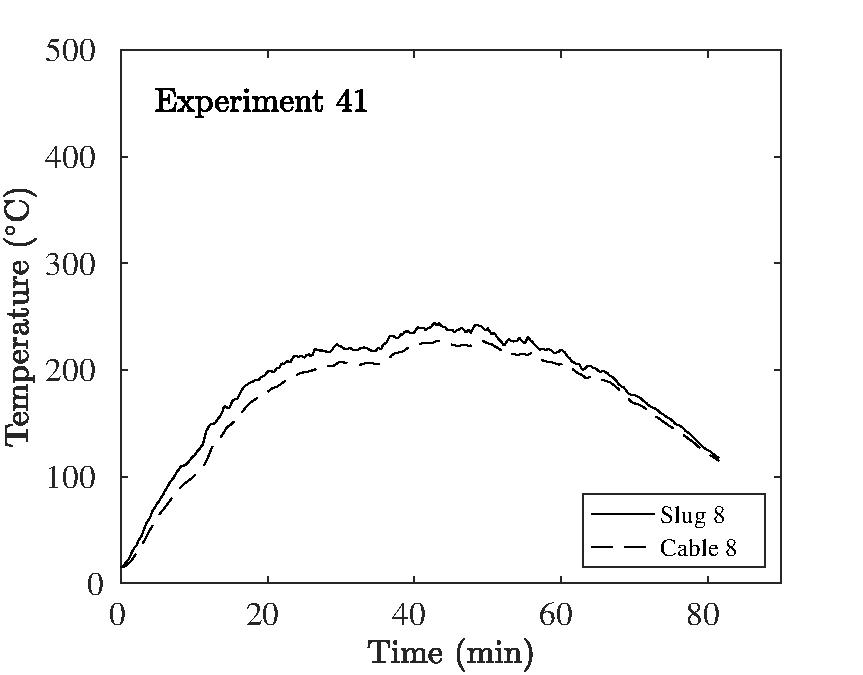
\includegraphics[height=2.65in]{../SCRIPT_FIGURES/Test_41_Plot_3} &
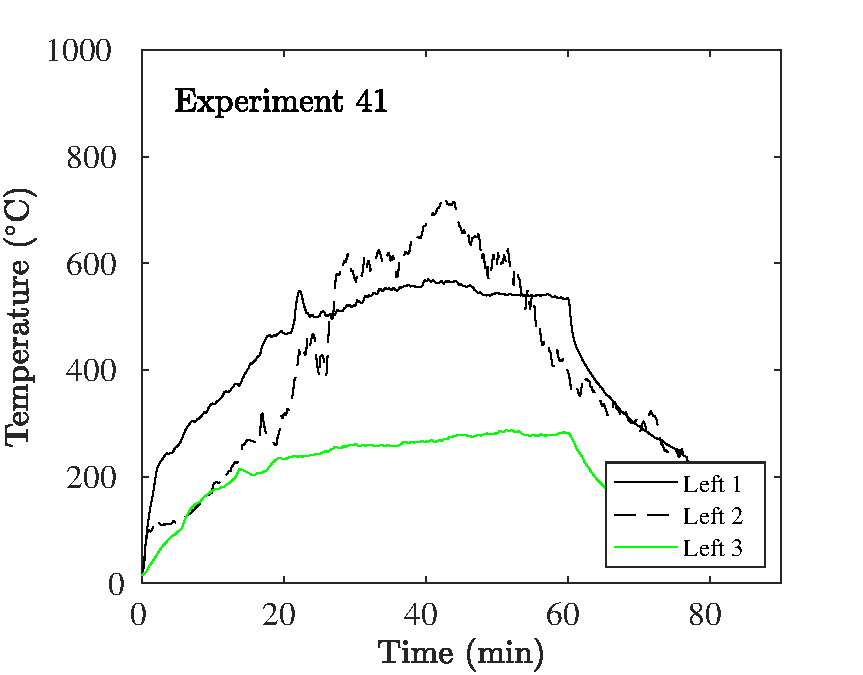
\includegraphics[height=2.65in]{../SCRIPT_FIGURES/Test_41_Plot_5}
\end{tabular*}
\caption[HRR and temperatures of Experiment 41]{Heat release rate (upper left) and various temperatures inside and above a burning breaker enclosure.}
\label{fig:Test_41}
\end{figure}

\begin{figure}[p]
\centering
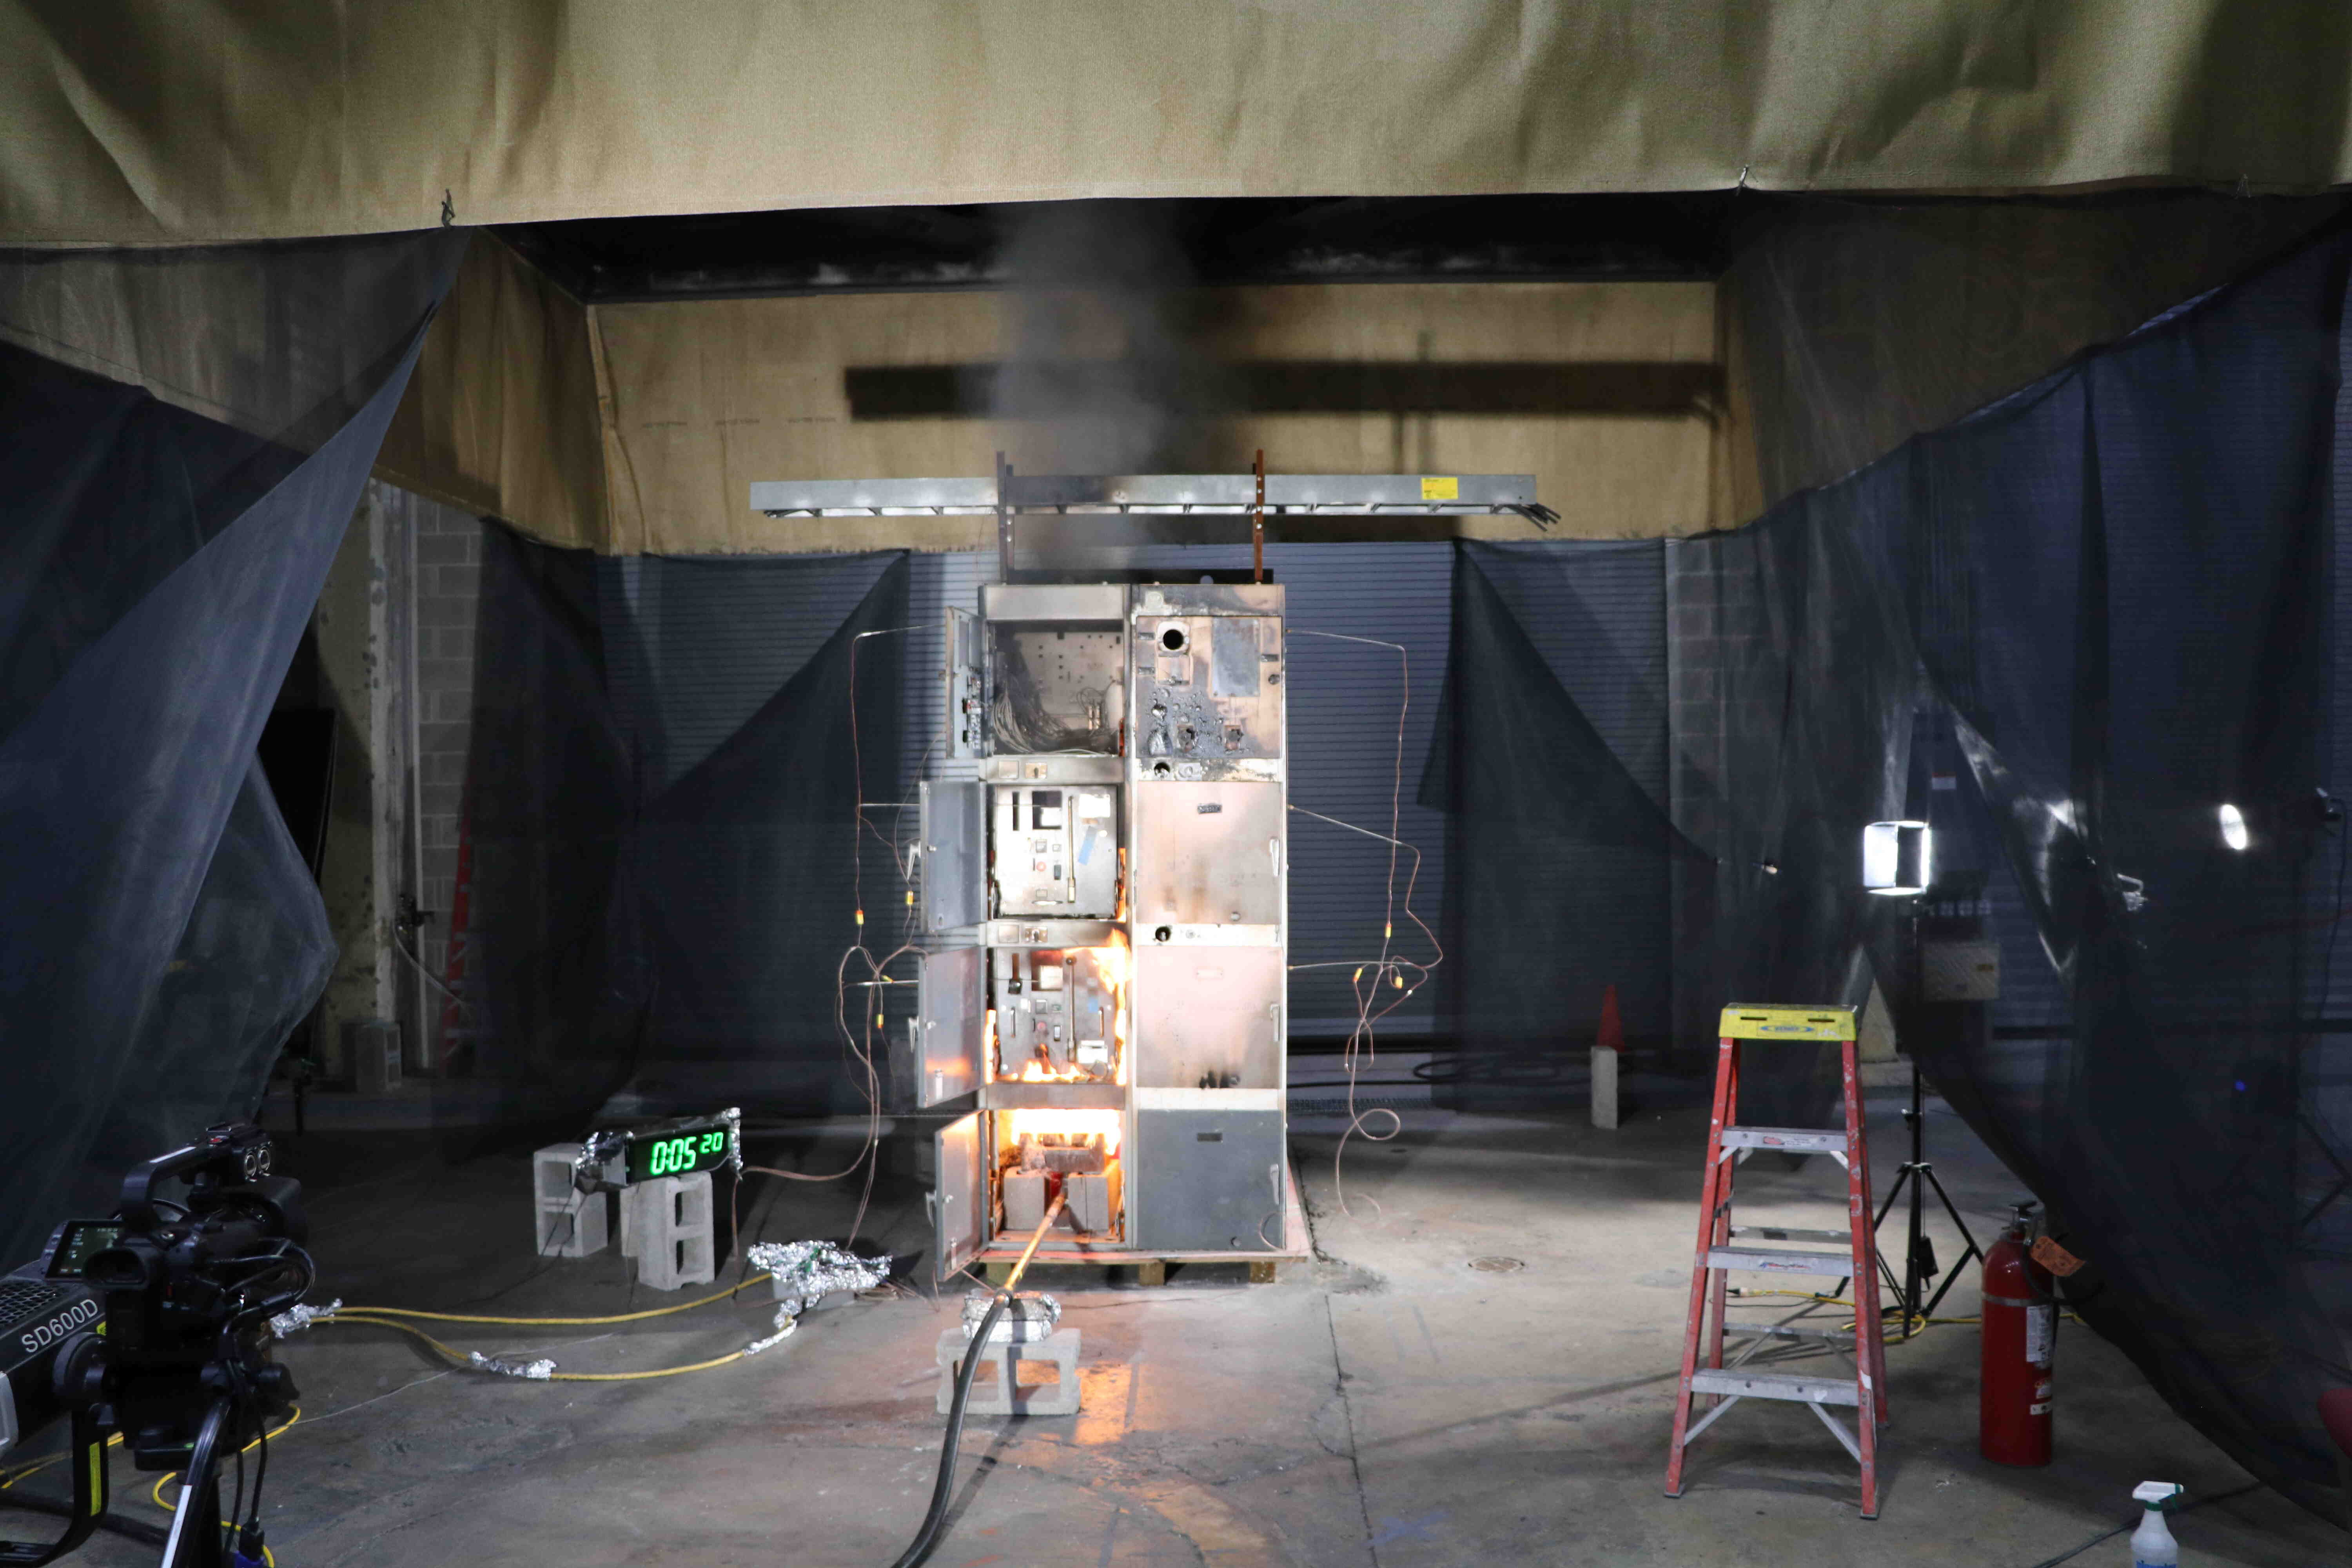
\includegraphics[height=2.75in]{../FIGURES/Test_41_5_min_20_s} \\
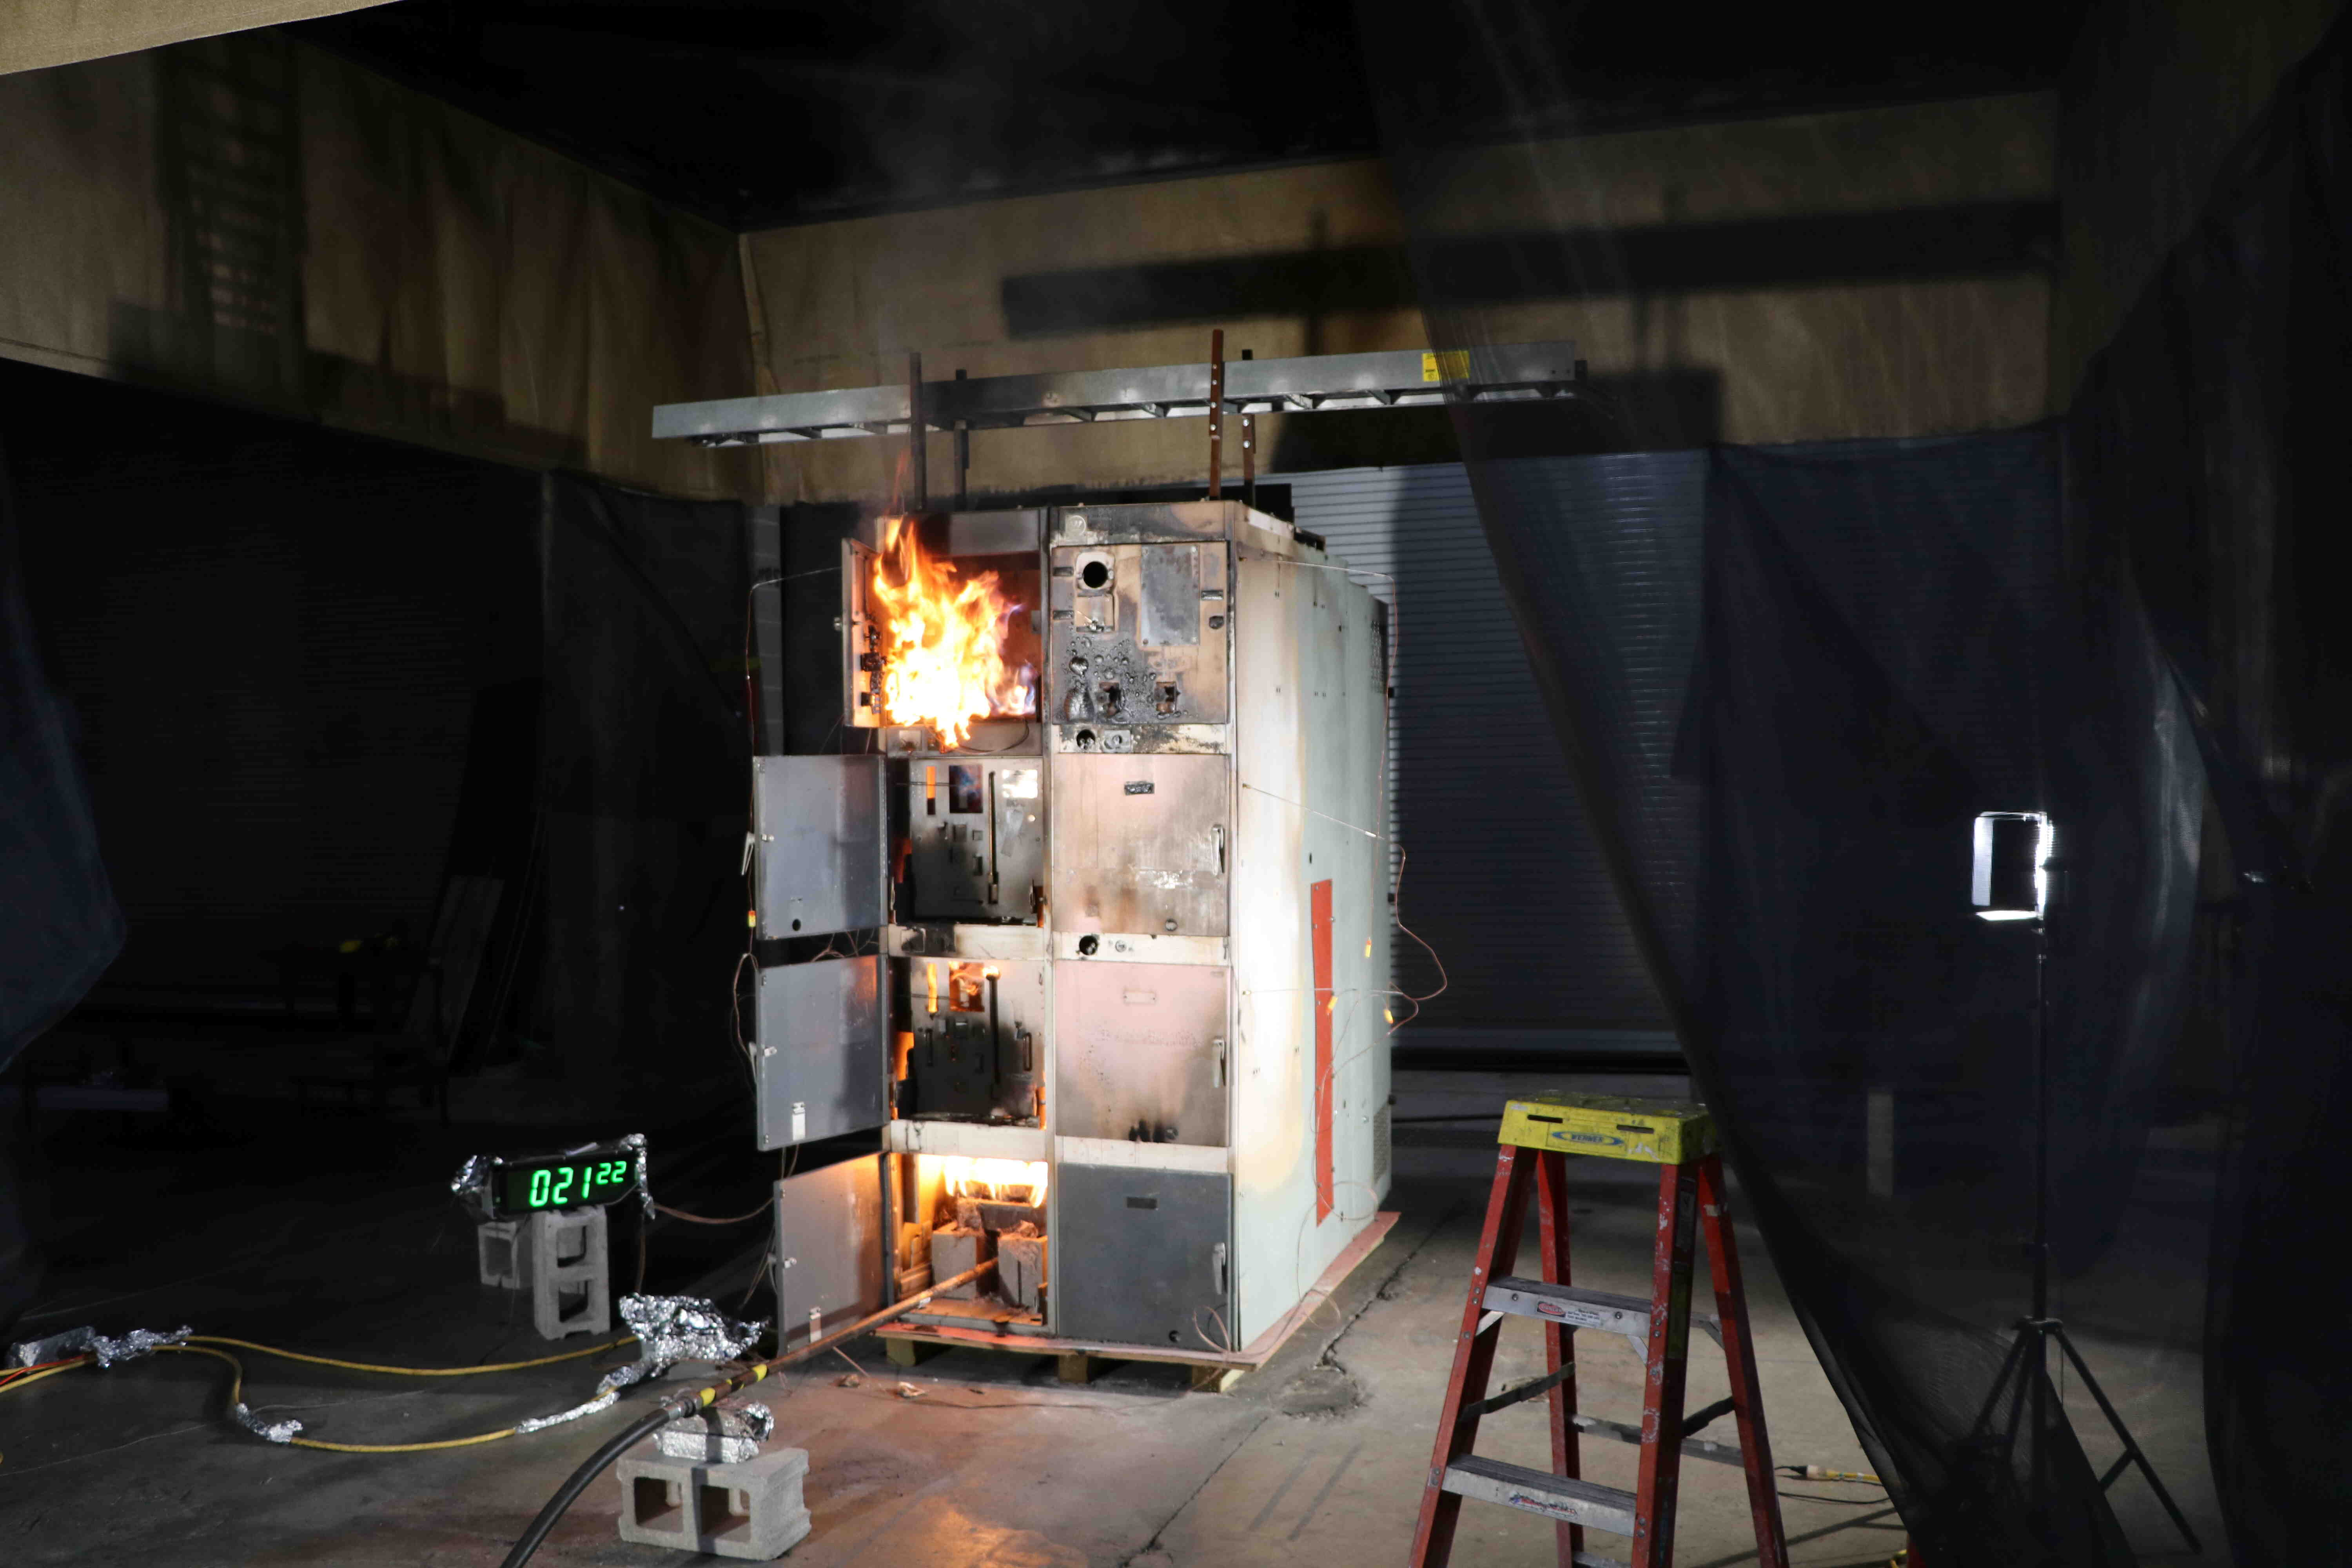
\includegraphics[height=2.75in]{../FIGURES/Test_41_21_min_22_s} \\
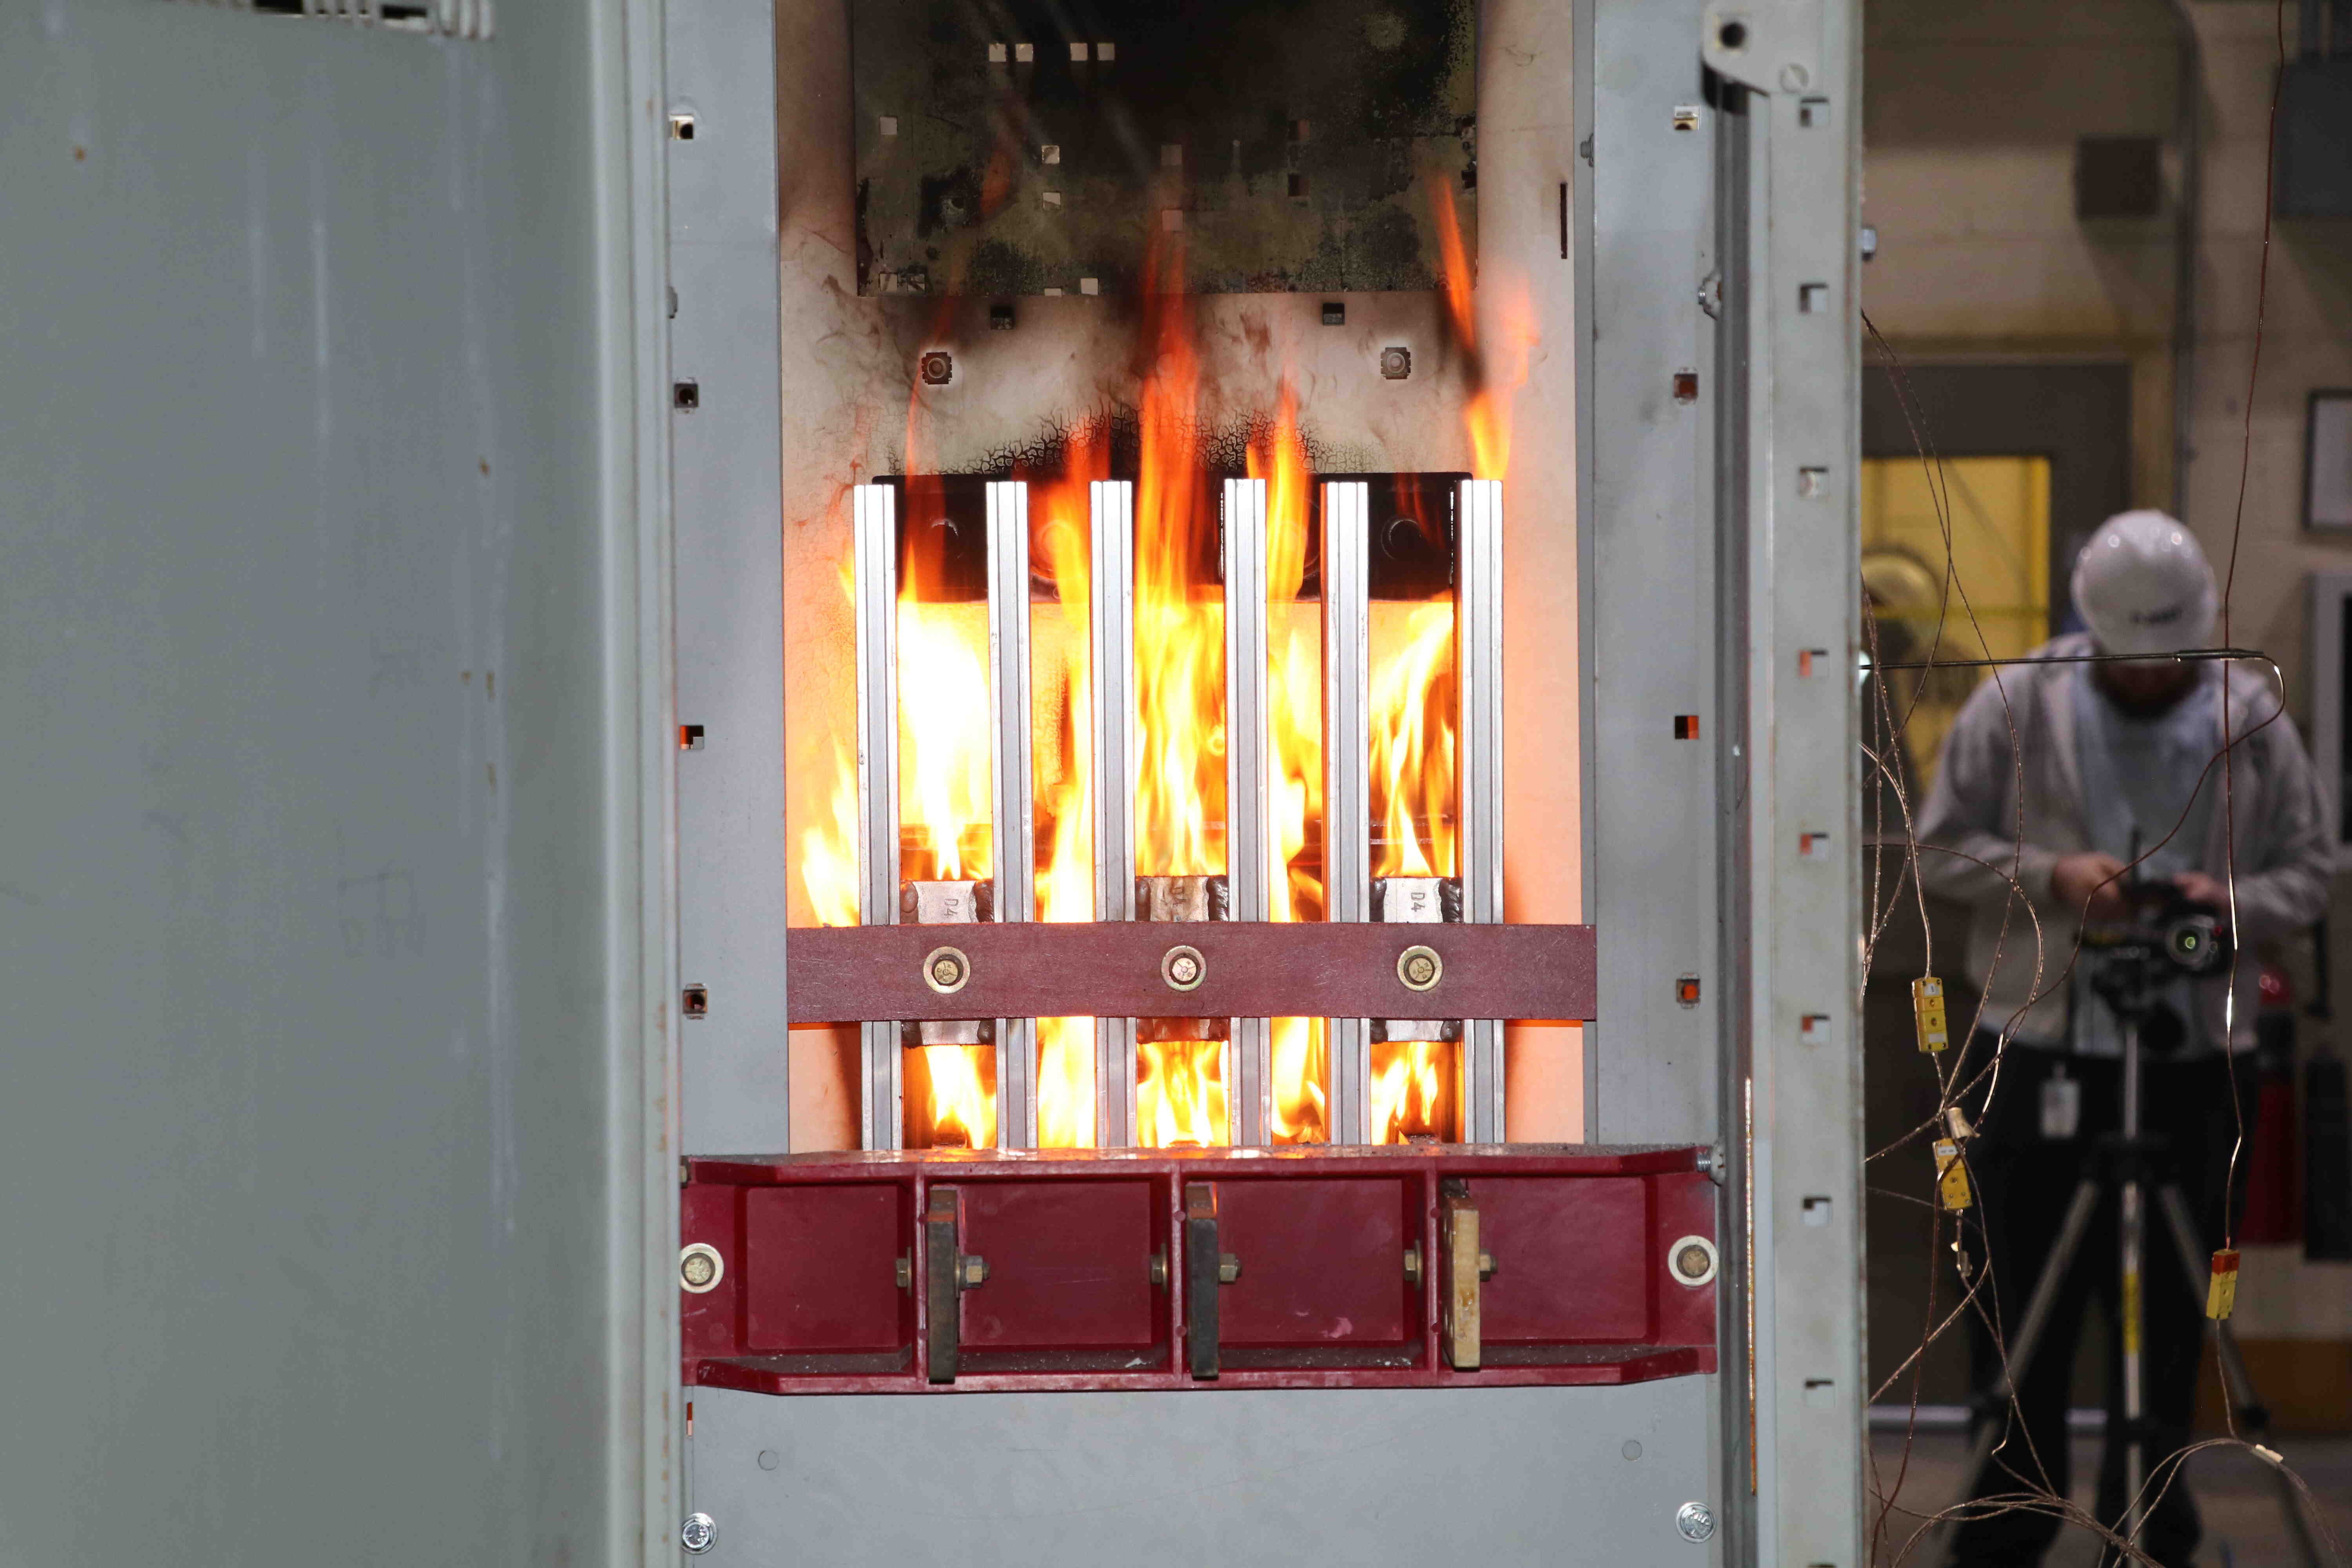
\includegraphics[height=2.75in]{../FIGURES/Test_41_rear}
\caption[Photographs of Experiment~41]{Photographs of Experiment~41.}
\label{fig:Test_41_photos}
\end{figure}






\clearpage

\section{Thermal Exposure of Cables Above a Burning Electrical Enclosure}

Three types of experiments were conducted to assess the thermal exposure of electrical cables above a burning enclosure:
\begin{enumerate}
\item Single trays of cables were positioned above a gas burner.
\item Plume temperatures were measured above vents in a burning electrical enclosure.
\item Cable trays were exposed to fire plumes above burning enclosures.
\end{enumerate}
Two types of cables were used in these experiments. The one referred to as the ``thermoplastic'' cable has polyethylene insulation covering its seven 12~AWG\footnote{American Wire Gauge} copper conductors. Its jacket is approximately 1.9~mm thick polyvinyl chloride (PVC). The cable is approximately 15.9~mm (0.63~in) in diameter and has a mass of 0.38~kg/m. It is approximately 55~\% by mass copper, 27~\% jacket, 10~\% insulation, and 8~\% filler.

The cable referred to as the ``thermoset'' has cross-linked polyethylene insulation covering its twelve 18~AWG copper conductors. Its jacket is approximately 1.5~mm thick chlorosulfonated polyethylene (CSPE). The cable is approximately 12.7~mm (0.5~in) in diameter and has a mass of 0.25~kg/m. It is approximately 37~\% by mass copper, 33~\% jacket, 29~\% insulation, and 1~\% filler.

\subsection{Single Tray Ignition Study}

In these experiments, a single 45~cm (18~in) wide tray containing either thermoplastic or thermoset cables was positioned above a 30~cm (12~in) square natural gas burner with a heat release rate of approximately 40~kW. Some of the cables had Type-K thermocouple embedded with an aluminum rod (``slug'') positioned alongside. The purpose of the experiments was two-fold: (1) to correlate internal cable temperature with ignition time, and (2) to assess the use of the aluminum slugs as a surrogate for actual cables in testing of this sort.



\clearpage

\subsubsection{Experiment 36}

A 45~cm (18~in) wide tray containing 13 thermoplastic cables (\#900) was placed approximately 36~cm (14~in) above a nominally 30~cm square 40~kW natural gas burner. Thermocouples were inserted into three cables above the burner, and instrumented aluminum rods (``slugs'') were placed alongside the instrumented cables. The figures below show the heat release rate of the gas burner and the total heat release rate of the burner and cables, along with the internal temperatures of the cables and slugs. The cable ignited at approximately 3~min.

\begin{figure}[!h]
\begin{tabular*}{\textwidth}{l@{\extracolsep{\fill}}r}
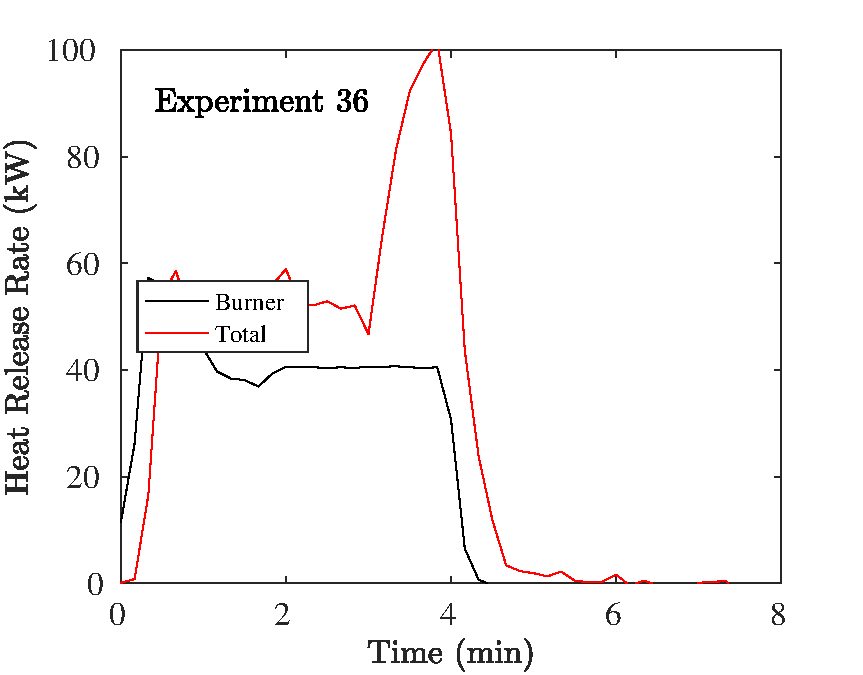
\includegraphics[height=2.65in]{../SCRIPT_FIGURES/Test_36_Plot_1} &
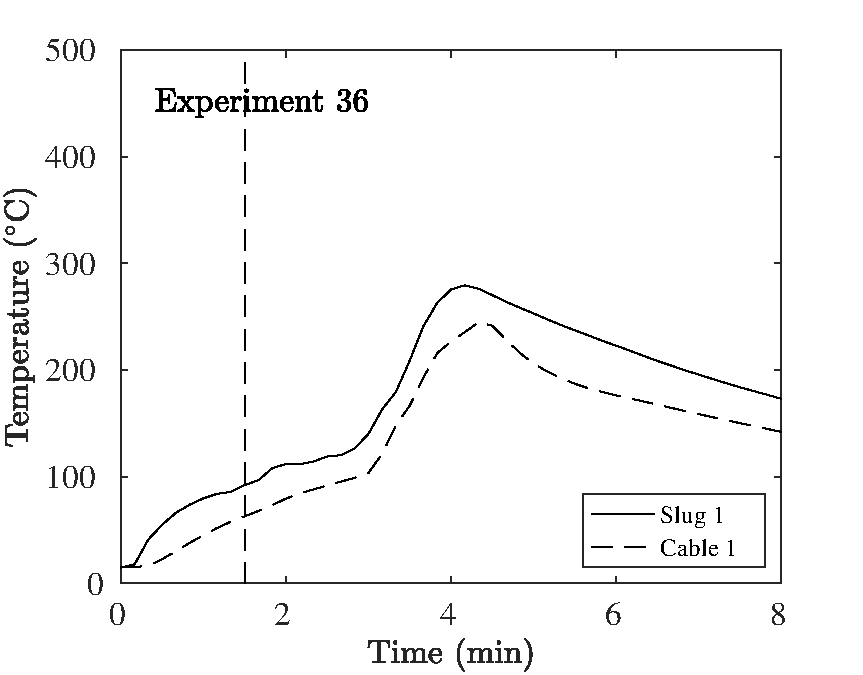
\includegraphics[height=2.65in]{../SCRIPT_FIGURES/Test_36_Plot_2} \\
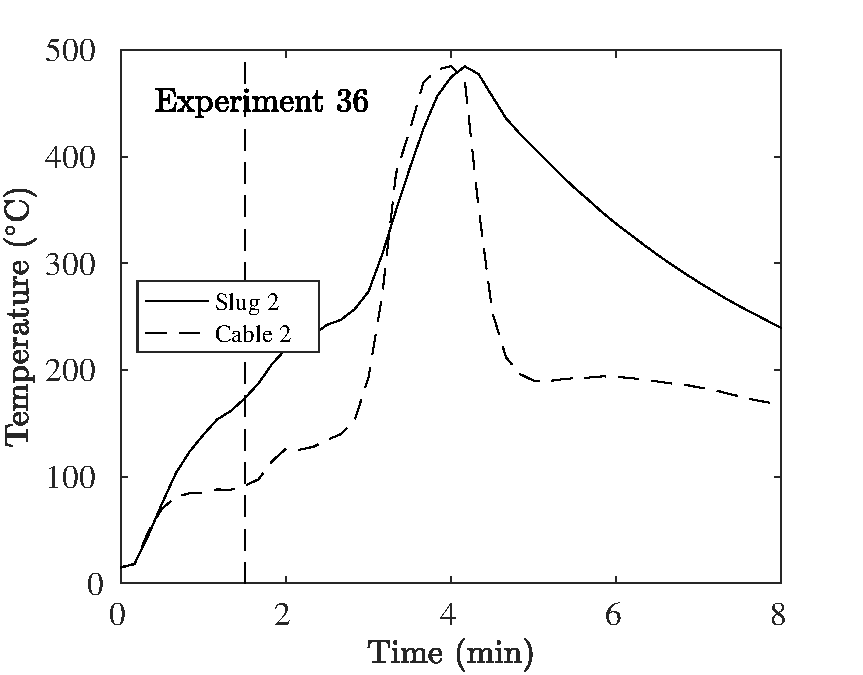
\includegraphics[height=2.65in]{../SCRIPT_FIGURES/Test_36_Plot_3} &
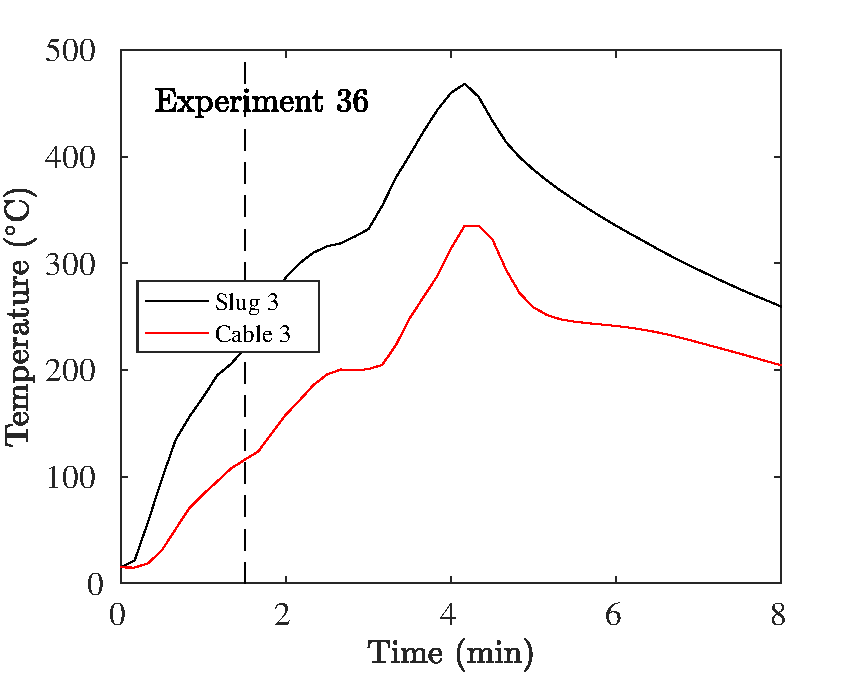
\includegraphics[height=2.65in]{../SCRIPT_FIGURES/Test_36_Plot_4}
\end{tabular*}
\caption[HRR and temperatures of Experiment 36]{Heat release rate (upper left) and internal cable and slug temperatures above a 40~kW burner. The vertical dashed line indicates cable ignition.}
\label{fig:Test_36}
\end{figure}

\begin{figure}[p]
\centering
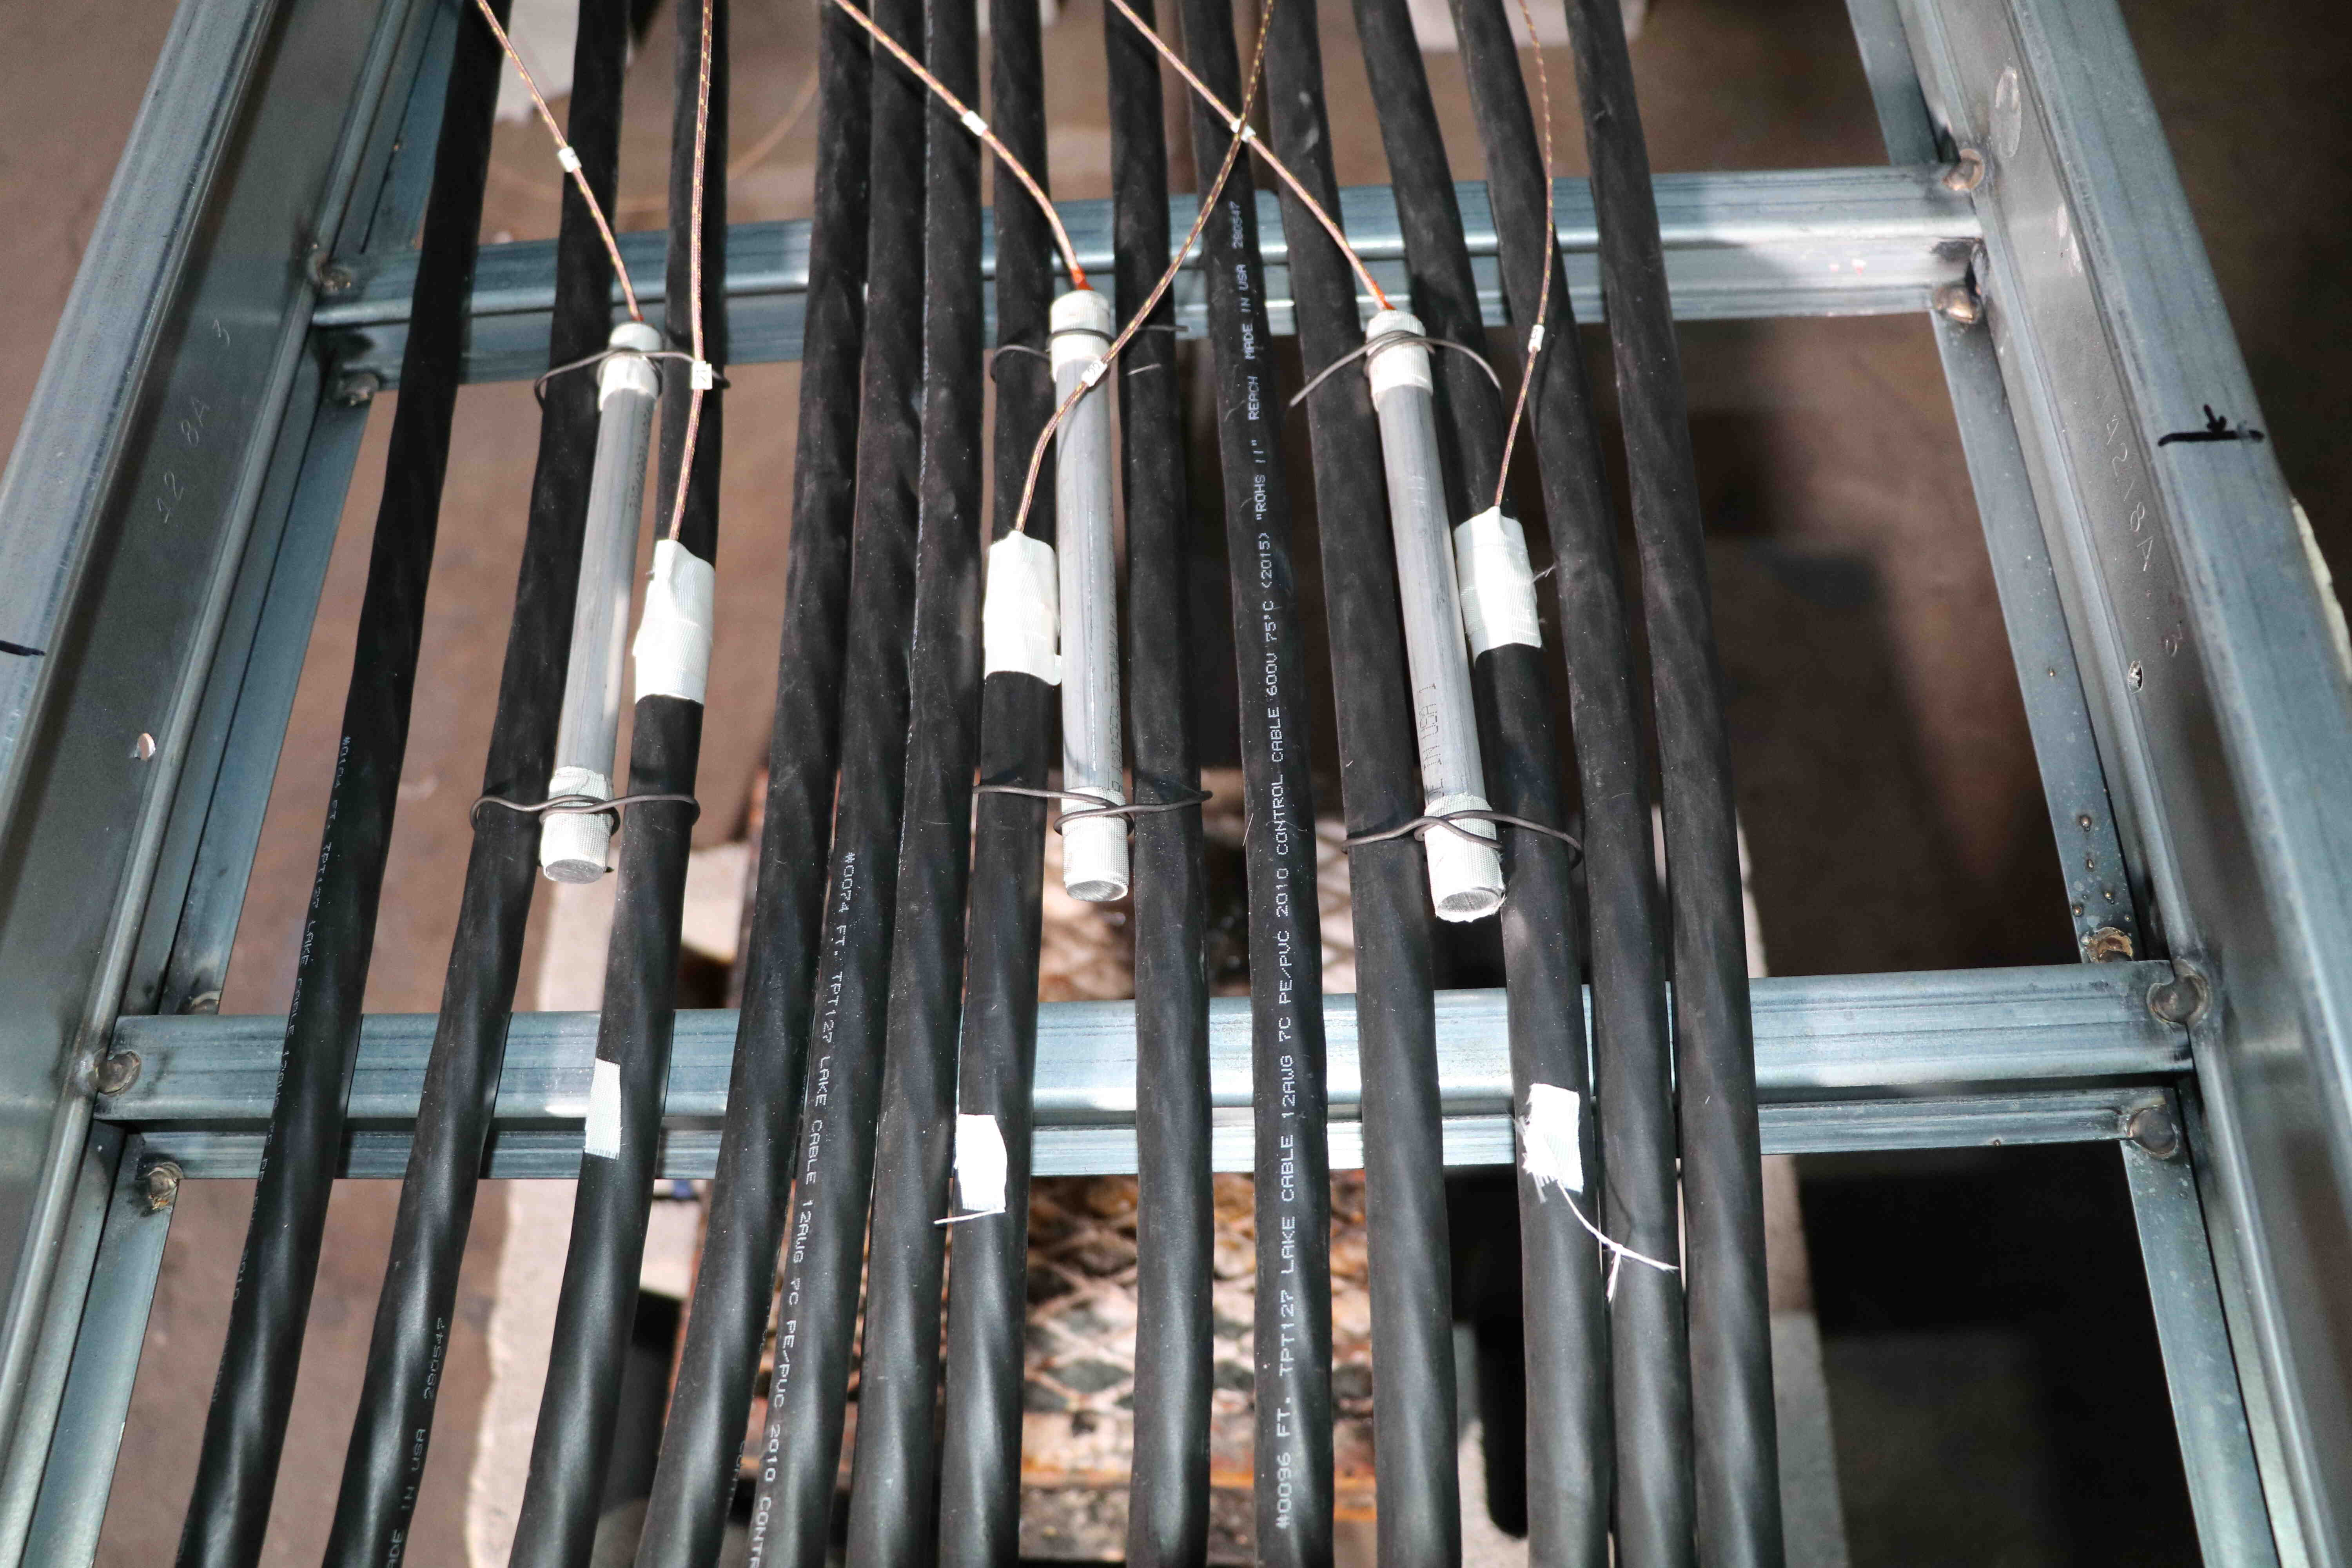
\includegraphics[height=2.75in]{../FIGURES/Test_36_setup} \\
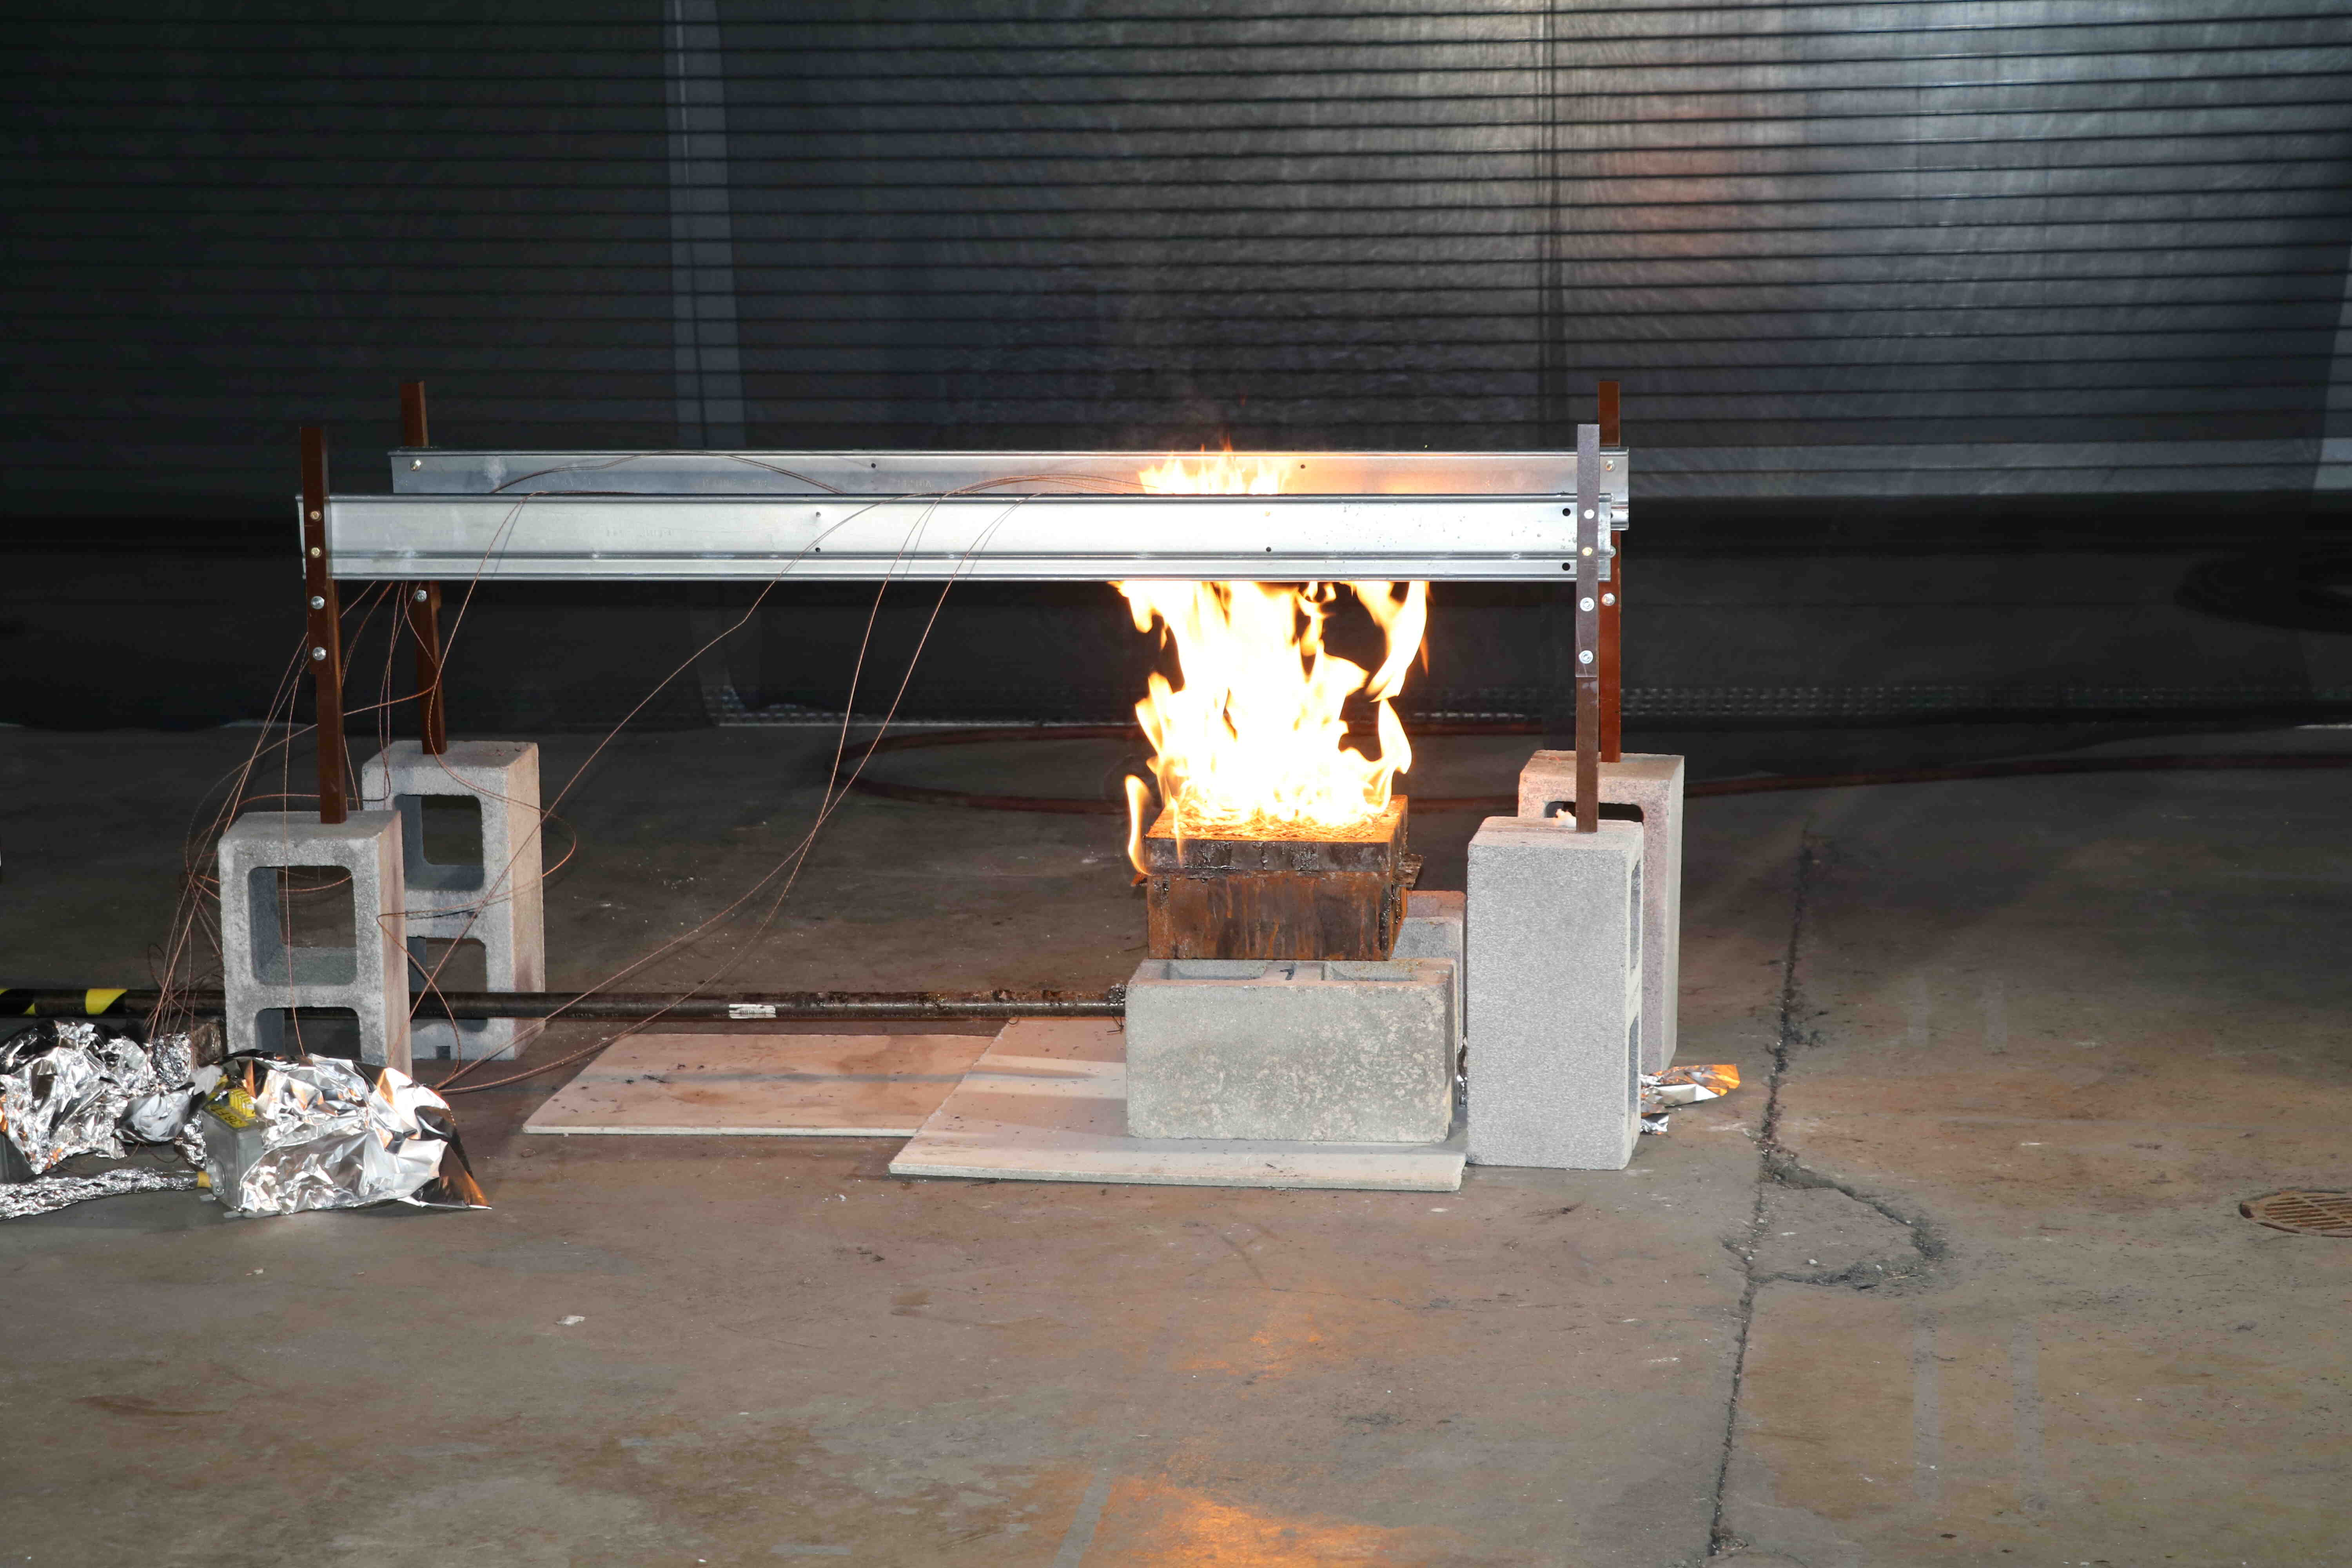
\includegraphics[height=2.75in]{../FIGURES/Test_36_side} \\
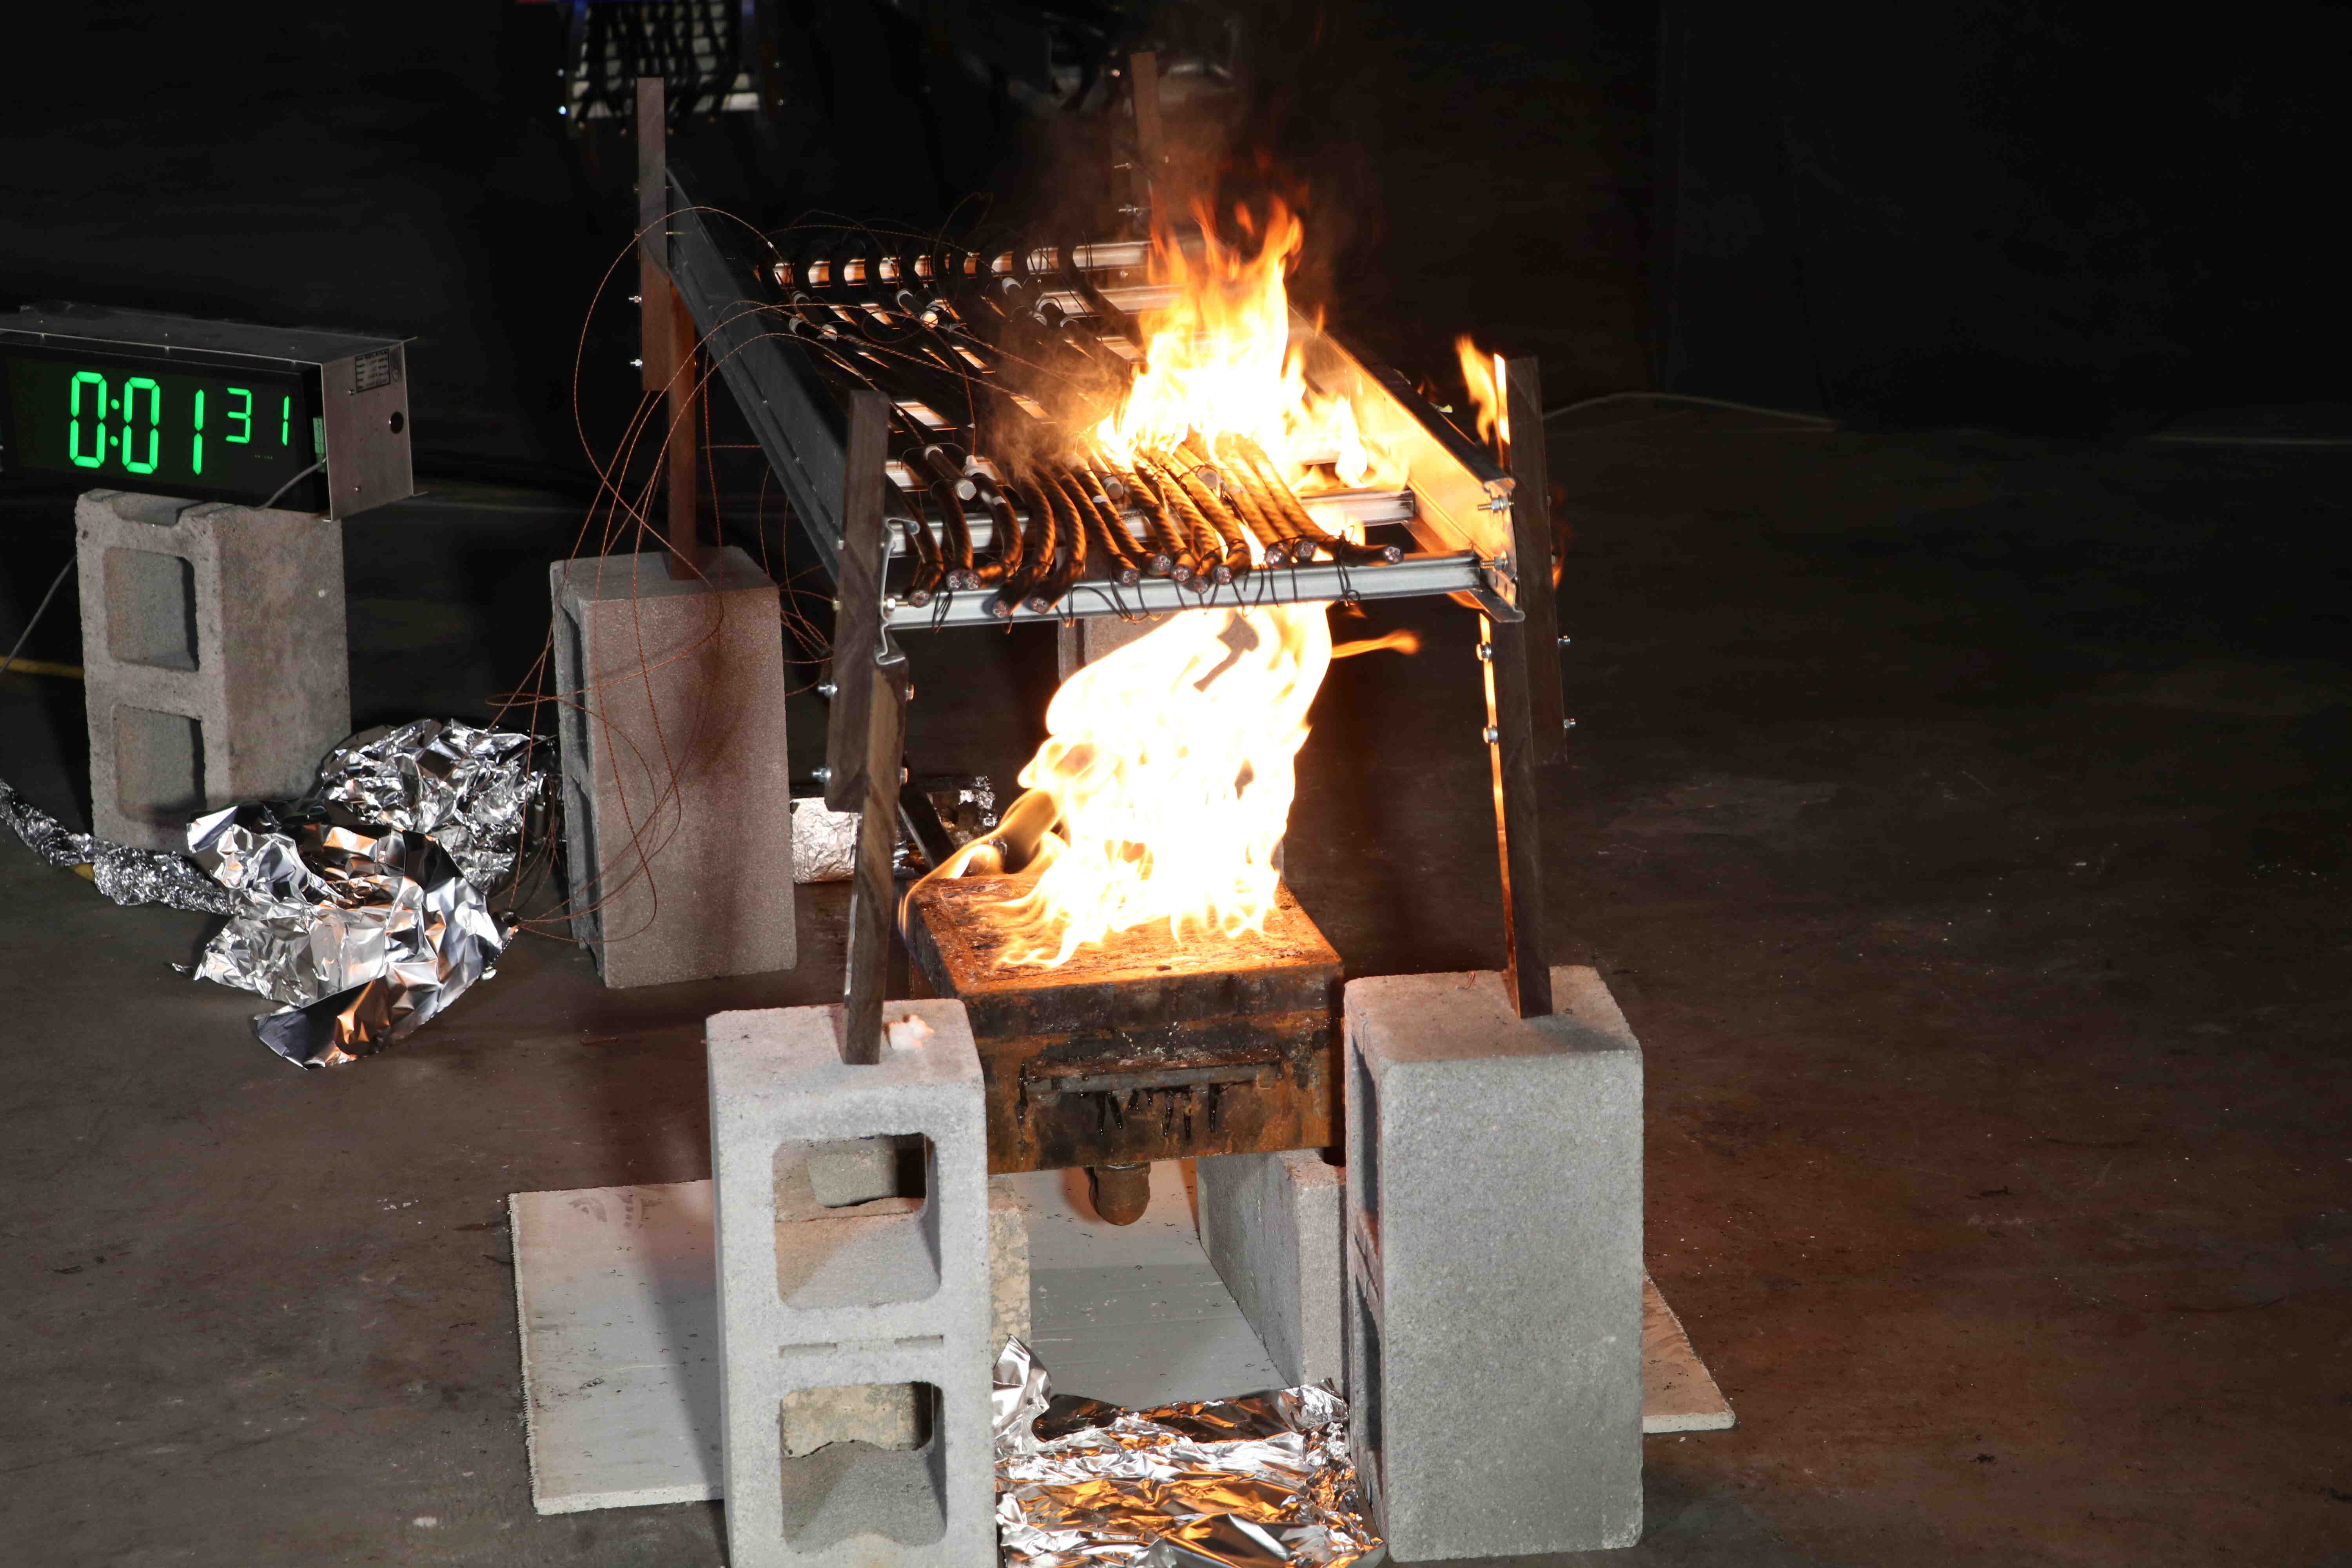
\includegraphics[height=2.75in]{../FIGURES/Test_36_1_min_31_s}
\caption[Photographs of Experiment~36]{Photographs of Experiment~36.}
\label{fig:Test_36_photos}
\end{figure}


\clearpage

\subsubsection{Experiment 37}

A 45~cm (18~in) wide tray containing 13 thermoplastic cables (\#900) was placed approximately 56~cm (22~in) above a nominally 30~cm square 40~kW natural gas burner. Thermocouples were inserted into three cables above the burner, and instrumented aluminum rods (``slugs'') were placed alongside the instrumented cables. The figures below show the heat release rate of the gas burner and the total heat release rate of the burner and cables, along with the internal temperatures of the cables and slugs. The cables ignited at approximately 5~min 30~s.

\begin{figure}[!h]
\begin{tabular*}{\textwidth}{l@{\extracolsep{\fill}}r}
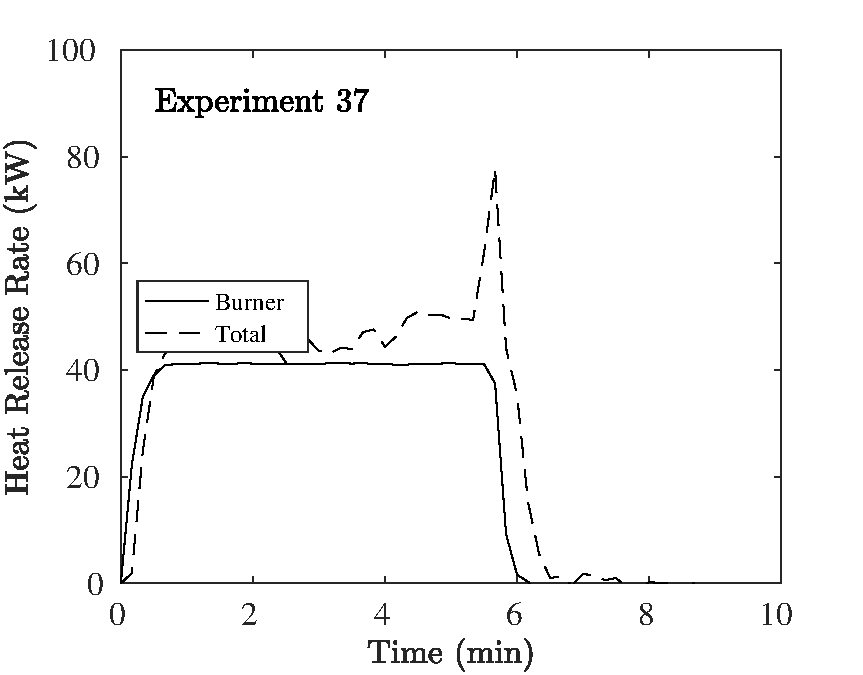
\includegraphics[height=2.65in]{../SCRIPT_FIGURES/Test_37_Plot_1} &
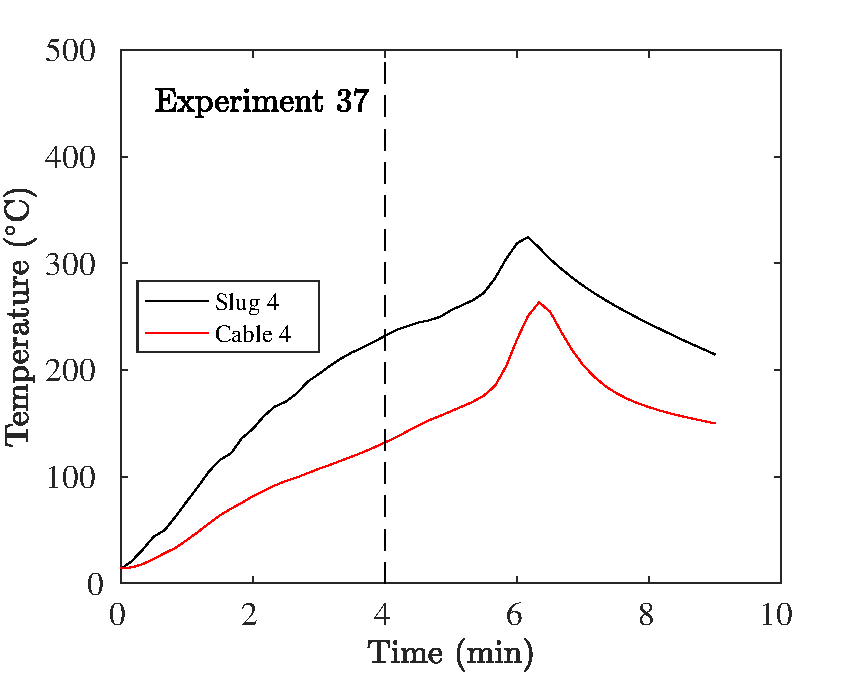
\includegraphics[height=2.65in]{../SCRIPT_FIGURES/Test_37_Plot_2} \\
\includegraphics[height=2.65in]{../SCRIPT_FIGURES/Test_37_Plot_3} &
\includegraphics[height=2.65in]{../SCRIPT_FIGURES/Test_37_Plot_4}
\end{tabular*}
\caption[HRR and temperatures of Experiment 37]{Heat release rate (upper left) and internal cable and slug temperatures above a 40~kW burner. The vertical dashed line indicates cable ignition.}
\label{fig:Test_37}
\end{figure}

\begin{figure}[p]
\centering
\includegraphics[height=2.75in]{../FIGURES/Test_37_side} \\
\includegraphics[height=2.75in]{../FIGURES/Test_37_1_min_36_s} \\
\includegraphics[height=2.75in]{../FIGURES/Test_37_ignition}
\caption[Photographs of Experiment~37]{Photographs of Experiment~37.}
\label{fig:Test_37_photos}
\end{figure}


\clearpage

\subsubsection{Experiment 38}

A 45~cm (18~in) wide tray containing 12 thermoset cables was placed approximately 56~cm (22~in) above a nominally 30~cm square 40~kW natural gas burner. Thermocouples were inserted into three cables above the burner, and instrumented aluminum rods (``slugs'') were placed alongside the instrumented cables. The figures below show the heat release rate of the gas burner and the total heat release rate of the burner and cables, along with the internal temperatures of the cables and slugs. The cables did not ignite.

\begin{figure}[!h]
\begin{tabular*}{\textwidth}{l@{\extracolsep{\fill}}r}
\includegraphics[height=2.65in]{../SCRIPT_FIGURES/Test_38_Plot_1} &
\includegraphics[height=2.65in]{../SCRIPT_FIGURES/Test_38_Plot_2} \\
\includegraphics[height=2.65in]{../SCRIPT_FIGURES/Test_38_Plot_3} &
\includegraphics[height=2.65in]{../SCRIPT_FIGURES/Test_38_Plot_4}
\end{tabular*}
\caption[HRR and temperatures of Experiment 38]{Heat release rate (upper left) and internal cable and slug temperatures above a 40~kW burner.}
\label{fig:Test_38}
\end{figure}

\begin{figure}[p]
\centering
\includegraphics[height=2.75in]{../FIGURES/Test_38_setup} \\
\includegraphics[height=2.75in]{../FIGURES/Test_38_29_min_29_s} \\
\includegraphics[height=2.75in]{../FIGURES/Test_38_damage}
\caption[Photographs of Experiment~38]{Photographs of Experiment~38.}
\label{fig:Test_38_photos}
\end{figure}


\clearpage

\subsubsection{Experiment 39}

A 45~cm (18~in) wide tray containing 12 thermoset cables was placed approximately 36~cm (14~in) above a nominally 30~cm square 40~kW natural gas burner. Thermocouples were inserted into three cables above the burner, and instrumented aluminum rods (``slugs'') were placed alongside the instrumented cables. The figures below show the heat release rate of the gas burner and the total heat release rate of the burner and cables, along with the internal temperatures of the cables and slugs. The cables ignited at approximately 1~min.

\begin{figure}[!h]
\begin{tabular*}{\textwidth}{l@{\extracolsep{\fill}}r}
\includegraphics[height=2.65in]{../SCRIPT_FIGURES/Test_39_Plot_1} &
\includegraphics[height=2.65in]{../SCRIPT_FIGURES/Test_39_Plot_2} \\
\includegraphics[height=2.65in]{../SCRIPT_FIGURES/Test_39_Plot_3} &
\includegraphics[height=2.65in]{../SCRIPT_FIGURES/Test_39_Plot_4}
\end{tabular*}
\caption[HRR and temperatures of Experiment 39]{Heat release rate (upper left) and internal cable and slug temperatures above a 40~kW burner. The vertical dashed line indicates cable ignition.}
\label{fig:Test_39}
\end{figure}

\begin{figure}[p]
\centering
\includegraphics[height=2.75in]{../FIGURES/Test_39_side} \\
\includegraphics[height=2.75in]{../FIGURES/Test_39_1_min_36_s} \\
\includegraphics[height=2.75in]{../FIGURES/Test_39_3_min_11_s}
\caption[Photographs of Experiment~39]{Photographs of Experiment~39.}
\label{fig:Test_39_photos}
\end{figure}


\clearpage

\subsubsection{Experiment 45}

A 45~cm (18~in) wide tray containing 34 thermoset cables was placed approximately 36~cm (14~in) above a nominally 30~cm square 40~kW natural gas burner. Thermocouples were inserted into two cables above the burner, and instrumented aluminum rods (``slugs'') were placed alongside the instrumented cables. The figures below show the heat release rate of the gas burner and the total heat release rate of the burner and cables, along with the internal temperatures of the cables and slugs. A small flame appeared in one location above the layer of cables at about 50~min, but the flame did not spread or lead to a wider, sustained ignition. Even though the cables did not fully ignite after an exposure of 1~h, but there was extensive damage and exposure of the copper wires.

\begin{figure}[!h]
\begin{tabular*}{\textwidth}{l@{\extracolsep{\fill}}r}
\includegraphics[height=2.65in]{../SCRIPT_FIGURES/Test_45_Plot_1} &
\includegraphics[height=2.65in]{../SCRIPT_FIGURES/Test_45_Plot_2} \\
\multicolumn{2}{c}{\includegraphics[height=2.65in]{../SCRIPT_FIGURES/Test_45_Plot_3}}
\end{tabular*}
\caption[HRR and temperatures of Experiment 45]{Heat release rate (upper left) and internal cable and slug temperatures above a 40~kW burner. The vertical dashed line indicates cable ignition.}
\label{fig:Test_45}
\end{figure}

\begin{figure}[p]
\centering
\includegraphics[height=2.75in]{../FIGURES/Test_45_setup} \\
\includegraphics[height=2.75in]{../FIGURES/Test_45_42_min_46_s} \\
\includegraphics[height=2.75in]{../FIGURES/Test_45_damage}
\caption[Photographs of Experiment~45]{Photographs of Experiment~45.}
\label{fig:Test_45_photos}
\end{figure}


\clearpage

\subsubsection{Experiment 46}

This experiment is similar to Exp.~45 except that every seventh cable has been removed, leaving 30 rather than 34 across the width of the tray. The figures below show the heat release rate of the gas burner and the total heat release rate of the burner and cables, along with the internal temperatures of the cables and slugs. The cables ignite at approximately 12~min.

\begin{figure}[!h]
\begin{tabular*}{\textwidth}{l@{\extracolsep{\fill}}r}
\includegraphics[height=2.65in]{../SCRIPT_FIGURES/Test_46_Plot_1} &
\includegraphics[height=2.65in]{../SCRIPT_FIGURES/Test_46_Plot_2} \\
\multicolumn{2}{c}{\includegraphics[height=2.65in]{../SCRIPT_FIGURES/Test_46_Plot_3}}
\end{tabular*}
\caption[HRR and temperatures of Experiment 46]{Heat release rate (upper left) and internal cable and slug temperatures above a 40~kW burner. The vertical dashed line indicates cable ignition.}
\label{fig:Test_46}
\end{figure}

\begin{figure}[p]
\centering
\includegraphics[height=2.75in]{../FIGURES/Test_46_setup} \\
\includegraphics[height=2.75in]{../FIGURES/Test_46_ignition} \\
\includegraphics[height=2.75in]{../FIGURES/Test_46_burning}
\caption[Photographs of Experiment~46]{Photographs of Experiment~46.}
\label{fig:Test_46_photos}
\end{figure}


\clearpage

\subsubsection{Experiment 47}

A 45~cm (18~in) wide tray containing 30 thermoplastic cables (\#900) was placed approximately 36~cm (14~in) above a nominally 30~cm square 40~kW natural gas burner. Thermocouples were inserted into two cables above the burner, and instrumented aluminum rods (``slugs'') were placed alongside the instrumented cables. The figures below show the heat release rate of the gas burner and the total heat release rate of the burner and cables, along with the internal temperatures of the cables and slugs. The cables ignited in less than 1~min.

\begin{figure}[!h]
\begin{tabular*}{\textwidth}{l@{\extracolsep{\fill}}r}
\includegraphics[height=2.65in]{../SCRIPT_FIGURES/Test_47_Plot_1} &
\includegraphics[height=2.65in]{../SCRIPT_FIGURES/Test_47_Plot_2} \\
\multicolumn{2}{c}{\includegraphics[height=2.65in]{../SCRIPT_FIGURES/Test_47_Plot_3}}
\end{tabular*}
\caption[HRR and temperatures of Experiment 47]{Heat release rate (upper left) and internal cable and slug temperatures above a 40~kW burner. The vertical dashed line indicates cable ignition.}
\label{fig:Test_47}
\end{figure}

\begin{figure}[p]
\centering
\includegraphics[height=2.75in]{../FIGURES/Test_47_setup} \\
\includegraphics[height=2.75in]{../FIGURES/Test_47_ignition} \\
\includegraphics[height=2.75in]{../FIGURES/Test_47_burning}
\caption[Photographs of Experiment~47]{Photographs of Experiment~47.}
\label{fig:Test_47_photos}
\end{figure}


\clearpage

\subsubsection{Experiment 48}

Experiment 48 was the same as Exp.~47 except that the tray was increased to 56~cm (22~in) above the burner. The figures below show the heat release rate of the gas burner and the total heat release rate of the burner and cables, along with the internal temperatures of the cables and slugs. The cables ignited at approximately 3~min.

\begin{figure}[!h]
\begin{tabular*}{\textwidth}{l@{\extracolsep{\fill}}r}
\includegraphics[height=2.65in]{../SCRIPT_FIGURES/Test_48_Plot_1} &
\includegraphics[height=2.65in]{../SCRIPT_FIGURES/Test_48_Plot_2} \\
\multicolumn{2}{c}{\includegraphics[height=2.65in]{../SCRIPT_FIGURES/Test_48_Plot_3}}
\end{tabular*}
\caption[HRR and temperatures of Experiment 48]{Heat release rate (upper left) and internal cable and slug temperatures above a 40~kW burner. The vertical dashed line indicates cable ignition.}
\label{fig:Test_48}
\end{figure}

\begin{figure}[p]
\centering
\includegraphics[height=2.75in]{../FIGURES/Test_48_1_min_3_s} \\
\includegraphics[height=2.75in]{../FIGURES/Test_48_3_min_11_s} \\
\includegraphics[height=2.75in]{../FIGURES/Test_48_3_min_28_s}
\caption[Photographs of Experiment~48]{Photographs of Experiment~48.}
\label{fig:Test_48_photos}
\end{figure}


\clearpage

\subsubsection{Summary}

\begin{table}[ht]
\begin{center}
\caption[Results of cable tray ignition experiments]{Ignition time of cables set above a 40~kW natural gas burner.}
\label{matrix}
\begin{tabular}{|c|c|c|c|c|}
\hline
Exp.   &          & Cable             & Cable         & Ignition         \\
No.    & Make     & Packing           & Height        & Time             \\
       &          &                   & (cm)          & (min:s)          \\ \hline
36     & TP       & Loose             & 36            & 1:30             \\ \hline
37     & TP       & Loose             & 56            & 4:00             \\ \hline
38     & TS       & Loose             & 56            & ---              \\ \hline
39     & TS       & Loose             & 36            & 1:30             \\ \hline
45     & TS       & Tight             & 36            & 50:00            \\ \hline
46     & TS       & Tight             & 36            & 12:00            \\ \hline
47     & TP       & Tight             & 36            & 1:00             \\ \hline
36     & TP       & Tight             & 56            & 3:00             \\ \hline

\end{tabular}
\end{center}
\end{table}



\clearpage

\subsection{Measuring the Gas Temperature above a Burning Enclosure}

Following the HRR measurements in Experiments 40 and 41, the same Westinghouse enclosure was used in experiments aimed at measuring the fire plume temperature outside of a near-ceiling vertical vent. These were difficult measurements to perform because it is difficult to predict the trajectory of the plume centerline. Nevertheless, it can be seen in Experiments~42 through 45 that temperatures above a vertical vent can reach values of 400~$^\circ$C to 500~$^\circ$C (750~$^\circ$F to 930~$^\circ$F), high enough to ignite cables given enough time, a subject which is the focus of Experiments~49 through 64.



\clearpage


\subsubsection{Experiment 42}

A 30~cm (12~in) square natural gas burner was positioned in the mostly empty space at the rear of the breaker enclosure used in previous experiments. The heat release rate of the burner was ramped up to 200~kW following an approximate t-squared profile. Six sheathed thermocouples were positioned above the upper rear vent in an attempt to measure the plume temperature. The plume did follow the expected pattern; thus, this experiment is of little value.

The figures below show the heat release rate of the gas burner and the total heat release rate of the burner and cables, along with the temperatures measured by the sheathed thermocouples above the enclosure.

\begin{figure}[!h]
\begin{tabular*}{\textwidth}{l@{\extracolsep{\fill}}r}
\includegraphics[height=2.65in]{../SCRIPT_FIGURES/Test_42_Plot_1} &
\includegraphics[height=2.65in]{../SCRIPT_FIGURES/Test_42_Plot_2}
\end{tabular*}
\caption[HRR and temperatures of Experiment 42]{Heat release rate (upper left) and various temperatures inside and above a burning breaker enclosure.}
\label{fig:Test_42}
\end{figure}

\begin{figure}[p]
\centering
\includegraphics[height=2.75in]{../FIGURES/Test_42_start} \\
\includegraphics[height=2.75in]{../FIGURES/Test_42_rear} \\
\includegraphics[height=2.75in]{../FIGURES/Test_42_side}
\caption[Photographs of Experiment~42]{Photographs of Experiment~42.}
\label{fig:Test_42_photos}
\end{figure}


\clearpage

\subsubsection{Experiment 43}

A 30~cm (12~in) square natural gas burner was positioned in the mostly empty space at the rear of the breaker enclosure used in previous experiments. The heat release rate of the burner was ramped up to 300~kW following an approximate t-squared profile. Six aluminum rods (``slugs'') and six sheathed thermocouples were positioned above the upper rear vent in an attempt to measure the plume temperature. Two of each instrument were positioned approximately 15~cm (6~in), 30~cm (12~in), and 60~cm (24~in) above the top of the enclosure, roughly flush with the rear door.

The figures below show the heat release rate of the gas burner and the total heat release rate of the burner and cables, along with the temperatures measured by the sheathed thermocouples above the enclosure.

\begin{figure}[!h]
\begin{tabular*}{\textwidth}{l@{\extracolsep{\fill}}r}
\includegraphics[height=2.65in]{../SCRIPT_FIGURES/Test_43_Plot_1} &
\includegraphics[height=2.65in]{../SCRIPT_FIGURES/Test_43_Plot_2} \\
\multicolumn{2}{c}{\includegraphics[height=2.65in]{../SCRIPT_FIGURES/Test_43_Plot_3}}
\end{tabular*}
\caption[HRR and temperatures of Experiment 43]{Heat release rate (upper left) and various temperatures inside and above a burning breaker enclosure.}
\label{fig:Test_43}
\end{figure}

\begin{figure}[p]
\centering
\includegraphics[height=2.75in]{../FIGURES/Test_43_setup} \\
\includegraphics[height=2.75in]{../FIGURES/Test_43_9_min_12_s} \\
\includegraphics[height=2.75in]{../FIGURES/Test_43_side}
\caption[Photographs of Experiment~43]{Photographs of Experiment~43.}
\label{fig:Test_43_photos}
\end{figure}


\clearpage

\subsubsection{Experiment 44}

Experiment~44 was similar to Experiment~43 except that more vents at the rear of the enclosure were closed.

The figures below show the heat release rate of the gas burner and the total heat release rate of the burner and cables, along with the temperatures measured by the sheathed thermocouples above the enclosure.

\begin{figure}[!h]
\begin{tabular*}{\textwidth}{l@{\extracolsep{\fill}}r}
\includegraphics[height=2.65in]{../SCRIPT_FIGURES/Test_44_Plot_1} &
\includegraphics[height=2.65in]{../SCRIPT_FIGURES/Test_44_Plot_2} \\
\multicolumn{2}{c}{\includegraphics[height=2.65in]{../SCRIPT_FIGURES/Test_44_Plot_3}}
\end{tabular*}
\caption[HRR and temperatures of Experiment 44]{Heat release rate (upper left) and various temperatures inside and above a burning breaker enclosure.}
\label{fig:Test_44}
\end{figure}

\begin{figure}[p]
\centering
\includegraphics[height=2.75in]{../FIGURES/Test_44_start} \\
\includegraphics[height=2.75in]{../FIGURES/Test_44_15_min_19_s} \\
\includegraphics[height=2.75in]{../FIGURES/Test_44_side}
\caption[Photographs of Experiment~44]{Photographs of Experiment~44.}
\label{fig:Test_44_photos}
\end{figure}


\clearpage


\subsection{Measuring Cable Temperatures above an Enclosure Fire}

Experiments 49 through 64, conducted in March 2024, made use of two empty electrical enclosures used in a previous set of experiments~\cite{OLIVE-FIRE}. Drawings are shown in Fig.~\ref{fig:enclosure_drawings}. One or two 30~cm (12~in) wide cable trays were positioned on top of the enclosures. The trays contained (usually) ten thermoplastic or thermoset cables, some of which were instrumented with a thermocouple embedded in its center amongst the conductors. Aluminum rods (``slugs'') were also placed on top of the cables in the vicinity of the embedded thermocouples. While the slug and cable temperatures are not an exact match, the slugs are useful as comparisons with future modeling studies.
\begin{figure}[!ht]
\hspace*{-0.75in}\includegraphics[height=4.75in]{../FIGURES/Cabinet_3}
\hspace*{-1.25in}\includegraphics[height=4.75in]{../FIGURES/Cabinet_1}
\caption[Drawings of Enclosures \#2 and \#3]{Drawings of Enclosure~\#3 (left) and \#2 (right).}
\label{fig:enclosure_drawings}
\end{figure}
Sheathed thermocouples were also positioned above the trays to measure the plume (gas) temperature, but these measurements are of little value because they rarely capture the peak plume temperature or the actual exposing temperature of the cables. The reason is that the plume centerline does not follow a vertical path, but rather jets out of the vent and then turns back towards the enclosure face. The path changes as the fire grows. Initially the fairly weak plume is drawn inwards towards the top of the enclosure, but then extends outwards as the fire grows and the plume temperature increases.

The same 30~cm (12~in) natural gas burner used in previous experiments was positioned in the center of Enclosure~\#3, approximately 1.5~m (60~in) below the ceiling, or below the left vent in Enclosure~\#2, approximately 56~cm (22~in) below the ceiling. The heat release rate profile was varied, but in all cases it was designed to ignite the cables.


\clearpage


\subsubsection{Experiment 49}

Two 30~cm (12~in) wide cable trays were set 30~cm (12~in) above an enclosure measuring approximately 0.91~m (36~in) wide and 1.40~m (55~in) deep. Each tray overhung a louvered vent whose top edge was approximately 8~cm (3~in) below the top of the enclosure. The burner was positioned approximately 1.5~m (60~in) below the ceiling of the enclosure in the position shown in Fig.~\ref{Exp_49_diagram}. The fire was set to approximately 100~kW for 10~minutes and then increased to 200~kW for an additional 5~min. No flames were observed exiting the upper vent, and the natural gas flow was increased again to sustain a 300~kW and then 400~kW fire. However, due to ventilation limitations, the actual heat release rate of the fire did not surpass 200~kW, and the natural gas flow was decreased to that level. Flames were not observed exiting the vent at any time during the experiment and the target temperatures did not surpass 200~$^\circ$C.

\setlength{\unitlength}{0.03in}
\begin{figure}[!h]
\centering
\begin{picture}(70,40)(0,0)
\put(0,0){\framebox(55,36){ }}
\put(33,11){\dashbox(14,14){ }}
\thicklines
\multiput(-15,20)(0,12){2}{\line(1,0){108}}
\multiput(-9,20)(9,0){12}{\line(0,1){12}}
\multiput(-15,4)(0,12){2}{\line(1,0){108}}
\multiput(-9,4)(9,0){12}{\line(0,1){12}}
\put(56, 7){\tiny 4/5}
\put(56,11){\tiny 39/40}
\put(65, 7){\tiny 2/3}
\put(65,11){\tiny 36/38}
\put(74, 7){\tiny 1}
\put(74,11){\tiny 37}
\put(56,23){\tiny 9/10}
\put(56,27){\tiny 23/24}
\put(65,23){\tiny 7/8}
\put(65,27){\tiny 21/22}
\put(74,23){\tiny 6}
\put(74,27){\tiny 25}
\put(95,17){Front}
\end{picture}
\caption[Plan view of Experiment 49]{Plan view of the Enclosure~\#3 with cable trays set on top. The dashed box indicates the location of the burner within the enclosure. The numbers refer to either the aluminum slugs (1-20) or instrumented cables (21-40). The tray in the lower part of the figure held 10 thermoset cables; the other held 10 thermoplastic cables.}
\label{Exp_49_diagram}
\end{figure}

\begin{figure}[!h]
\begin{tabular*}{\textwidth}{l@{\extracolsep{\fill}}r}
\includegraphics[height=2.65in]{../SCRIPT_FIGURES/Test_49_Plot_1} &
\includegraphics[height=2.65in]{../SCRIPT_FIGURES/Test_49_Plot_2}
\end{tabular*}
\caption[HRR and temperatures of Experiment 49]{Heat release rate (left) and peak target temperatures (right) for Exp.~49.}
\label{fig:Test_49}
\end{figure}

\begin{figure}[p]
\centering
\includegraphics[height=2.75in]{../FIGURES/Test_49_setup} \\
\includegraphics[height=2.75in]{../FIGURES/Test_49_cables} \\
\includegraphics[height=2.75in]{../FIGURES/Test_49_fire}
\caption[Photographs of Experiment~49]{Photographs of Experiment~49.}
\label{fig:Test_49_photos}
\end{figure}


\clearpage

\subsubsection{Experiment 50}

This experiment retained the same basic setup as Exp.~49 except that the louvered vent was removed leaving a 20~cm (8~in) tall vent across the width of the enclosure, 8~cm (3~in) below the top. In addition, the trays were shifted so that the leftmost cable and slug targets shown in Fig.~\ref{Exp_50_diagram} would fall within the smoke plume observed in Exp.~49. However, because the vent louvers were removed, the flames and plume were thrust further to the right, and no targets were directly impacted. As a result, this experiment did not yield a meaningful target temperature at the time of ignition.

\setlength{\unitlength}{0.03in}
\begin{figure}[!h]
\centering
\begin{picture}(70,40)(0,0)
\put(0,0){\framebox(55,36){ }}
\put(33,11){\dashbox(14,14){ }}
\thicklines
\multiput(-24,20)(0,12){2}{\line(1,0){108}}
\multiput(-18,20)(9,0){12}{\line(0,1){12}}
\multiput(-24,4)(0,12){2}{\line(1,0){108}}
\multiput(-18,4)(9,0){12}{\line(0,1){12}}
\put(47, 7){\tiny 4/5}
\put(47,11){\tiny 39/40}
\put(56, 7){\tiny 2/3}
\put(56,11){\tiny 36/38}
\put(65, 7){\tiny 1}
\put(65,11){\tiny 37}
\put(47,23){\tiny 9/10}
\put(47,27){\tiny 23/24}
\put(56,23){\tiny 7/8}
\put(56,27){\tiny 21/22}
\put(65,23){\tiny 6}
\put(65,27){\tiny 25}
\put(86,17){Front}
\end{picture}
\caption[Plan view of Experiment 50]{Plan view of the enclosure with cable trays set on top. The dashed box indicates the location of the burner within the enclosure. The numbers refer to either the aluminum slugs (1-20) or instrumented cables (21-40). The tray in the lower part of the figure held 10 thermoset cables; the other held 10 thermoplastic cables.}
\label{Exp_50_diagram}
\end{figure}

\begin{figure}[!h]
\begin{tabular*}{\textwidth}{l@{\extracolsep{\fill}}r}
\includegraphics[height=2.65in]{../SCRIPT_FIGURES/Test_50_Plot_1} &
\includegraphics[height=2.65in]{../SCRIPT_FIGURES/Test_50_Plot_2}
\end{tabular*}
\caption[HRR and temperatures of Experiment 50]{Heat release rate (left) and peak target temperatures (right) for Exp.~50.}
\label{fig:Test_50}
\end{figure}

\begin{figure}[p]
\centering
\includegraphics[height=2.75in]{../FIGURES/Test_50_cables} \\
\includegraphics[height=2.75in]{../FIGURES/Test_50_side} \\
\includegraphics[height=2.75in]{../FIGURES/Test_50_20_min_58_s}
\caption[Photographs of Experiment~50]{Photographs of Experiment~50.}
\label{fig:Test_50_photos}
\end{figure}


\clearpage

\subsubsection{Experiment 51}

Two cable trays were set 30~cm (12~in) above Enclosure~\#2 which measured approximately 1.68~m (66~in) wide and 1.52~m (60~in) deep. Each tray overhung a grilled vent whose top edge was approximately 10~cm (4~in) below the top of the enclosure. The burner was positioned approximately 56~cm (22~in) below the ceiling of the enclosure in the position shown in Fig.~\ref{Exp_51_diagram}. The thermoset cables in the tray directly above the left upper vent ignited after approximately 18~min. The thermoplastic cables in the second tray did not ignite.

\setlength{\unitlength}{0.03in}
\begin{figure}[!h]
\centering
\begin{picture}(70,70)(0,0)
\put(0,0){\framebox(60,66){ }}
\put(38,9){\dashbox(14,14){ }}
\thicklines
\multiput(-20,44)(0,12){2}{\line(1,0){108}}
\multiput(-14,44)(9,0){12}{\line(0,1){12}}
\multiput(-20,10)(0,12){2}{\line(1,0){108}}
\multiput(-14,10)(9,0){12}{\line(0,1){12}}
\put(43,13){\tiny 6}
\put(43,17){\tiny 23}
\put(52,13){\tiny 7}
\put(52,17){\tiny 22}
\put(61,13){\tiny 8}
\put(61,17){\tiny 21}
\put(70,13){\tiny 9}
\put(70,17){\tiny 40}
\put(79,13){\tiny 10}
\put(79,17){\tiny 24}
\put(43,47){\tiny 3}
\put(43,51){\tiny 25}
\put(52,47){\tiny 2}
\put(52,51){\tiny 37}
\put(61,47){\tiny 1}
\put(61,51){\tiny 38}
\put(70,47){\tiny 5}
\put(70,51){\tiny 36}
\put(79,47){\tiny 4}
\put(79,51){\tiny 39}
\put(64,31){Front}
\end{picture}
\caption[Plan view of Experiment 51]{Plan view of the enclosure with cable trays set on top. The dashed box indicates the location of the burner within the enclosure. The numbers refer to either the aluminum slugs (1-20) or instrumented cables (21-40). The tray directly above the burner held 10 thermoset cables; the other held 10 thermoplastic cables.}
\label{Exp_51_diagram}
\end{figure}

\begin{figure}[!h]
\begin{tabular*}{\textwidth}{l@{\extracolsep{\fill}}r}
\includegraphics[height=2.65in]{../SCRIPT_FIGURES/Test_51_Plot_1} &
\includegraphics[height=2.65in]{../SCRIPT_FIGURES/Test_51_Plot_3}
\end{tabular*}
\caption[HRR and temperatures of Exp.~51]{Heat release rate and target temperatures for Exp.~51. The ignition time of the thermoset cables directly above the burner is indicated by the vertical dashed line. The cables in the other tray did not ignite.}
\label{fig:Test_51}
\end{figure}

\begin{figure}[p]
\centering
\includegraphics[height=2.75in]{../FIGURES/Test_51_setup} \\
\includegraphics[height=2.75in]{../FIGURES/Test_51_ignition} \\
\includegraphics[height=2.75in]{../FIGURES/Test_51_scar}
\caption[Photographs of Experiment~51]{Photographs of Experiment~51.}
\label{fig:Test_51_photos}
\end{figure}


\clearpage

\subsubsection{Experiment 52}

This experiment is similar to Exp.~51 except that a single cable tray of thermoplastic cables was set approximately 30~cm (12~in) above the enclosure, directly in line with the fire plume exiting the left upper vent. The cables ignited after approximately 11~min.


\setlength{\unitlength}{0.03in}
\begin{figure}[!h]
\centering
\begin{picture}(70,70)(0,0)
\put(0,0){\framebox(60,66){ }}
\put(38,9){\dashbox(14,14){ }}
\thicklines
\multiput(-20,10)(0,12){2}{\line(1,0){108}}
\multiput(-14,10)(9,0){12}{\line(0,1){12}}
\put(43,13){\tiny 3}
\put(43,17){\tiny 25}
\put(52,13){\tiny 2}
\put(52,17){\tiny 37}
\put(61,13){\tiny 1}
\put(61,17){\tiny 38}
\put(70,13){\tiny 5}
\put(70,17){\tiny 36}
\put(79,13){\tiny 4}
\put(79,17){\tiny 39}
\put(64,31){Front}
\end{picture}
\caption[Plan view of Exp.~52]{Plan view of the enclosure with cable trays set on top. The dashed box indicates the location of the burner within the enclosure. The numbers refer to either the aluminum slugs (1-20) or instrumented cables (21-40). The tray held 10 thermoset cables.}
\label{Exp_52_diagram}
\end{figure}


\begin{figure}[!h]
\begin{tabular*}{\textwidth}{l@{\extracolsep{\fill}}r}
\includegraphics[height=2.65in]{../SCRIPT_FIGURES/Test_52_Plot_1} &
\includegraphics[height=2.65in]{../SCRIPT_FIGURES/Test_52_Plot_3}
\end{tabular*}
\caption[HRR and temperatures of Experiment 52]{Heat release rate (left) and peak target temperatures (right) for Exp.~52.}
\label{fig:Test_52}
\end{figure}

\begin{figure}[p]
\centering
\includegraphics[height=2.75in]{../FIGURES/Test_52_3_min_15_s} \\
\includegraphics[height=2.75in]{../FIGURES/Test_52_10_min_17_s} \\
\includegraphics[height=2.75in]{../FIGURES/Test_52_11_min_50_s}
\caption[Photographs of Experiment~52]{Photographs of Experiment~52.}
\label{fig:Test_52_photos}
\end{figure}


\clearpage

\subsubsection{Experiment 53}

This experiment is similar to Exp.~52 except that a different heat release rate ramp was implemented to better mimic a so-called ``t-squared'' fire, where the HRR ramps up to 200~kW in 12~min following a quadratic time function. The thermoplastic cables ignited after approximately 11~min.


\setlength{\unitlength}{0.03in}
\begin{figure}[!h]
\centering
\begin{picture}(70,70)(0,0)
\put(0,0){\framebox(60,66){ }}
\put(38,9){\dashbox(14,14){ }}
\thicklines
\multiput(-20,10)(0,12){2}{\line(1,0){108}}
\multiput(-14,10)(9,0){12}{\line(0,1){12}}
\put(43,13){\tiny 15}
\put(43,17){\tiny 35}
\put(52,13){\tiny 14}
\put(52,17){\tiny 34}
\put(61,13){\tiny 13}
\put(61,17){\tiny 33}
\put(70,13){\tiny 12}
\put(70,17){\tiny 32}
\put(79,13){\tiny 11}
\put(79,17){\tiny 31}
\put(64,31){Front}
\end{picture}
\caption[Plan view of Exp.~53]{Plan view of the enclosure with cable trays set on top. The dashed box indicates the location of the burner within the enclosure. The numbers refer to either the aluminum slugs (1-20) or instrumented cables (21-40). The tray held 10 thermoplastic cables.}
\label{Exp_53_diagram}
\end{figure}

\begin{figure}[!h]
\begin{tabular*}{\textwidth}{l@{\extracolsep{\fill}}r}
\includegraphics[height=2.65in]{../SCRIPT_FIGURES/Test_53_Plot_1} &
\includegraphics[height=2.65in]{../SCRIPT_FIGURES/Test_53_Plot_3}
\end{tabular*}
\caption[HRR and temperatures of Experiment 53]{Heat release rate (left) and peak target temperatures (right) for Exp.~53.}
\label{fig:Test_53}
\end{figure}

\begin{figure}[p]
\centering
\includegraphics[height=2.75in]{../FIGURES/Test_53_5_min_24_s} \\
\includegraphics[height=2.75in]{../FIGURES/Test_53_11_min_45_s} \\
\includegraphics[height=2.75in]{../FIGURES/Test_53_ignition}
\caption[Photographs of Experiment~53]{Photographs of Experiment~53.}
\label{fig:Test_53_photos}
\end{figure}


\clearpage

\subsubsection{Experiment 54}

This experiment is the same as Exp.~53 except that 10 thermoset cables were laid into the tray. They ignited after approximately 20~min.


\setlength{\unitlength}{0.03in}
\begin{figure}[!h]
\centering
\begin{picture}(70,70)(0,0)
\put(0,0){\framebox(60,66){ }}
\put(38,9){\dashbox(14,14){ }}
\thicklines
\multiput(-20,10)(0,12){2}{\line(1,0){108}}
\multiput(-14,10)(9,0){12}{\line(0,1){12}}
\put(43,13){\tiny 10}
\put(43,17){\tiny 25}
\put(52,13){\tiny  9}
\put(52,17){\tiny 24}
\put(61,13){\tiny  8}
\put(61,17){\tiny 23}
\put(70,13){\tiny  7}
\put(70,17){\tiny 22}
\put(79,13){\tiny  6}
\put(79,17){\tiny 21}
\put(64,31){Front}
\end{picture}
\caption[Plan view of Exp.~54]{Plan view of the enclosure with cable trays set on top. The dashed box indicates the location of the burner within the enclosure. The numbers refer to either the aluminum slugs (1-20) or instrumented cables (21-40). The tray held 10 thermoset cables.}
\label{Exp_54_diagram}
\end{figure}

\begin{figure}[!h]
\begin{tabular*}{\textwidth}{l@{\extracolsep{\fill}}r}
\includegraphics[height=2.65in]{../SCRIPT_FIGURES/Test_54_Plot_1} &
\includegraphics[height=2.65in]{../SCRIPT_FIGURES/Test_54_Plot_3}
\end{tabular*}
\caption[HRR and temperatures of Experiment 54]{Heat release rate (left) and peak target temperatures (right) for Exp.~54.}
\label{fig:Test_54}
\end{figure}

\begin{figure}[p]
\centering
\includegraphics[height=2.75in]{../FIGURES/Test_54_cables} \\
\includegraphics[height=2.75in]{../FIGURES/Test_54_15_min_20_s} \\
\includegraphics[height=2.75in]{../FIGURES/Test_54_22_min_31_s}
\caption[Photographs of Experiment~54]{Photographs of Experiment~54.}
\label{fig:Test_54_photos}
\end{figure}


\clearpage

\subsubsection{Experiment 55}

This is a replicate of Exp.~53, but with the cable and slug targets moved closer together to provide additional measurements of the plume centerline temperature. The thermoplastic cables ignited after approximately 12~min.

\setlength{\unitlength}{0.03in}
\begin{figure}[!h]
\centering
\begin{picture}(70,70)(0,0)
\put(0,0){\framebox(60,66){ }}
\put(38,9){\dashbox(14,14){ }}
\thicklines
\multiput(-20,10)(0,12){2}{\line(1,0){108}}
\multiput(-14,10)(9,0){12}{\line(0,1){12}}
\put(50,13){\tiny 19/20}
\put(50,17){\tiny 29/30}
\put(59,13){\tiny 17/18}
\put(59,17){\tiny 27/28}
\put(70,13){\tiny 16}
\put(70,17){\tiny 26}
\put(64,31){Front}
\end{picture}
\caption[Plan view of Exp.~55]{Plan view of the enclosure with cable trays set on top. The dashed box indicates the location of the burner within the enclosure. The numbers refer to either the aluminum slugs (1-20) or instrumented cables (21-40). The tray held 10 thermoplastic cables.}
\label{Exp_55_diagram}
\end{figure}

\begin{figure}[!h]
\begin{tabular*}{\textwidth}{l@{\extracolsep{\fill}}r}
\includegraphics[height=2.65in]{../SCRIPT_FIGURES/Test_55_Plot_1} &
\includegraphics[height=2.65in]{../SCRIPT_FIGURES/Test_55_Plot_3}
\end{tabular*}
\caption[HRR and temperatures of Experiment 55]{Heat release rate (left) and peak target temperatures (right) for Exp.~55.}
\label{fig:Test_55}
\end{figure}

\begin{figure}[p]
\centering
\includegraphics[height=2.75in]{../FIGURES/Test_55_cables} \\
\includegraphics[height=2.75in]{../FIGURES/Test_55_14_min_54_s}
\caption[Photographs of Experiment~55]{Photographs of Experiment~55.}
\label{fig:Test_55_photos}
\end{figure}


\clearpage

\subsubsection{Experiment 56}

This is a replicate of Exp.~54, but with the cable and slug targets moved closer together to provide additional measurements of the plume centerline temperature. The thermoset cables ignited after approximately 22~min.

\setlength{\unitlength}{0.03in}
\begin{figure}[!h]
\centering
\begin{picture}(70,70)(0,0)
\put(0,0){\framebox(60,66){ }}
\put(38,9){\dashbox(14,14){ }}
\thicklines
\multiput(-20,10)(0,12){2}{\line(1,0){108}}
\multiput(-14,10)(9,0){12}{\line(0,1){12}}
\put(50,13){\tiny  9/11}
\put(50,17){\tiny 24/25}
\put(59,13){\tiny 7/8}
\put(59,17){\tiny 22/23}
\put(70,13){\tiny 6}
\put(70,17){\tiny 21}
\put(64,31){Front}
\end{picture}
\caption[Plan view of Exp.~56]{Plan view of the enclosure with cable trays set on top. The dashed box indicates the location of the burner within the enclosure. The numbers refer to either the aluminum slugs (1-20) or instrumented cables (21-40). The tray held 10 thermoset cables.}
\label{Exp_56_diagram}
\end{figure}

\begin{figure}[!h]
\begin{tabular*}{\textwidth}{l@{\extracolsep{\fill}}r}
\includegraphics[height=2.65in]{../SCRIPT_FIGURES/Test_56_Plot_1} &
\includegraphics[height=2.65in]{../SCRIPT_FIGURES/Test_56_Plot_3}
\end{tabular*}
\caption[HRR and temperatures of Experiment 56]{Heat release rate (left) and peak target temperatures (right) for Exp.~56.}
\label{fig:Test_56}
\end{figure}

\begin{figure}[p]
\centering
\includegraphics[height=2.75in]{../FIGURES/Test_56_10_min_13_s} \\
\includegraphics[height=2.75in]{../FIGURES/Test_56_17_min_30_s} \\
\includegraphics[height=2.75in]{../FIGURES/Test_56_22_min_5_s}
\caption[Photographs of Experiment~56]{Photographs of Experiment~56.}
\label{fig:Test_56_photos}
\end{figure}


\clearpage

\subsubsection{Experiment 57}

This experiment was similar to Exp.~56, except that the tray of thermoset cables was raised an additional 20~cm (8~in) above the top of the enclosure. The 200~kW fire used in previous experiments was not large enough to ignite the cables, and the heat release rate was increased to approximately 250~kW and then 300~kW, at which point the cables ignited at approximately 46~min.


\setlength{\unitlength}{0.03in}
\begin{figure}[!h]
\centering
\begin{picture}(70,70)(0,0)
\put(0,0){\framebox(60,66){ }}
\put(38,9){\dashbox(14,14){ }}
\thicklines
\multiput(-20,10)(0,12){2}{\line(1,0){108}}
\multiput(-14,10)(9,0){12}{\line(0,1){12}}
\put(50,13){\tiny  4/5}
\put(50,17){\tiny 24/25}
\put(59,13){\tiny 2/3}
\put(59,17){\tiny 22/23}
\put(70,13){\tiny 1}
\put(70,17){\tiny 21}
\put(64,31){Front}
\end{picture}
\caption[Plan view of Exp.~57]{Plan view of the enclosure with cable trays set on top. The dashed box indicates the location of the burner within the enclosure. The numbers refer to either the aluminum slugs (1-20) or instrumented cables (21-40). The tray held 10 thermoset cables.}
\label{Exp_57_diagram}
\end{figure}

\begin{figure}[!h]
\begin{tabular*}{\textwidth}{l@{\extracolsep{\fill}}r}
\includegraphics[height=2.65in]{../SCRIPT_FIGURES/Test_57_Plot_1} &
\includegraphics[height=2.65in]{../SCRIPT_FIGURES/Test_57_Plot_3}
\end{tabular*}
\caption[HRR and temperatures of Experiment 57]{Heat release rate (left) and peak target temperatures (right) for Exp.~57.}
\label{fig:Test_57}
\end{figure}

\begin{figure}[p]
\centering
\includegraphics[height=2.75in]{../FIGURES/Test_57_setup} \\
\includegraphics[height=2.75in]{../FIGURES/Test_57_24_min_46_s} \\
\includegraphics[height=2.75in]{../FIGURES/Test_57_scar}
\caption[Photographs of Experiment~57]{Photographs of Experiment~57.}
\label{fig:Test_57_photos}
\end{figure}


\clearpage

\subsubsection{Experiment 58}

This experiment was similar to Exp.~55, except that the tray of thermoplastic cables was raised an additional 20~cm (8~in) above the top of the enclosure. The 200~kW fire used in previous experiments was not large enough to ignite the cables, and the heat release rate was increased to approximately 250~kW and then 300~kW, at which point the cables ignited at approximately 36~min.

\setlength{\unitlength}{0.03in}
\begin{figure}[!h]
\centering
\begin{picture}(70,70)(0,0)
\put(0,0){\framebox(60,66){ }}
\put(38,9){\dashbox(14,14){ }}
\thicklines
\multiput(-20,10)(0,12){2}{\line(1,0){108}}
\multiput(-14,10)(9,0){12}{\line(0,1){12}}
\put(50,13){\tiny 13/14}
\put(50,17){\tiny 33/34}
\put(59,13){\tiny 11/12}
\put(59,17){\tiny 31/32}
\put(70,13){\tiny 10}
\put(70,17){\tiny 30}
\put(64,31){Front}
\end{picture}
\caption[Plan view of Exp.~58]{Plan view of the enclosure with cable trays set on top. The dashed box indicates the location of the burner within the enclosure. The numbers refer to either the aluminum slugs (1-20) or instrumented cables (21-40). The tray held 10 thermoplastic cables.}
\label{Exp_58_diagram}
\end{figure}

\begin{figure}[!h]
\begin{tabular*}{\textwidth}{l@{\extracolsep{\fill}}r}
\includegraphics[height=2.65in]{../SCRIPT_FIGURES/Test_58_Plot_1} &
\includegraphics[height=2.65in]{../SCRIPT_FIGURES/Test_58_Plot_2}
\end{tabular*}
\caption[HRR and temperatures of Experiment 58]{Heat release rate (left) and peak target temperatures (right) for Exp.~58.}
\label{fig:Test_58}
\end{figure}

\begin{figure}[p]
\centering
\includegraphics[height=2.75in,angle=-90]{../FIGURES/Test_58_12_min_29_s}
\includegraphics[height=2.75in,angle=-90]{../FIGURES/Test_58_34_min_44_s} \\
\includegraphics[height=2.75in]{../FIGURES/Test_58_scar}
\caption[Photographs of Experiment~58]{Photographs of Experiment~58.}
\label{fig:Test_58_photos}
\end{figure}


\clearpage

\subsubsection{Experiment 59}

The experiment was a replicate of Exp.~57. The thermoset cables ignited after approximately 34~min.

\setlength{\unitlength}{0.03in}
\begin{figure}[!h]
\centering
\begin{picture}(70,70)(0,0)
\put(0,0){\framebox(60,66){ }}
\put(38,9){\dashbox(14,14){ }}
\thicklines
\multiput(-20,10)(0,12){2}{\line(1,0){108}}
\multiput(-14,10)(9,0){12}{\line(0,1){12}}
\put(50,13){\tiny 4/5}
\put(50,17){\tiny 24/25}
\put(59,13){\tiny 2/3}
\put(59,17){\tiny 22/23}
\put(70,13){\tiny 1}
\put(70,17){\tiny 21}
\put(64,31){Front}
\end{picture}
\caption[Plan view of Exp.~59]{Plan view of the enclosure with cable trays set on top. The dashed box indicates the location of the burner within the enclosure. The numbers refer to either the aluminum slugs (1-20) or instrumented cables (21-40). The tray held 10 thermoset cables.}
\label{Exp_59_diagram}
\end{figure}

\begin{figure}[!h]
\begin{tabular*}{\textwidth}{l@{\extracolsep{\fill}}r}
\includegraphics[height=2.65in]{../SCRIPT_FIGURES/Test_59_Plot_1} &
\includegraphics[height=2.65in]{../SCRIPT_FIGURES/Test_59_Plot_2}
\end{tabular*}
\caption[HRR and temperatures of Experiment 59]{Heat release rate (left) and peak target temperatures (right) for Exp.~59.}
\label{fig:Test_59}
\end{figure}

\begin{figure}[p]
\centering
\includegraphics[height=2.75in,angle=-90]{../FIGURES/Test_59_25_min_55_s}
\includegraphics[height=2.75in,angle=-90]{../FIGURES/Test_59_side} \\
\includegraphics[height=2.75in]{../FIGURES/Test_59_scar}
\caption[Photographs of Experiment~59]{Photographs of Experiment~59.}
\label{fig:Test_59_photos}
\end{figure}


\clearpage

\subsubsection{Experiment 60}

The experiment was a replicate of Exp.~58. The thermoplastic cables ignited after approximately 36~min.

\setlength{\unitlength}{0.03in}
\begin{figure}[!h]
\centering
\begin{picture}(70,70)(0,0)
\put(0,0){\framebox(60,66){ }}
\put(38,9){\dashbox(14,14){ }}
\thicklines
\multiput(-20,10)(0,12){2}{\line(1,0){108}}
\multiput(-14,10)(9,0){12}{\line(0,1){12}}
\put(50,13){\tiny 4/5}
\put(50,17){\tiny 24/25}
\put(59,13){\tiny 2/3}
\put(59,17){\tiny 22/23}
\put(70,13){\tiny 1}
\put(70,17){\tiny 21}
\put(64,31){Front}
\end{picture}
\caption[Plan view of Exp.~60]{Plan view of the enclosure with cable trays set on top. The dashed box indicates the location of the burner within the enclosure. The numbers refer to either the aluminum slugs (1-20) or instrumented cables (21-40). The tray held 10 thermoplastic cables.}
\label{Exp_60_diagram}
\end{figure}

\begin{figure}[!h]
\begin{tabular*}{\textwidth}{l@{\extracolsep{\fill}}r}
\includegraphics[height=2.65in]{../SCRIPT_FIGURES/Test_60_Plot_1} &
\includegraphics[height=2.65in]{../SCRIPT_FIGURES/Test_60_Plot_2}
\end{tabular*}
\caption[HRR and temperatures of Experiment 60]{Heat release rate (left) and peak target temperatures (right) for Exp.~60.}
\label{fig:Test_60}
\end{figure}

\begin{figure}[p]
\centering
\includegraphics[height=2.75in,angle=-90]{../FIGURES/Test_60_26_min_23_s}
\includegraphics[height=2.75in,angle=-90]{../FIGURES/Test_60_35_min_18_s} \\
\includegraphics[height=2.75in]{../FIGURES/Test_60_scar}
\caption[Photographs of Experiment~60]{Photographs of Experiment~60.}
\label{fig:Test_60_photos}
\end{figure}


\clearpage

\subsubsection{Experiment 61}

This experiment used the same Enclosure~\#2 as in previous experiments, but now five 11.4~cm (4.5~in) diameter holes were opened on the top of the enclosure, as shown in Fig.~\ref{Exp_61_diagram}. The same ``t-squared'' fire growth curve was used. Because three of the holes were located over the burner, and the cable tray was located above the holes, the thermoset cables ignited after approximately 10~min.

\setlength{\unitlength}{0.03in}
\begin{figure}[!h]
\centering
\begin{picture}(70,110)(0,-20)
\put(0,0){\framebox(60,66){ }}
\put(38,9){\dashbox(14,14){ }}
\multiput(53.75,12.25)(0,6){3}{\circle{4.5}}
\multiput(53.75,47.75)(-6,0){2}{\circle{4.5}}
\thicklines
\multiput(46,-20)(12,0){2}{\line(0,1){108}}
\multiput(46,-14)(0,9){12}{\line(1,0){12}}
\put(62,11){\tiny 20/35}
\put(62,17){\tiny 5/29}
\put(62,23){\tiny 4/28}
\put(62,46.5){\tiny 1/26, 3/27}
\put(64,31){Front}
\end{picture}
\caption[Plan view of Exp.~61]{Plan view of the enclosure with a single cable tray set on top. The dashed box indicates the location of the burner within the enclosure. The circles indicate the location of the 11~cm (4.5~in) diameter holes cut into the enclosure ceiling. The numbers refer to either the aluminum slugs (1-20) or instrumented cables (21-40) which were positioned over each hole. The tray held 10 thermoset cables.}
\label{Exp_61_diagram}
\end{figure}

\begin{figure}[!h]
\begin{tabular*}{\textwidth}{l@{\extracolsep{\fill}}r}
\includegraphics[height=2.65in]{../SCRIPT_FIGURES/Test_61_Plot_1} &
\includegraphics[height=2.65in]{../SCRIPT_FIGURES/Test_61_Plot_3}
\end{tabular*}
\caption[HRR and temperatures of Experiment 61]{Heat release rate (left) and peak target temperatures (right) for Exp.~61.}
\label{fig:Test_61}
\end{figure}

\begin{figure}[p]
\centering
\includegraphics[height=2.75in]{../FIGURES/Test_61_setup} \\
\includegraphics[height=2.75in]{../FIGURES/Test_61_10_min_28_s} \\
\includegraphics[height=2.75in]{../FIGURES/Test_61_15_min_34_s}
\caption[Photographs of Experiment~61]{Photographs of Experiment~61.}
\label{fig:Test_61_photos}
\end{figure}


\clearpage

\subsubsection{Experiment 62}

This experiment was similar to Exp.~60 except that thermoplastic cables were laid in the tray. Ignition occurred just before 10~min.


\setlength{\unitlength}{0.03in}
\begin{figure}[!h]
\centering
\begin{picture}(70,110)(0,-20)
\put(0,0){\framebox(60,66){ }}
\put(38,9){\dashbox(14,14){ }}
\multiput(53.75,12.25)(0,6){3}{\circle{4.5}}
\multiput(53.75,47.75)(-6,0){2}{\circle{4.5}}
\thicklines
\multiput(46,-20)(12,0){2}{\line(0,1){108}}
\multiput(46,-14)(0,9){12}{\line(1,0){12}}
\put(62,11){\tiny 19/25}
\put(62,17){\tiny 18/24}
\put(62,23){\tiny 23/17}
\put(62,46.5){\tiny 14/21, 16/22}
\put(64,31){Front}
\end{picture}
\caption[Plan view of Exp.~62]{Plan view of the enclosure with a single cable tray set on top. The dashed box indicates the location of the burner within the enclosure. The circles indicate the location of the 11~cm (4.5~in) diameter holes cut into the enclosure ceiling. The numbers refer to either the aluminum slugs (1-20) or instrumented cables (21-40) which were positioned over each hole. The tray held 10 thermoplastic cables.}
\label{Exp_62_diagram}
\end{figure}

\begin{figure}[!h]
\begin{tabular*}{\textwidth}{l@{\extracolsep{\fill}}r}
\includegraphics[height=2.65in]{../SCRIPT_FIGURES/Test_62_Plot_1} &
\includegraphics[height=2.65in]{../SCRIPT_FIGURES/Test_62_Plot_3}
\end{tabular*}
\caption[HRR and temperatures of Experiment 62]{Heat release rate (left) and peak target temperatures (right) for Exp.~62.}
\label{fig:Test_62}
\end{figure}

\begin{figure}[p]
\centering
\includegraphics[height=2.75in]{../FIGURES/Test_62_cables} \\
\includegraphics[height=2.75in]{../FIGURES/Test_62_8_min_35_s} \\
\includegraphics[height=2.75in]{../FIGURES/Test_62_9_min_34_s}
\caption[Photographs of Experiment~62]{Photographs of Experiment~62.}
\label{fig:Test_62_photos}
\end{figure}


\clearpage

\subsubsection{Experiment 63}

This experiment was similar to Exp.~61 except that the three holes above the burner were covered with a thin sheet of steel. This sheet did not completely seal the holes, and some flames were able to pass through the gaps. Nevertheless, the shielding delayed ignition of the thermoset cables until approximately 44~min.

\setlength{\unitlength}{0.03in}
\begin{figure}[!h]
\centering
\begin{picture}(70,110)(0,-20)
\put(0,0){\framebox(60,66){ }}
\put(38,9){\dashbox(14,14){ }}
\multiput(53.75,12.25)(0,6){3}{\circle{4.5}}
\multiput(53.75,47.75)(-6,0){2}{\circle{4.5}}
\thicklines
\multiput(46,-20)(12,0){2}{\line(0,1){108}}
\multiput(46,-14)(0,9){12}{\line(1,0){12}}
\put(62,11){\tiny 10/25}
\put(62,17){\tiny 9/24}
\put(62,23){\tiny 8/23}
\put(62,46.5){\tiny 6/21, 7/22}
\put(64,31){Front}
\end{picture}
\caption[Plan view of Exp.~63]{Plan view of the enclosure with a single cable tray set on top. The dashed box indicates the location of the burner within the enclosure. The circles indicate the location of the 11~cm (4.5~in) diameter holes cut into the enclosure ceiling. The numbers refer to either the aluminum slugs (1-20) or instrumented cables (21-40) which were positioned over each hole. The tray held 10 thermoset cables.}
\label{Exp_63_diagram}
\end{figure}

\begin{figure}[!h]
\begin{tabular*}{\textwidth}{l@{\extracolsep{\fill}}r}
\includegraphics[height=2.65in]{../SCRIPT_FIGURES/Test_63_Plot_1} &
\includegraphics[height=2.65in]{../SCRIPT_FIGURES/Test_63_Plot_3}
\end{tabular*}
\caption[HRR and temperatures of Experiment 63]{Heat release rate (left) and peak target temperatures (right) for Exp.~63.}
\label{fig:Test_63}
\end{figure}

\begin{figure}[p]
\centering
\includegraphics[height=2.75in]{../FIGURES/Test_63_11_min_59_s} \\
\includegraphics[height=2.75in]{../FIGURES/Test_63_25_min_13_s} \\
\includegraphics[height=2.75in]{../FIGURES/Test_63_ignition}
\caption[Photographs of Experiment~63]{Photographs of Experiment~63.}
\label{fig:Test_63_photos}
\end{figure}


\clearpage

\subsubsection{Experiment 64}

This experiment was similar to Exp.~63 except that thermoplastic cables were used, and they ignited after approximately 14~min.

\setlength{\unitlength}{0.03in}
\begin{figure}[!h]
\centering
\begin{picture}(70,110)(0,-20)
\put(0,0){\framebox(60,66){ }}
\put(38,9){\dashbox(14,14){ }}
\multiput(53.75,12.25)(0,6){3}{\circle{4.5}}
\multiput(53.75,47.75)(-6,0){2}{\circle{4.5}}
\thicklines
\multiput(46,-20)(12,0){2}{\line(0,1){108}}
\multiput(46,-14)(0,9){12}{\line(1,0){12}}
\put(62,11){\tiny 15/34}
\put(62,17){\tiny 13/33}
\put(62,23){\tiny 12/32}
\put(62,46.5){\tiny 1/30, 11/31}
\put(64,31){Front}
\end{picture}
\caption[Plan view of Exp.~64]{Plan view of the enclosure with a single cable tray set on top. The dashed box indicates the location of the burner within the enclosure. The circles indicate the location of the 11~cm (4.5~in) diameter holes cut into the enclosure ceiling. The numbers refer to either the aluminum slugs (1-20) or instrumented cables (21-40) which were positioned over each hole. The tray held 10 thermoplastic cables.}
\label{Exp_64_diagram}
\end{figure}

\begin{figure}[!h]
\begin{tabular*}{\textwidth}{l@{\extracolsep{\fill}}r}
\includegraphics[height=2.65in]{../SCRIPT_FIGURES/Test_64_Plot_1} &
\includegraphics[height=2.65in]{../SCRIPT_FIGURES/Test_64_Plot_3}
\end{tabular*}
\caption[HRR and temperatures of Experiment 64]{Heat release rate (left) and peak target temperatures (right) for Exp.~64.}
\label{fig:Test_64}
\end{figure}

\begin{figure}[p]
\centering
\includegraphics[height=2.75in]{../FIGURES/Test_64_10_min_39_s} \\
\includegraphics[height=2.75in]{../FIGURES/Test_64_17_min_8_s} \\
\includegraphics[height=2.75in]{../FIGURES/Test_64_20_min_26_s}
\caption[Photographs of Experiment~64]{Photographs of Experiment~64.}
\label{fig:Test_64_photos}
\end{figure}




\clearpage

\section{Conclusion}

\paragraph{Heat Release Rate of Low-Voltage Circuit Breakers:}

Experiments were conducted to measure the heat release rates (HRR) and burning behavior of circuit breaker fires within closed steel enclosures. Of note:
\begin{itemize}
\item Fires within compartments of the enclosure resembled typical  ``flashover'' behavior; that is, flames emerging from the openings left behind after the instrument panels melted away. The measured temperatures within these compartments (both gas and solid) ranged between 600~$^\circ$C and 800~$^\circ$C, typical of an uninsulated steel enclosure.
\item In the first experiment (Exp.~33) conducted in the ABB enclosure, the fire spread through double-walled steel partitions in approximately 10~min. Vigorous burning of combustibles was noted when the compartment gas temperature reached approximately 400~$^\circ$C.
\item Referring to Exp.~33 in the ABB enclosure, the combustible load within the upper compartments was sufficient to maintain a fire long enough for the neighboring compartment to heat up and burn.
\item The aluminum ``slug calorimeters'' and the interior of the instrumented cable segments exhibited similar temperatures, suggesting that the slugs might be a suitable surrogate to assess the vulnerability of electrical cables near or within a fire.
\item Using the measured mass loss of one of the breakers and estimates of the total mass consumed, a least squares regression was used to estimate the combustible mass of the ABB breaker (3.7~kg), lower compartment (3.5~kg), and upper compartment (2.7~kg). The uncertainty of these estimates is approximately 20~\%.
\item The peak heat release rate of a fire burning within a single compartment of the ABB enclosure is approximately 100~kW.
\end{itemize}


\paragraph{Exposure of Electrical Cables above an Electrical Enclosure Fire:}

Experiments were conducted to characterize the thermal environment and target temperatures of cables and other equipment in the vicinity of a burning electrical enclosure. Of note:
\begin{itemize}
\item For the two types of cables considered in this study, cable ignition does not occur unless they are substantially bathed within the flames of the exposing fire.
\end{itemize}



\section{Acknowledgment}

This research has been funded by the U.S. Nuclear Regulatory Commission, Office of Nuclear Regulatory Research, under the direction of Nicholas Melly and Gabriel Taylor.

Additional comments and advice were provided by Kelly Opert, Sean Hunt, and Francisco Joglar of Jensen-Hughes, Inc.

Anthony Chakalis, Michael Selepak, Marco Fernandez, Philip Deardorff and Laurean DeLauter assisted in conducting the experiments in the National Fire Research Laboratory of the National Institute of Standards and Technology. Matthew Bundy and Artur Chernovsky provided support for the data analysis and video capture.



\clearpage

\section*{References}
\addcontentsline{toc}{section}{References}
\bibliographystyle{unsrt}
\bibliography{FDS_general}



\end{document}
